% !TeX spellcheck = en_GB

\chapter{Introduction}

Portals are usually used to accelerate rendering speed when used in \gls{pvs} algorithms \cite{luebke:1995:portals}. This can be crucial for applications, which need to visualize scenes in real time, such as architectural walkthroughs, video games or \gls{vr} experience. It is a topic widely covered in literature.

However, a special kind of portals, the transformative portals, are less commonly seen. While regular portals are used to improve performance, transformative portals offer visualization and interaction possibilities. When present, they are usually very visible to the user. In video games, they can allow for interesting gameplay interaction, seamless transition between worlds \cite{schmalstieg:1999:sewing}. For \gls{vr} they off new possibilities for locomotion. Lastly, although they are not quite portals, magic lenses are very similar to transformative portals and allow for useful visualisations \cite{viega:1996:3d}.

\section{Portal definition}
Before further discussing portals, a definition is needed: Our world can be seen as one big space that is divided into multiple subspaces by large objects. For instance, walls which split up a house into multiple rooms. A portal connects two subspaces, similar to a door connecting two rooms. Through a portal the connected subspace can be seen. To reach the other subspace one must traverse through the portal.

\subsection{Transformative Portals}
Regular portals can only connect subspaces that are adjacent to each other. Travelling through a regular portal cannot be faster, than reaching a place by going in a straight line.

For transformative portals however, there are no such limitations. Transformative portals can connect completely arbitrary subspaces and may even connect a subspace to itself. In the presence of transformative portals a straight path may not be the shortest, as travelling through a portal could be faster. Transformative portals are similar to wormholes described by Visser  in his book \enquote{Lorentzian Wormholes: From Einstein to Hawking} \cite{Visser:Wormholes}.

\subsection{Portal Recursion}
When looking through a portal parts of the connected subspace can be seen. In that subspace there could be another portal and yet another subspace is visible. In this example two recursions are needed to see the final subspace. In reality this could continue indefinitely. However, due to technical reasons, there is often a limit to the number of recursions. In this thesis this limit is referred to as \gls{recursioncount}. A recursion count of 0 means that no subspaces can be seen through portals. A recursion count of 1 allows looking through portals, but portals in connected subspaces cannot be looked through.

\section{Research Question}


This thesis investigates the rendering of transformative portals. A prototype implementation will be built testing various optimizations. The performance of this prototype will be measured to find bottlenecks, which can be addressed in future works. Furthermore, transformative portals are covered only sparingly in literature, especially in the context of video games. This thesis may not be fully exhaustive, but can provide a good starting point for future transformative portal implementers.


\chapter{Graphics programming}

Many algorithms presented in later sections use computer graphics techniques or special features of the graphics cards. This section serves as a quick summary of some of these features and techniques used in later sections. 


\section{Ray Tracing}
Ray tracing is a rendering technique, which creates an image by casting rays into a scene. These rays will be referred to as \glspl{viewray}. For each pixel a \gls{viewray} is cast and checked for intersections with objects in the scene. The colour of an intersected object at the corresponding intersection point decides the colour of the pixel cast by the \gls{viewray} \cite{bungartz:2002:einfuhrung}. This technique can also be extended, for example, from the intersection point additional rays can be casted in the directions of all light sources. If the first intersection is not the light source the object lies in a shadow \cite{whitted:2005:improved}. Ray tracing can also be used to implement portals in an intuitive way. If a \gls{viewray} intersects with one \gls{endpoint}, the \gls{viewray} is recast from the other \gls{endpoint}.

Ray tracing is well known for being able to produce images with higher quality, compared to rasterization based rendering. But it is also known for being computationally expensive and mostly used for offline rendering. However, \textcite{wald:2001:interactive} have shown that in some cases software ray tracing can outperform rasterization approaches for lower resolutions with a high triangle count \cite{wald:2001:interactive}.

Ray tracing is not limited to the \gls{cpu}, there exist many ray tracing applications for the \gls{gpu} as well such as the works of \textcite{foley:2005:kd} or \textcite{parker:2010:optix}. With the introduction of Nvidia's RTX \glspl{gpu} ray tracing can now be supported in hardware \cite{raytracinggems}.


\section{GPU Features / Pipeline}

This section gives a quick overview of \gls{gpu} features used in during the implementation of the prototype. The implementation uses the Vulkan \gls{api} with version 1.1. Although many graphic \glspl{api} work similarly, the following sections only refer to Vulkan 1.1 unless otherwise noted.


\subsection{Vertex Processing}
The first step in the \gls{gpu} pipeline is vertex processing via programmable vertex shaders. Vertices are transformed to their correct location using matrices. Instead of using 3D vectors for position values, 4D homogenous vectors are used. For position vectors the fourth component or w-component is always 1. This allows the translation of vectors with matrices, which would not be possible using only matrix multiplications. The w-component of direction vectors is always 0, which results in them being unaffected by translations. Initially vertex positions are relative to their model. After multiplying them first with a \gls{modelmatrix} and then with a \gls{viewmatrix} they are expressed relative to the camera.

The vertex processing stage is also responsible for projecting a vertex's position. For perspective projections, the projection matrix modifies the fourth component of four-dimensional homogenous position vector. Usually a position vector's w-component is replaced by its (negated) z-component. This crucial for the perspective division that will be performed later. The perspective division divides the whole position vector by its w-component. This creates the perspective effect: Far away objects appear smaller as than near objects. Their position vector's x- and y-components were scaled down more as they have a higher absolute w-component, than the position vectors of near objects. Usually the z value is also modified by the perspective matrix, as otherwise it would always be 1 or -1 after the perspective divide. This allows using the z-values for operations such as depth testing (see section~\ref{section:depthtest}) \cite{akine:2018:realtime}.

Besides outputting a vertex's position, the vertex shader can also output other attributes such as normal vectors or texture coordinates. These can then be used in later stages, for example, in fragment shaders (see section~\ref{section:fragmentprocessing}). After vertex processing, individual vertices are assembled to primitives according to the primitive topology. These primitives may be further processed by an optional geometry shader, tessellation control shader and tessellation evaluation shader \cite{akine:2018:realtime, khronos:vulkan:spec1.1}. However, the prototype will only use vertex shaders are used in the prototype so these optional shaders will not be covered.


\subsection{Clipping}
\label{section:clipping}

Not every primitive is visible on the screen, only those which are at least partially inside the view volume. Primitives wholly inside the view volume are just passed to the rasterizer, while primitives outside are discarded. For primitives partially inside the view volume, clipping needs to be performed. The primitive is cut against the view volume, discarding outside vertices and creating new ones at the intersection with the view volume. The clipping is performed in clip space, before the perspective division using four-dimensional homogenous position vectors. This allows the use of linear interpolation to calculate the new vertices' position, which would not be possible in perspective space. The view volume is often defined as the unit cube, ranging from (-1,-1,-1) to (1,1,1).
\cite{akine:2018:realtime}. However, this can be configured and differ for graphic \glspl{api}, for example, in Vulkan the view volume ranges from (-1,-1,0) to (1,1,1) by default \cite{khronos:glsl4.60:spec}.

The view volume is defined by 6 clip planes. A clip plane divides the space into an inside space and an outside space.
In addition to the 6 clip planes, which define the view volume, additional clip planes can be provided by the user \cite{akine:2018:realtime}. In Vulkan 1.1 and OpenGL 4.6 this can be achieved by setting values in the \textit{gl\_ClipDistance} array in an \gls{glsl} vertex or geometry shader. Each value defines the signed distance to the corresponding user-defined clip plane. A negative value indicates that the point is outside, while a positive value indicates that it is inside. Primitives are clipped against all clip planes and only parts that are inside of all clip planes remain. At the end the perspective divide is performed. The vertex coordinates are now expressed as \textit{normalized device coordinates} \cite{khronos:vulkan:spec1.1, khronos:openGL:spec4.6}.

\subsection{Screen Mapping}
Before the vertices' \textit{normalized device coordinates} are passed to the rasterizer, they are mapped to \textit{frame buffer coordinates} / \textit{screen coordinates}. This mapping is influenced by the viewport \cite{akine:2018:realtime, khronos:vulkan:spec1.1}.

For example, in Vulkan the \textit{normalized device coordinates} range form (-1,-1,0) to (1,1,1). The x and y coordinates are multiplied by half of the viewport's width and height respectively. Then the view port's centre is added. The z coordinate is multiplied by maximum depth minus minimum depth, then the minimum depth gets added to the result. \cite{khronos:vulkan:spec1.1}.

\subsection{Polygon Rasterization}
Although it is possible to rasterize points and lines, this section will only cover polygon rasterization, as only polygon rasterization will be used in the prototype.

First, the winding order of the polygon is determined. Depending on the front face settings, which can be clockwise or counter-clockwise, the polygon is either front or back facing. All polygons that are not front facing count as back facing, including zero-area polygons. Then the polygon may be culled, depending on its facing direction and cull mode. The cull mode can be no culling, cull front faces, cull back faces or cull all faces \cite{akine:2018:realtime, khronos:vulkan:spec1.1}.

If the polygon is not culled, fragments will be created for pixels, with a sample point inside the polygon. If the sample point lies on a polygon edge the following rule applies: For two polygons and a sample point on their common edge, exactly one fragment is created. The fragments attributes are then calculated, using a convex combination of the polygon's vertices. Fragments with a sample location at a vertex location will have exactly that vertex's attributes. Other fragments' attributes are calculated via a linear combination of attributes of the polygon's vertices. The linear combination's scalars depend on the sample position within the polygon \cite{akine:2018:realtime, khronos:vulkan:spec1.1}.

Instead of a linear combination an attribute can be annotated as \textit{flat}. In this case the value of the polygon's \textit{provoking vertex} is used directly without interpolating. In general, the \textit{provoking vertex} is the first vertex of a primitive and depends on the primitive topology \cite{akine:2018:realtime, khronos:vulkan:spec1.1}.

\subsection{Early Per Fragment Tests}
Before fragments are passed to the fragment processing stage, various tests are performed, which may discard the fragment. These tests form the early per-fragment tests. One example of an early per fragment test would be the scissor test. It can be used to drawn only in a selected area of the screen. The scissor test checks whether a given fragment is inside a specified rectangle. If it is outside the fragment is discarded \cite{khronos:vulkan:spec1.1}. 

Some tests can happen before or after the fragment shader, depending on its coded. Examples would be the depth and stencil test, which are explained in later sections. If tests happen after the fragment shader, they are referred as late per-fragment tests \cite{khronos:vulkan:spec1.1}.

\subsection{Fragment Processing}
\label{section:fragmentprocessing}
Every fragment the passes all the early fragment tests is sent to the fragment shader. Usually the fragment shader uses a fragment's attributes to decide which colour to output.
It can also use other data, which is not specific to a fragment, such as storage buffers (see section~\ref{section:buffer}). However, it does not need to output anything or actual colour values.  Furthermore, the fragment shader can also perform writes to storage buffers in addition or instead of outputting a colour. For a pixel location multiple fragments can be created. A fragment shader's colour output does not necessarily influence the final image. The output can be overridden by fragments at the same pixel location or discarded by late per-fragment tests.


\subsection{Depth Test}
\label{section:depthtest}
Without the \gls{gpu}['s] depth test objects would need to be drawn according to the \textit{painter's algorithm}: First, they are sorted by their distance to the camera. Then they are drawn back to front writing their colour to the corresponding pixels. The object farthest away is drawn first and the nearest object is drawn last. Otherwise objects that are behind other objects may be drawn over them, leading to incorrect images. However, there are cases where the painter's algorithm does not work. One such case would be an object that has parts in front and other parts behind another object \cite{akine:2018:realtime}.

The depth test offers a solution to this problem. Before the colour output of a fragment is written to a pixel the depth test is performed. The current fragment's depth value is compared to the depth value of the fragment, which was last written to that location.
%The depth value of the last written fragment is stored inside the depth buffer.
If the current fragment depth value is not farther from the viewpoint than the last fragment, the current fragment is discarded. Otherwise it writes its values as usual and stores its depth in the depth buffer. The depth buffer is sometimes called z-buffer. With a depth test the \textit{painter's algorithm} is no longer needed \cite{akine:2018:realtime}.

In Vulkan the depth values range from 0 to 1. In many applications lower values are used to indicated near values. But it does not need to be that way. In contrary, using high depth values for near objects is better in some cases, but never worse. For a perspective view, the depth values are not linearly distributed. The difference in depth value between two objects gets smaller, the further both are away from the view. At some point the difference in depth is only a small fraction of their individual depth values. It will be too small to be expressed with the available bits for depth values and their depth values will be equal. This results in visual flickering as those objects randomly occlude each other. This is called z-fighting. However, when values close to 0 are used for far away objects, these objects can make use of the increased precision of floating-point values near 0. This increased precision helps to mitigate z-fighting. It is also possible that normalized values are used to store depth, which have a constant precision within their range. In this case using an inverse z-buffer will not perform any worse than the alternative \cite{lapidous:1999:optimal, nvidia:inversez}.

The depth test comparison operation can be configured and should correspond to the depth buffer usage. An inverse depth buffer would use the opposite comparison of what a regular depth buffer would use. The following comparisons are possible \cite{sellers:vulkanprogramming}:
\begin{itemize}
	\item The test always passes
	\item The test never passes
	\item Pass if new depth is less than the old value
	\item Pass if new depth is less than or equal to the old value
	\item Pass if new depth is equal to the old value
	\item Pass if new depth is not equal to the old value
	\item Pass if new depth is greater than the old value
	\item Pass if new depth is greater than or equal to the old value	
\end{itemize}

The write to the depth buffer is part of the test. The compare and write operations cannot be separated, but may be individually disabled. Additionally, the new depth value may be influenced before the test, with a depth bias \cite{sellers:vulkanprogramming}.

\subsection{Stencil Test}
\label{section:stenciltest}

The stencil test serves as another way to discard a fragment. It uses a stencil buffer to store stencil values, similar to the depth buffer. In fact, both buffers are stored alongside each other in one attachment and cannot be separated. This is called the depth stencil attachment. The stencil test compares a reference value, with the value inside the stencil buffer at the fragments location. If the test fails, the fragment is discarded. Different reference values and comparison operations can be configured. The same comparisons from the depth test can be used. Additionally, the stencil test can change the contents of the stencil buffer. The following operations are possible \cite{sellers:vulkanprogramming}:
\begin{itemize}
	\item Keep the value of the stencil buffer
	\item Set the value to 0
	\item Replace the stencil value with the reference value
	\item Increment the stencil value and clamp it at the maximum value
	\item Decrement the stencil value and clamp it at 0
	\item Invert the bits of the stencil value
	\item Increment the stencil value and wrap around
	\item Decrement the stencil value and wrap around	
\end{itemize}

It is possible to use a different operation depending on the outcome of the depth and stencil test. A different operation can be configured for: stencil failed, stencil passed but depth failed, both tests passed. The test and operations can be different for back and front faces \cite{sellers:vulkanprogramming}. Additionally, a compare and a write mask can be configured. Before the test the reference value and the stencil buffer values are bitwise AND-ed. The write mask selects the bits of the stencil values that are updated. In Vulkan 1.1 the stencil buffer can only have exactly 8 bits or not be present at all. There is no texture format available for depth stencil attachment that allows a different number of bits \cite{khronos:vulkan:spec1.1}.

\subsection{Early Depth Stencil Test}
Although the depth and stencil test are defined to run after the fragment shader, they can performed before the fragment shader is executed. If the driver is sure that performing the test early does not influence the results these tests are executed early. This improves performance as early discarded fragments do not need to invoke or be processed by the fragment shader. However, this is not always possible. In the following cases the test happens after the fragment shader \cite{sellers:vulkanprogramming}:

Firstly, when the fragment shader can update the depth value, the actual depth value cannot be known before executing the shader. Secondly, when the shader has side effects, such as writing into a storage buffer. Discarding early would prevent the write from happening. Lastly, when the shader could discard the fragment, as discarding should prevent updating the depth buffer \cite{sellers:vulkanprogramming}.

It is possible to force the fragment test to run early. In \gls{glsl} this is done via the following line in the fragment shader \cite{khronos:glsl4.60:spec}:
\begin{lstlisting}
layout(early_fragment_tests) in;
\end{lstlisting}


\subsection{Instanced Drawing}
In some cases, applications may be limited by the number of commands they can send to the \gls{gpu}. One way to reduce the number of commands is to use instanced drawing. When using instanced drawing, the same model can be drawn multiple times. Each of those model instances may receive different data. Additionally, shaders can query the instance id to execute different code or access data differently for each instance \cite{akine:2018:realtime}. One example is drawing grass. Instead of issuing a draw for each blade of grass, just one instanced draw can be issued. Each instance is then draw at a different location using different matrices for each instance.


\subsection{Occlusion Queries}
An occlusion query is a way to count the number of fragments that pass all fragment tests. The query counts all fragments for all rendering commands between the start and the end of the occlusion query. The performance of the query can be improved by configuring it to be less precise \cite{akine:2018:realtime}. For example, in Vulkan an occlusion query by default returns 0 when no fragment was drawn, and an arbitrary non-zero value when at least one fragment is drawn. This specification allows Vulkan to use the more efficient query when available and otherwise fall back to the exact query. To enable precise precision queries the flag VK\_QUERY\_CONTROL\_PRECISE\_BIT must be passed to the function that starts the query \cite{khronos:vulkan:spec1.1}.

Occlusion queries have many applications. One important use case is occlusion culling. Complex geometry is approximated by a simple bounding volume, which is much less computationally expensive to draw. First, a part of a scene is drawn, but only to the depth buffer. Then the bounding volume is drawn with an active occlusion query. If no fragment passed the test, the bounding volume is either occluded or not part of the view volume. The same is true for the complex geometry, which can then be skipped in such a case. Occlusion queries have a very high latency, so it should only be used when the benefits outweigh its cost   \cite{akine:2018:realtime, sellers:vulkanprogramming}.

\section{OpenGL and GLSL}
OpenGL is short for Open Graphics Library and is a cross platform \gls{api} for graphics hardware. It is an open standard created by the Khronos Group. OpenGL defines a set of commands available to a programmer. These commands are implemented by driver implementers for specific \glspl{gpu}. This way programmer does not need to know which \gls{gpu} will be used in the program and only needs to care about using the OpenGL \gls{api} correctly. Some operations on the \gls{gpu} are fixed and only their settings can be configured. Other operations are fully programmable using shaders, which are small programs executed on the \gls{gpu} \cite{khronos:glsl4.60:spec}.

\Gls{glsl} is a human-readable programming language for defining OpenGL shaders and is very similar to the C programming language. \Gls{glsl} is set of very similar languages, for each programmable part of the graphics pipeline. Some keywords are only available in a subset of those languages. There is a small number of built-in variables that influence the pipeline or are made available for use in the shader \cite{khronos:glsl4.60:spec}.


\section{Vulkan}
Vulkan is very similar to OpenGL and is defined by the Khronos Group as well. It is designed for more explicit control of low-level graphics and compute functionality \cite{khronos:vulkan:spec1.1}. The implementation presented in this thesis uses the Vulkan \gls{api}. The following sections give a quick overview of important aspects of Vulkan.

\subsection{SPIR-V}

Shader code in Vulkan must be defined in \gls{spir} format \cite{khronos:vulkan:spec1.1}. \Gls{spir} is an intermediate language for shaders. It can also be used for compute kernels. Shaders written in any shader language can be compiled to \gls{spir}, as long as a corresponding compiler exists \cite{kessenich:2018:spir}. This implementation will use \gls{glsl} and compile it to SPIR-V. However, the \gls{glsl} for used for Vulkan is an extension to \gls{glsl}. Additional features are available, while some have been removed \cite{khronos:vulkan:glsl}. However, \gls{spir} is not limited to Vulkan. For example, it can be used for OpenGL instead of \gls{glsl} \cite{khronos:glsl4.60:spec}.

\subsection{Debugging with Validation Layers}

In Vulkan it is possible to intercept \gls{api} calls with using layers. The lowest layer is the core Vulkan \gls{api} defined by the specification. A higher layer can intercept every call or a subset of calls for a lower layer. A higher layer can but does not necessarily pass on a call to its next lower layer. The core Vulkan layer assumes correct \gls{api} usage. The behaviour for incorrect uses is undefined in most cases. If error checking is needed it can be performed in validation layers. The Vulkan specification recommends developing applications with validation layers enabled to find and eliminate errors. For shipping builds the validation layers should be disabled to improve the performance \cite{khronos:vulkan:spec1.1}.


However, a validation layer is often insufficient for debugging. In such cases Vulkan offers the debug utilities extension. One functionality of this extension is to annotate Vulkan objects, such as textures, with user defined names to help identifying them while debugging. Additionally, debug messengers can be created to provided callbacks for validation layers.
\cite{khronos:vulkan:spec1.1}

\subsection{Device Memory}
Many resources in Vulkan, such as buffers and images, do not allocated memory. Instead device memory must be manually allocated and then be bound to a specific resource. \Glspl{gpu} have multiple memory types of different size and properties. Some memory type can be accessed quickly by the \gls{gpu} or can be directly written by the \gls{cpu}. Some type can do both, but may have a very limited amount of memory. Furthermore, specific resources require specific properties. The memory types and their properties must be queried by the developer and can differ for each \gls{gpu}. The number of allocations is limited so it is usually better to allocated huge chunks and bind different ranges to resources \cite{khronos:vulkan:spec1.1}.

\subsection{Buffer}
\label{section:buffer}
A buffer is a resource that represents an unformatted linear array of bytes. They can be used for various purposes by providing data to the shader or to certain commands. When creating a buffer its intended usage must be specified. One use case of a buffer is a \gls{ubo} or a storage buffer. \Glspl{ubo} can be used to provide shaders with read only data size, while storage buffers provide read and write access \cite{khronos:vulkan:spec1.1}.

\subsection{Image}
In contrast to buffers with a linear array data, images have a multi-dimensional array of data. They can have up to 3 dimensions and can be used for various purposes, such as attachments or texture. Instead of raw bytes, images have individual elements defined by the image format. An image has a layout which is initially specified and can transitioned be to another type of layouts. Each layout has different supported operations.
For example, one layout allows the image to be used as colour attachment serving as a fragment shader output. The exact memory layout is not known. It is defined by the Vulkan implementation and depends on the image layout. 
Images cannot be directly accessed by shaders. Instead image views are used, which specify contiguous ranges with an image and contain additional metadata. \cite{khronos:vulkan:spec1.1}.

\subsection{Render pass}
\label{section:renderpass}

%TODO Explain: Attachments

The render pass represents attachments, subpasses and their dependencies. For each attachment a render pass needs an \textit{attachment description}. This description contains the attachment's format, sample count and how its contents are treated at the beginning and end of the render pass \cite{khronos:vulkan:spec1.1}.

A render pass may have one or more subpasses. The render pass describes how the attachments are used in the subpasses. A subpass can use attachments as input or output, preserve them, as well as performing a resolve operation on them. A subpass can only have one depth stencil attachment, but multiple attachment of other types. Fragments that write to an output attachment at a specific pixel coordinate may read from input attachments only at that coordinate \cite{khronos:vulkan:spec1.1}.

A subpass dependency describes an execution and memory barrier between operations of one subpass and operations of another subpass. The actual execution of the subpasses may be reordered and can overlap as long as it is allowed by the subpass dependencies. If an explicit pipeline barrier (see section~\ref{section:synchronisation}) is used during a subpass, that subpass needs a dependency on itself \cite{khronos:vulkan:spec1.1}.

\subsection{Frame buffer}
The render pass only defines how attachments are used, but does not define their dimensions or which concrete attachments are used. The image views which are used as attachments are defined by the frame buffer. They as their dimensions are specified when creating the frame buffer. A frame buffer is created, based on a specific render pass. The frame buffer's attachments must match the requirements of that render pass. The frame buffer can only be used with that specific render pass or a compatible one \cite{khronos:vulkan:spec1.1}.


\subsection{Graphics pipeline}
A graphics pipeline defines the various settings for rendering an object. The shader stages define which shader modules to use, their type and their entry point. The vertex input state defines the vertex attributes as well as whether and how they are interleaved. The input assembly defines how the primitives are created from the vertices. This could be a triangle list, a triangle strip, a point list, etc. The viewport state defines the different viewports, their position, their resolution, min and max depth, as wells as the scissor rectangles used for the individual scissor tests \cite{khronos:vulkan:spec1.1}.

The rasterizer state defines a multitude of settings for rasterization, including fully disabling it. The polygon mode decides how a primitive is rasterized. It can be completely filled, only have its lines drawn for wireframe views, or just have its points drawn. The front face is set to clockwise or counter-clockwise to decide which vertex order represents the front facing primitives. The cull mode can be configured to cull nothing, front faces, back faces or both. This can improve performance, as the back faces of watertight meshes are always occluded by the mesh's front faces, as watertight meshes do not have any holes. Furthermore, the depth values can be modified via depth bias and the line width can be set \cite{khronos:vulkan:spec1.1}.

The depth stencil state configures the stencil and depth test as described in section~\ref{section:depthtest} and section~\ref{section:stenciltest}. The colour blend state configures how and if the outputs are blended together as well as which colour channels can be written to. Regular blending may be performed or logical operations can be used \cite{khronos:vulkan:spec1.1}.

The tessellation state configures the number of control points a patch has, if tessellation is enabled. It is ignored if not shaders for tessellation control and tessellation evaluation are present. The multi sample state configures various multi sampling settings. Tessellation and multi sampling are not used in the implemented prototype \cite{khronos:vulkan:spec1.1}.

The graphics pipeline also references a pipeline layout. It describes the values, buffers and textures passed to the shader and how they should be accessed. The graphics pipeline references a specific subpass within a render pass and can only be used while this subpass is active \cite{khronos:vulkan:spec1.1}.

Whenever different settings are needed for drawing objects, an additional pipeline needs to be created. For example, if there are two objects which need different shaders, each of the objects needs its own pipeline to draw it. However, there are a few values that can be configured to be dynamically adjustable using dynamic state. Static settings for specified dynamic state are ignored during pipeline creation and must be set dynamically before rendering \cite{khronos:vulkan:spec1.1}.

\subsection{Queues and Command Buffers}
In Vulkan most commands are not sent directly to the \gls{gpu}. Instead the commands are recorded in a command buffer. Then this command buffer can be submitted to a queue for execution on the \gls{gpu}. Not all queues support all commands. A queue's supported commands are defined by its queue family index and the capabilities associated with this index. The most common queue capabilities are graphics, compute and transfer operations \cite{khronos:vulkan:spec1.1}.

%Command buffers cannot be created directly. First a command pool must be created. During the construction of the command pool, the queue family index must be passed. Command buffers created from a command pool can only be used to submit to queues, which match their command pool


\subsection{GPU Synchronisation}
\label{section:synchronisation}
In Vulkan the order of executed commands has only a few implicit guarantees. Without explicit dependencies commands may be executed in arbitrary order or even overlap. For this Vulkan provides the developer with a few different synchronisation mechanisms \cite{khronos:vulkan:spec1.1}.

%A fence can be used to wait on the \gls{cpu} until certain tasks have been executed on the \gls{gpu} and their results are visible.
A Fence enables the \gls{cpu} to wait until \gls{gpu} commands have been executed and their results are visible. Fences can be in two states, signalled and unsignalled. Fences can be unsignalled from the \gls{cpu}. They can be passed as parameters to a queue submission command. After all commands in a submission have been executed and their results are visible the fence becomes signalled. The \gls{cpu} can either query the state of the fence or wait until it becomes signalled \cite{khronos:vulkan:spec1.1}.

A semaphore can be used to synchronize different batches of recorded commands which are submitted to queues. Just as fences, they have two states: signalled and unsignalled. A semaphore can become signalled after the execution of a batch. The execution of a batch can be delayed until a semaphore becomes signalled. Both can be achieved by passing a semaphore as the corresponding parameter when submitting a batch of commands. With a semaphore it is possible to synchronize commands between two different queues, which cannot be done using other types of synchronisation \cite{khronos:vulkan:spec1.1}.

An event can be used for dependencies of commands submitted to the same queue or between the \gls{cpu} and queue. It cannot be used to synchronize two different queues. An event has two states: signalled and unsignalled. Events can be signalled and unsignalled on the \gls{cpu} as well as the \gls{gpu}. The execution of a command batch on the \gls{gpu} waits until an event becomes signalled. The \gls{cpu} cannot wait on an event, but it can query its current state \cite{khronos:vulkan:spec1.1}.

A pipeline barrier is an explicit command that defines a memory dependency between commands submitted to one queue or commands within the same subpass of a render pass. The pipeline barrier's memory dependency can be very precisely configured. For example, it can define a dependency between the write of a specific image and a read from it. Furthermore, pipeline barriers are used to perform an image layout transition and to transfer queue ownership of buffers and images \cite{khronos:vulkan:spec1.1}.

Render passes and subpasses, which are described in section~\ref{section:renderpass} \cite{khronos:vulkan:spec1.1}, provide synchronisation mechanism for rendering.



\subsection{Push Constant}

Push constants are an alternative to buffers for providing a shader with data. They do not require a buffer. Individual parts of push constants are directly updated by recording the \textit{pushConstants} command into a command buffer. At the beginning of recording the command buffer, the push constant's content is undefined. A push constant allows only for a small amount of data. Vulkan only requires a limit of 128 bytes, which is equivalent to the bytes needed for two 4x4 float matrices. However, push constants are expected to outperform memory-backed resource updates, which is useful for data that changes rapidly. One example would be model matrices which change for each drawn object. 


\chapter{Related Work}
The following sections cover works related to this thesis. First, other works, which make use of portals are discussed. Next, works which relate to but do not use portals are presented. Finally, \gls{vfc} is covered, which is often used together with \gls{pvs} algorithms. A modified version of \gls{vfc} could provide future optimization possibilities for the prototype presented in this thesis.


\section{Potentially Visible Set}

One use case for portals is the calculation of \gls{pvs}. A \gls{pvs} can be used to determine which geometry could be visible. This can either be defined for a specific point or for a whole region or subspace. Calculating a \gls{pvs} for a region is more difficult than calculating it for a point. However, the region based \gls{pvs} can be used for every point within that region, while the point based \gls{pvs} would need to be recalculated when moving. The information contained in \glspl{pvs} is very useful for occlusion culling. Only objects which contribute to the final image need to be drawn. Skipping invisible objects reduces the \gls{gpu}['s] workload, leading to better performance \cite{cohen:2003:survey}.

In \gls{pvs} algorithms the regions or subspaces are called \textit{cells}, which are connected by portals. A \gls{pvs} for a \textit{cell} describes which geometry can be seen from \textit{cell}. For a \textit{cell} all geometry within itself and within adjacent \textit{cells} is potentially visible. However, it is also possible to see geometry in \textit{cells} which are not directly connected to the original \textit{cell}. Note that a \gls{pvs} is not required to be exactly determining and can be overestimated \cite{cohen:2003:survey}.

To calculate point based \glspl{pvs}, \textcite{luebke:1995:portals} proposed an on-the-fly algorithm. It is based an approach to the hidden line problem by \textcite{jones:1971:new}. A portal's vertices are projected to screen-space. Then an axial 2D bounding box of those vertices is created. This box is a conservative bounding volume for the portal and is called \textit{cull box}. When all screen-space projected vertices of an object lie outside this \textit{cull box} the object can safely be culled. To improve performance, an even more conservative estimate can be used. Instead of projecting each vertex of an object, only the vertices of an object's bounding box can be projected. For portal recursions the \textit{cull box} is the intersection of all the portals' \textit{cull boxes} which are involved in the recursion \cite{luebke:1995:portals}. 


%\cite{yang:2014:walkthrough}

\section{Connecting virtual worlds}

\textcite{schmalstieg:1999:sewing} used portals, to connect different virtual worlds together. In their paper, \textit{Sewing worlds together with SEAMs}, the portals were referred to as SEAMs. Previously teleportation was used to travel between virtual worlds, which can be very disorienting. With their implementation users could see their new destination and travel smoothly between worlds.


Their implementation drew the SEAMs in depth-first order. The primary world is rendered object after object. When a SEAM is encountered, for each drawn pixel of the SEAM the stencil value is incremented by 1, the colour set to the clear colour and depth value is set to infinitely far away. The stencil buffer values are initialized with 0. Then the whole secondary world or \textit{recursion 1} is rendered, but only to screen pixels with a stencil value equal to 1. After the secondary world is rendered, the SEAM that triggered it is sealed. This was done by drawing the SEAM, but only writing to the depth buffer and decrementing the stencil buffer by 1. When a SEAM is encountered in the secondary world, it the same process is repeated. However, the stencil reference used for  comparison is more than the previous recursion. The rendering of a world is only finished, when all its SEAMs and their worlds were drawn, and the SEAMs were sealed. To reduce the number of worlds that potentially need to be drawn, an adapted version of \textcite{luebke:1995:portals} on-the-fly \gls{pvs} algorithm was used. SEAMs were treated as portals and virtual worlds as regions in the algorithm \cite{schmalstieg:1999:sewing}.

\section{Portal Textures}
In architectural walkthroughs the geometry can be very complex. However, such scenes are usually split into multiple rooms / cells connected by doors / portals. This allows the use of portal-based acceleration techniques \cite{aliaga:1997:architectural}.

Instead of using portal culling to selectively render geometry, \textcite{aliaga:1997:architectural} propose an alternative approach. Only the current cell needs to be rendered and portals can be replaced by textures. Drawing a texture required significantly \gls{gpu} work than drawing the actual geometry. The portal textures can be precomputed or computed on demand \cite{aliaga:1997:architectural}. 

The balance between visual fidelity and performance must be considered. If the texture is recreated every frame, the technique would be almost pointless. If the textures are not recreated often enough the portal could look like a painting with no depth. Precomputed images need a considerable amount of memory. Furthermore, the transition between the portal texture and the actual geometry needs to avoid visual popping. \textcite{aliaga:1997:architectural} accomplish this by smoothly warping the geometry represented by the portal texture from its current incorrectly projected position to its correct one.

Instead of using one texture for a portal, multiple textures can be used. A texture often has not the same viewpoint a needed for the portal. This can be corrected with image warping techniques. A second texture that contains information not available in the first one helps to improve visual quality. Using multiple textures reduces the total number of precomputed images drastically, improving the viability of precomputing \cite{rafferty:1998:3d}.

\section{Transformative Portals in Games}
One area where portals, especially transformative ones, are useful, are video games. However, many games do not render portals in a special way. Other subspaces cannot be seen through the portal. When the user moves through the portal game is interrupted by a loading screen. 

However, there are also games that render portals in a similar way as described this thesis. While many more games with transformative portals exist, this section will only cover the following:
\begin{itemize}
	\item Portal and Portal 2
	\item Splitgate: Arena Warfare
	\item Antichamber
	\item Budget Cuts
	\item Manifold Garden
	
	
\end{itemize}

\subsection{Portal and Portal 2}
\textit{Portal} and \textit{Portal 2}, henceforth referred to as \textit{Portal}, give the player control over a so-called portal gun. With this gun players may place one orange and one blue portal on a wall. When both portals are placed, they become a connected \gls{portalpair} and the player can look through and traverse between them. In \textit{Portal} only two portals per player can exist which are used for solving puzzles. \textit{Portal} uses a recursion count of 2. However, infinite recursions are visible. Parts of the previous rendered frame are used, as the texture for the final portal to achieve this effect \cite{lecture:portalProblems}.

\subsection{Splitgate: Arena Warfare}
\textit{Splitgate: Arena Warfare}, from there on referred to as \textit{Splitgate}, uses a similar mechanic to \textit{Portal}. However, \textit{Splitgate} is a shooter game and the portals are used to outmanoeuvre opponents, instead of puzzle solving. Portals can only be placed on specific walls. Portals must be very near and facing each other for recursion to be visible. In \textit{Splitgate} this can be avoided carefully selecting walls portals can be placed on. Furthermore, players can only look through their own portal, enemy portals cannot be seen through \cite{splitgate}.

\subsection{Antichamber}
\textit{Antichamber} is another puzzle game. Although portals are not its main focus, it is noteworthy as they behave very differently compared to the other games' portals as well as the portals implemented in this thesis. \textit{Antichamber}'s portals are called \textit{transporter windows}. Instead of moving through them, players teleport when the \textit{transporter window} fills their entire screen. However, the player will not notice the teleportation immediately, as the \textit{transporter window} takes up their whole screen. Only after turning or moving away the teleportation can be noticed \cite{antichamber}.

\subsection{Budgetcuts}
\textit{Budgetcuts} is a \gls{vr} stealth game. One important aspect of \gls{vr} games is their locomotion system. Moving with a joystick feels unnatural and can induce motion sickness. In \textit{Budgetcuts} the player moves around the world with a translocator, but it works differently compared to the previous games. First, the player can create a portal to another place using their translocator device. Then, another portal is created, which is located at the translocator. These two portals are connected allowing the player to inspect the other location. After that, the player can decide to move to the other portal by pressing a button. If the player decides to move, the portal at the translocator will wrap around the player. When this process is finished the player stands at the new location. Portals in \textit{Budgetcuts} are visible only and cannot be physically interacted with \cite{budgetcuts, gdc:budgetcuts}.

\subsection{Manifold Garden}
Lastly there is \textit{Manifold Garden}, which is, as the time of this writing, still in development. The game has no actual portals, but the edge of the world acts as one. When moving to the edge of the world, the player gets teleported to the other edge. There is no visible seam at the edge. It looks as if the world repeats itself indefinitely. Willian Chyr, \textit{Manifold Garden}'s author, calls this effect \textit{3D World Wrapping}.




\section{Magic Lens}
Another area that uses techniques similar to portal rendering are magic lenses. A magic lens is a region, which has a special operation applied. For instance, these operations could be magnification, rendering in wireframe, changing colour \cite{bier:1993:toolglass}, changing time \cite{ryall:2005:temporal, tiesel:2009:composable} etc. This makes magic lenses are a powerful tool for visualization \cite{bier:1993:toolglass, tominski:2014:survey}.

While early works used 2D magic lenses \cite{bier:1993:toolglass} they are not restricted to 2D. \textcite{viega:1996:3d} extended the concept for magic lenses to 3D. They rendered objects multiple times, each time with a different clip plane active. This way only specific parts of an object would be rendered and different operations can be active while rendering.

\textcite{ropinski:2004:real} extended the 3D magic lenses for arbitrary shapes. To selectively render parts, they used two depth buffers, similar to depth peeling techniques \cite{everitt:2001:interactive}.

\section{World in miniature}
\Gls{wim} is a user interface technique for \gls{vr}. In addition to the regular \gls{vr} view, the user additionally holds a virtual miniature version of the world, the \gls{wim}, in their hands. The objects in the \gls{wim} are in sync with the real world. Objects that move in the real world move in the \gls{wim} and vice versa \cite{stoakley:1995:virtual}. 

This allows the user to orient themselves, similar to using a map. Furthermore, objects can be easily manipulated with the \gls{wim}. This would otherwise be very difficult, as the world in \gls{vr} is usually in 1:1 scale. Most objects would be out of reach for the user \cite{stoakley:1995:virtual}.

In addition to moving objects with the \gls{wim} objects it is also possible for user to move their own avatar. This allows them to move around in the virtual world. However, immediately updating the \gls{vr} view while moving the avatar is very disorienting. Users were found to be very focused on the \gls{wim} while manipulating it and any animation of the full-scale world requires them to shift focus. An alternative solution is to let the user fly inside their avatar in the \gls{wim}, steadily scaling it and fading out the original full-scale world. The old \gls{wim} becomes the new full-scale world and a new \gls{wim} is created \cite{pausch:1995:navigation}.




\section{View Frustum Culling}
As described in section~\ref{section:clipping} only the part of the scene within the view volume needs to be rendered. Although clipping discards invisible primitives, before sending them to the rasterizer, it still has to be processed to reach the clipping stage. \Gls{vfc} is an acceleration algorithm, which finds invisible geometry and omits them from rendering \cite{assarsson:2000:optimized, akine:2018:realtime}.

This is often done using a \gls{bvh}. Each object is a node in a tree with a bounding volume. Multiple (close) nodes are grouped in a composite node. Its children are the grouped nodes and its bounding volume contain all bounding volumes of its child nodes. Nodes can again be grouped as another composite node and so forth. The last node which has no parent forms the root of the \gls{bvh} tree \cite{clark:1976:hierarchical, assarsson:2000:optimized, akine:2018:realtime}.

\Gls{vfc} starts with the root node. A node's bounding volume is tested against the frustum. If it is outside, all of its children will be outside too. The node and its children will not be processed further. If the node's bounding volume is fully inside, all its children will be inside too and no further testing is needed for the children. If the node's bounding volume intersects the view volume, the test must continue for each child \cite{akine:2018:realtime}.

There are multiple algorithms for performing the test itself. \textcite{assarsson:2000:optimized} implemented a fast \gls{vfc} algorithm for hierarchies of \glspl{aabb} and \glspl{obb}, which tests against the world space frustum. The boxes are tested against each of the frustum's clip planes, with a result of either \textit{inside}, \textit{outside} or \textit{intersecting}. If the \gls{aabb} is outside of one plane, the test immediately stops and reports \textit{outside} for the frustum. If the \gls{aabb} are inside all planes the test reports \textit{inside}. If there was an intersection but no outside \textit{intersection} is returned \cite{assarsson:2000:optimized}.

While a naive approach might test all eight vertices of the box against the plane, the approach of \textcite{greene:1994:detecting} is used instead, which only need to test two vertices. These two vertices are call \textit{p-vertex} and \textit{n-vertex}. A plane has a direction defined by its normal vector. The \textit{p-vertex} is the vertex of the cube which lies farthest in a plane's positive direction, while the \textit{n-vertex} lies in the most negative direction. The \textit{p-vertex} and \textit{n-vertex} were found by taking the three signs of the plane's normal. These signs form a bitmask which was used in a lookup table to find the two vertices \cite{assarsson:2000:optimized}. If the \textit{p-vertex} is on the negative side of the plane, the \gls{aabb} is outside, if the \textit{n-vertex} is on the positive side the \gls{aabb} is inside the plane. If neither is true, the \gls{aabb} intersects the plane \cite{greene:1994:detecting}.

\chapter{Implementation}
\label{section:implementation}
For testing techniques to render transformative portals a prototype needs to be implemented. The prototype should support multiple transformative portals of arbitrary shape and needs to be useable for real time applications. Users should be able to move around in the scene and see multiple portal recursions.

\section{Terms}
In this section some terms will be introduced, which will be used in later sections.

\subsection{Transform}
A transform is the combination of position, scale and rotation. A transform can be added to another transform, which changes its position, scale and rotation at once. Transforms can be subtracted from each other resulting in their difference in position, scale and rotation. Transforms are often expressed as matrices. For Matrices adding and subtracting transforms is expressed as multiplying a matrix with another matrix and multiplying a matrix with another matrix's inverse respectively.

A transform can be expressed relative to another transform. Transform B can be expressed relative to transform A. Adding relative transform B to transform A, equals the actual transform B.

%If object A has a transform, and object B has a transform, the transform that needs to be applied to object A to match objects B's transform is called relative transform.

\subsection{Objects}
Objects are entities which can be drawn to screen. Multiple objects can share the same models, which are represented as triangle meshes. If a matrix is used to represent an object's transform it is called \gls{modelmatrix}. The term object does not include portals.

\subsection{Scene}
A scene represents the virtual world. A scene contains objects and portals. Drawing a scene refers to drawing all objects and portals contained in it.



\subsection{Transformative Portal}
This implementation only uses transformative portals. Two portals that are connected form a \gls{portalpair}. These connections are two-way, allowing back and forth teleportation. The individual portals of a \gls{portalpair} are called \glspl{endpoint}. Instead of referring to portals of a \gls{portalpair} as \enquote{the \gls{endpoint}} and \enquote{the other \gls{endpoint}}, they are sometimes called \enquote{\gls{endpoint} A} and \enquote{\gls{endpoint} B}.

Both \glspl{endpoint} of a \gls{portalpair} are represented by the same model, but have different \glspl{modelmatrix}. The set of all portals is called \gls{portalset}. The number of portals within the \gls{portalset} is called \gls{portalcount}. Each portal within the \gls{portalset} has a unique integer as \gls{portalid}. The range of \glspl{portalid} starts with 0 and ends with the \gls{portalcount} minus 1. \enquote{Portal N} refers to the portal which has a \gls{portalid} equal to N.

\section{Technologies, Tools and Libraries }
This chapter discussed the various technologies, tools and libraries, which were used to implement the prototype.

\subsection{C++}
To allow for more optimization possibilities a systems language should be chosen. Additionally, the language should offer zero or low-cost abstractions, to improve development speed. Lastly the language should have a good ecosystem of libraries and good tooling. C++ seemed a good fit and was chosen as implementation language. Rust \cite{rustlang} was almost chosen as it can prevent mistakes with features such as lifetime checking. However, Rust lacked mature libraries as well as tooling comparable to Microsoft's Visual Studio \cite{microsoft:visualstudio} for C++. For C++ the latest standard, C++17, was chosen.

\subsection{Microsoft's Visual Studio}
Microsoft's visual studio is an \gls{ide}, which supports C++17. It is a powerful tool to speed up development and the author is very experienced with it. The version Visual Studio 2019 Community Edition was used as it is the newest and free to use for an individual.

\subsection{Vulkan as Graphic API}
One important aspect of the prototype was its ability to run on as many platforms as possible. %TODO Reasoning: Should / Where Should it state the reason for supporting more plattforms
For graphic \glspl{api} this restricts the set of options to OpenGL and Vulkan. Apple recently announced the end of its OpenGL support \cite{arstechnica:openGL}. Vulkan is not directly supported by Apple. However, it is possible to use still OpenGL and Vulkan on Apple products, using MoltenGL \cite{moltenGL} and MoltenVK \cite{moltenVK} respectively. Both \glspl{api} are safe to use for a foreseeable time.

Vulkan is much more explicit and low level compared to OpenGL. This allows for more room to optimize. However, this also means that Vulkan is more verbose and it takes longer to get started.

OpenGL is a stateful \gls{api}. It has a global state which can be manipulated with function calls. Vulkan is stateless, all functions manipulate a given object. While it is easier to get started with global state, it is more difficult to maintain the bigger the project gets.

The implementation of the prototype is expected to take quite a while and might be used as basis for future applications. With maintainability and optimization possibilities as important concerns, Vulkan seemed more suitable for the project. 


\subsection{Vulkan-Hpp}
In addition to the Vulkan C-API, Khronos provides a header-only wrapper library called Vulkan-Hpp for C++. It adds features such as safety for enumerations and flags, RAII Types and STL container support. Even when mainly using Vulkan-Hpp, the C-API can still be used when necessary. As there was no real downside, but many advantages, Vulkan-Hpp was used for in implementation of the prototype.


\subsection{Vulkan SDK}
For the development the Lunar G's Vulkan SDK was used \cite{lunarg:vulkansdk}. Among other tools it included validation layers. SPIR-V tools are also included, which were used for \gls{glsl} conversions.

\subsection{Vulkan Memory Allocator}
In Vulkan memory needs to be managed explicitly. For improved performance, memory should be allocated in chunks. Additionally, there are different kinds of memory, with different characteristics. Managing this requires a lot of additional code. To save time during the implementation phase \gls{amd}['s] open source Vulkan Memory Allocator Library \cite{amd:vulkanmemoryallocator} was used.


\subsection{SDL}
To create windows for displaying graphics it is necessary to communicate with the operating system. To increase development speed and allow for easier porting between operating systems a library was used. The \gls{sdl} \cite{sdl} was chosen, as the thesis' author had familiarity with it.

\subsection{GLM}
For vector, matrix and other graphic related computations, the \gls{glm} library \cite{glm} was used. Additionally, the format of its data structures matches those specified by the graphics card. Vectors and Matrices can be directly sent to the \gls{gpu} without conversions.


\subsection{Rapid XML}
Instead of hardcoding the layout of a scene in code, scene files are used instead. This way scenes can be switch or changed, without recompiling. A human readable format was chosen to save the scenes, for easier debugging. The scenes are stored as XML files and RapidXml \cite{rapidxml} was used as library for parsing them.

\subsection{UE4 Editor}
To build a scene some kind of editor is needed. Only imagining the scene and writing the objects transformation directly into a file, is very difficult and time consuming.

Ideally, a custom editor should be built, so the effect of the portals can be seen immediately. However, there was not enough time and other parts of the prototype were prioritised. After looking for various solution, using the \gls{ue4} \cite{ue4} seemed best, as the author of this thesis has some experience with it. The \gls{ue4} Editor is very convenient to use and can be customized. Additionally, code can be executed within the editor, which can query scene data.

An additional object type was added to the editor, which was used placing the portals in the scene. A small script was written to export the scenes. It queries for all objects and portals in the scene and stores that information in an XML file using RapidXml \cite{rapidxml}. Additionally, all meshes from objects in a scene are exported as OBJ by the script. However, some care must be taken as UE4 has a different coordinate system compared to Vulkan. For vectors the y- and z-components must be swapped. For Quaternions, y- and z-components must be swapped and the imaginary part inverted, as the handedness was changed.

\subsection{GSL}
C++ is a powerful language but allows for many mistakes. Although C++17 already has some types for safety and readability, it still lacks in other areas. This implementation includes Microsoft's \gls{gsl} \cite{microsoft:gsl} for additional safety.


\section{Software Raytracing}
The first implementation was based on software ray tracing. Compared to rasterization based methods, ray tracing allows for more complex operations on individual rays. A response to an intersection can spawn a new ray, which replaces the old ray. The new ray can have a completely different origin and direction, which would simulate a portal. Additionally, a non-conventional ray definition could be used, allowing for bent rays. Rays could travel slower, resulting in scaled space.

The prototype was implemented in C++ using SDL \cite{sdl} and GLM \cite{glm} as libraries. It performs an intersection test against a sphere. The ray line intersection query uses the algorithm described by \textcite{eberly:2006:3d}. Additionally, the pixels of the SDL Surface were manipulated directly instead of using an SDL Renderer to improve performance.

Even with this simple test, the prototype performed poorly. A scene with only one sphere took more than 40 milliseconds to render on a 1920x1080 resolution. When subtracting the time needed to render an empty scene, it still took over 20 milliseconds. For real-time applications it is completely unviable.

There are still some improvement opportunities with multithreading, rendering to smaller resolutions, and using simpler tests. However, with a render time already this high, continuing seemed to risky and this approach was abandoned.

%TODO Facts: Include Measurements and PC Stats?







\section{Teleportation Matrix}
\label{section:teleportationmatrix}
To teleport objects travelling through portals, their position and rotation needs to be changed. Initially this was done by adjusting the location and rotations the following way: First, the vector from an \gls{endpoint}['s] location to the object is calculated. Then that vector is rotated by the rotation difference between the two endpoints. Finally, that vector gets added to the other endpoint's location. This is the new position of the object origin. The new rotation is calculated by adding the rotation difference of the two endpoints to the object's rotation.

However, the initial approach did only consider rotations and translations and was not really generic enough. A better way was devised using a \gls{teleportationmatrix}. When this matrix is applied to an object's \gls{modelmatrix}, it is moved and rotated correctly. Additionally, the object is scaled by the difference in scale between the two end points.



%To transform an object first the \gls{endpoint} A's inverse \gls{modelmatrix} is applied, after which \gls{endpoint} B's \gls{modelmatrix} is applied. The \gls{teleportationmatrix} is just the product of those two matrices, so that operation can be performed in one step. \Gls{endpoint} B's teleportation matrix is the inverse of \gls{endpoint} A's \gls{teleportationmatrix}.

In scene graphs an object can be defined relative to another object, as a child being attached to a parent. When the parent changes its world position the child's world position changes as well. However, if only the child changes its world position the parent is unaffected. The same is true for scale and rotation. This effect can be achieved with relative model matrices. The child's transform is defined as relative model matrix. Its total model matrix is calculated by multiplying its relative model matrix with the its parent's model matrix \cite{akine:2018:realtime}.

Teleport matrices make use of this property. An object can be seen as being attached to a parent \gls{endpoint}. To teleport the child between endpoints, the object needs to be attached to the other endpoint. First the object's relative \gls{modelmatrix} must be calculated, by multiplying its total \gls{modelmatrix} with the inverse of \gls{endpoint} A's model matrix. Then the object is attached to \gls{endpoint} B. Its total \gls{modelmatrix} is calculated by multiplying the object's relative \gls{modelmatrix} with \gls{endpoint} B's \gls{modelmatrix}.

The \glspl{modelmatrix} of the \glspl{endpoint} are known before the teleportation needs to be applied. A part of this process can be precomputed by creating a composite matrix by multiplying \gls{endpoint} A's inverse \gls{modelmatrix} with \gls{endpoint} B's \gls{modelmatrix}. The result is \gls{endpoint} A's \gls{teleportationmatrix} which teleports from \gls{endpoint} A to \gls{endpoint} B. \Gls{endpoint} B's \gls{teleportationmatrix} is the inverse of \gls{endpoint} A's \gls{teleportationmatrix}.



%Imagine an objects travelling through \gls{endpoint} A. Before relative transform to \gls{endpoint} A before the teleport must be equal to the relative transform to \gls{endpoint} B after the teleport. An objects modelmatrix expresses its transform realtive to the world. By multiplying the inverse modelmatrix of \gls{endpoint} A, \gls{endpoint} A's transform is subtracted from it. The object's transform is now relative to \gls{endpoint} A. This is the same realtive transform the object needs to

%By applying the inverse of \gls{endpoint} A's \gls{modelmatrix} to object's \gls{modelmatrix}, the \gls{object}'s \gls{modelmatrix} is now expressed relative to \gls{endpoint} A. If then \gls{endpoint} A's \gls{modelmatrix} would be applied, the object would again be at the same position. However, by applying \gls{endpoint} B's \gls{modelmatrix}, the \



%The current approach uses coordinate transforms to calculate the portal view camera. By applying the inverse modelmatrix of endpoint A to the \gls{cameramatrix}, we bring the camera in a coordinate system, where endpoint A is at the origin. The \gls{cameramatrix} is now expressed relative to endpoint A. Finally, we can apply Endpoint B's which moves exactly at the right position relative to endpoint B.
%For example, if the current camera's location where exactly at endpoint A, applying the inverse modelmatrix of endpoint A would move it to the origin.
%The Application of the two matrices can be combined into one. The implementation this is called the teleportation matrix. It is also used to move objects from one end point to the other. 

%%TODO other analogy? Relative attachments in scenegraphs? 





%\section{Scene}
%A scene represents the world and contains the \gls{portalset} and the \gls{objectset}.



\section{Camera}
In the prototype the user is able to move the camera via keypresses in 6 directions: up, down, left, right, forward, backward. The camera can be rotated with mouse movements. Additionally, the shift key can be pressed to lock the view direction so the mouse can be readjusted without rotating. Inputs are received via the \gls{sdl}'s \cite{sdl} \textit{SDL\_PollEvent} function.

The position is stored as a 3D point and the view rotation as quaternion. Position updates take the camera's view rotations into account. Forward will always move in the direction the camera is facing. For rotations, changing the yaw always rotate around the Y-Axis, while pitch rotation is relative to the current yaw rotation. Roll rotations are not supported.

The \gls{cameramatrix} is calculated using the camera's rotation and position. The inverse of this matrix is the camera's \gls{viewmatrix}. It is used for drawing from the camera's viewpoint.

\subsection{Perspective Matrix}
This implementation uses a perspective matrix with a far clipping plane set infinitely far away. Care needs to be taken, as Vulkan uses depth values from 0 to 1 \cite{khronos:vulkan:spec1.1} compared to open OpenGL's -1 to 1 \cite{khronos:openGL:spec4.6}. The prototype uses an inverse depth buffer. The perspective matrix must take this into account, as well as the configuration of the depth test.


\section{Storing Mesh Data for Rendering}


\section{Portal drawing}
\label{section:portaldrawing}

This section covers various techniques used for portal rendering. How those techniques are applied will be explained in section~\ref{section:intialimplementation}

\subsection{Recursions}


This implementation performs draws in multiple steps. Initially all the whole scene is drawn. This is referred as recursion 0. Within \textit{recursion 1} the scene must be drawn for each portal that was drawn in recursion 0. \textit{Recursion 2} would draw the scene for each portal drawn in \textit{recursion 1} and so forth. This continues until recursion n, where n is equal to the \gls{recursioncount}.


\subsection{Textures vs Stencil Buffer}
\label{section:textursVsStencil}
Two different approaches were considered to render the contents of a portal. The first approach is to render the portals contents to a texture in the first render pass. In the next render pass this texture is applied to the portal and the whole scene is then rendered as usual \cite{schmalstieg:1999:sewing, lecture:portalProblems}.

The other approach utilises the stencil test. The stencil test is initially set to always pass. First only the objects are drawn. In the next render pass the portal is drawn. For this render pass, the stencil operation must be set in a way to mark the visible portal pixels. Next, at least the depth values for visible portal pixels must be cleared. It is also possible to clear the whole buffer. Finally, the scene is drawn again from a different viewpoint. Fragments at pixel locations that are not marked are discarded. This ensures that it is only drawn to pixels where the portal was drawn \cites{schmalstieg:1999:sewing, lowe:2005:technique, lecture:portalProblems}.

%For both approaches care must be taken to discard fragments that are between the portal's viewpoint and the portal exit. With multiple visible portals, the steps which use the portal's viewpoint, must be executed at least per visible portal. Additionally, it must be ensured, that each portal has the correct contents.

This implementation uses the latter approach, as it does not need extra textures. Especially considering recursions, the first approach might need many textures. 

\subsection{Portal drawing order}

\begin{figure}[h]
	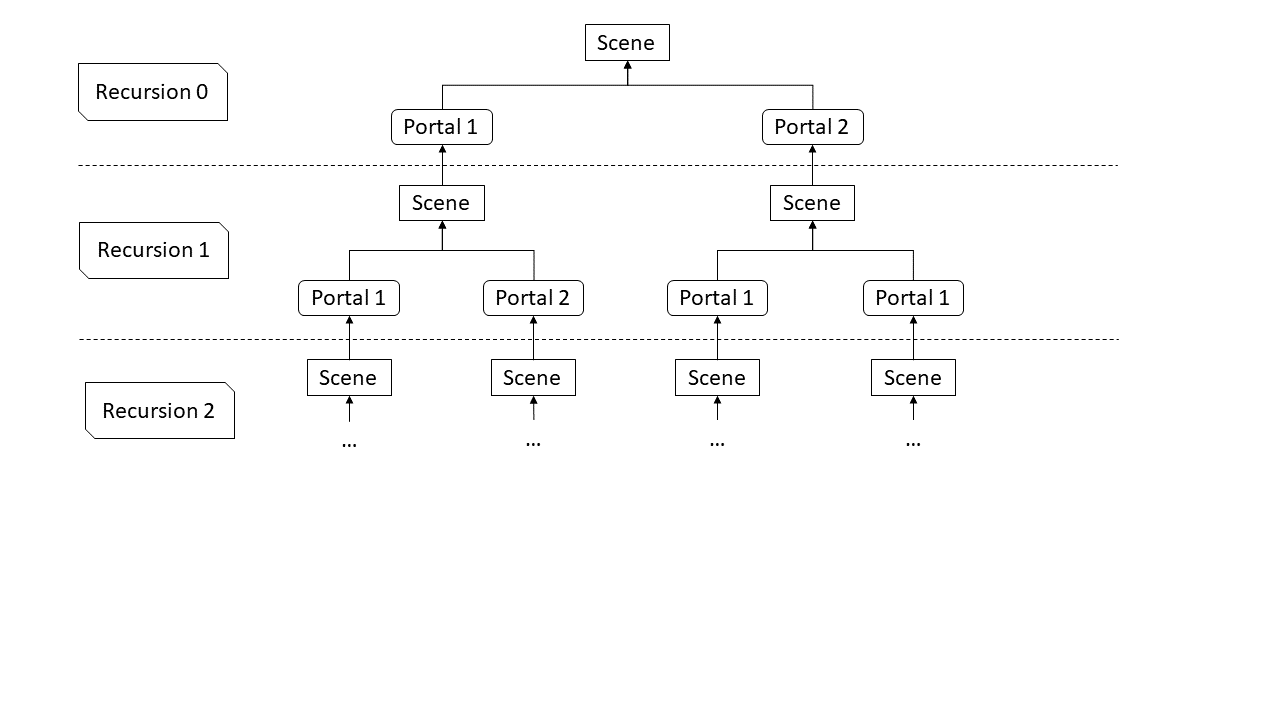
\includegraphics[width=\linewidth]{images/rendertree.png}
	\caption{Render Dependencies}
	\label{fig:rendertree}
\end{figure}


When drawing multiple portals recursively, the draw dependencies can be imagined as a tree. Figure~\ref{fig:rendertree} shows the dependencies for two portals. In \textit{recursion 0} the two portals can only be drawn after the all objects were drawn. Otherwise portals that are occluded by an object might wrongly mark the pixel in the stencil buffer. Both draws of all objects in \textit{recursion 1} can only be drawn when their respective portal was already drawn. However, it is not necessary that all portals from \textit{recursion 0} were drawn, before objects can be drawn in \textit{recursion 1}. For example, in \textit{recursion 0} portal 1 could be drawn first. Then the objects from \textit{recursion 1} that depend on that portal can be drawn. After this portal 2 from \textit{recursion 0} can be drawn.

There are two approaches on the drawing order: depth-first or breadth-first. With depth-first order, the contents of portal 1 in \textit{recursion 0} would be fully complete, before it begins drawing the contents of portal 2 in recursion 0. Depth-first order only requires a small number of different values to mark pixels. When going down the tree, a different value can be used for each recursion. When going up, that value is not needed anymore and can be recycled. However, an implementation must make sure that no unneeded value remains in the stencil buffer. A downside is, that the draws are fully dependent on each other.

Breath first draws one recursion completely before drawing the next recursion. The number of different values needed to mark a pixel, scales super-linearly with the \gls{portalcount} and \gls{recursioncount}. One value is needed for each portal in a recursion. For a scene with two portals, at least needs 4 different values besides 0 are needed to mark all portals from \textit{recursion 1}. For \textit{recursion 2} 8 values are needed. As the stencil buffer usually being limited to 8 bits this can be quickly become a hard limit. However, the advantage is that the depth buffer needs to be cleared less often, only when transitioning between recursions. Additionally, within a recursion there are no dependencies between the multiple draws of objects, as well as the portal draws.

Previous transformative portal implementations used depth-first \cite{lowe:2005:technique,lecture:portalProblems}. The implementation presented in this thesis uses breadth-first. There are fewer dependencies between the draws, which can be exploited. Additionally, similar draws can be grouped, which reduces the number of render passes. Both the number of draw call as well as the number of stencil values needed scale super-linearly. The author believes it is more likely that the number of draws will be the limiting factor, rather than running out of values in the stencil buffer.



\subsection{Generating View Matrices}
\label{section:generatingviewmatrices}


As describe in section~\ref{section:textursVsStencil}, the scene needs to be rendered from the correct viewpoint. When looking through the portal, it must look as if the camera looks directly at the object.

\begin{figure}[H]
	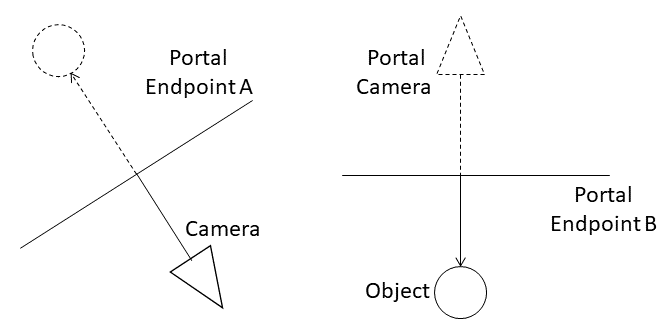
\includegraphics[width=\linewidth]{images/portal.png}
	\caption{A \gls{portalpair} connecting two parts of the world}
	\label{fig:portal}
\end{figure}

Figure~\ref{fig:portal} shows the camera looking at endpoint A of a portal pair. It appears as if the dotted circle is in front of the camera. However, the actual circle is somewhere else. Instead of seeing endpoint A, the contents of the other part of the world are seen from the portal camera's viewpoint.


To move the camera to the correct location, the \gls{endpoint}['s] \gls{teleportationmatrix} is applied to the \gls{cameramatrix} to calculate the portal camera. Then the portal's \gls{viewmatrix} can be obtained by inverting the portal camera.

%This viewpoint corresponds to the camera's viewpoint teleported by the specific portal's \gls{teleportationmatrix}. As the camera moves the matrices must be calculated every frame.

%\begin{figure}[H]
%	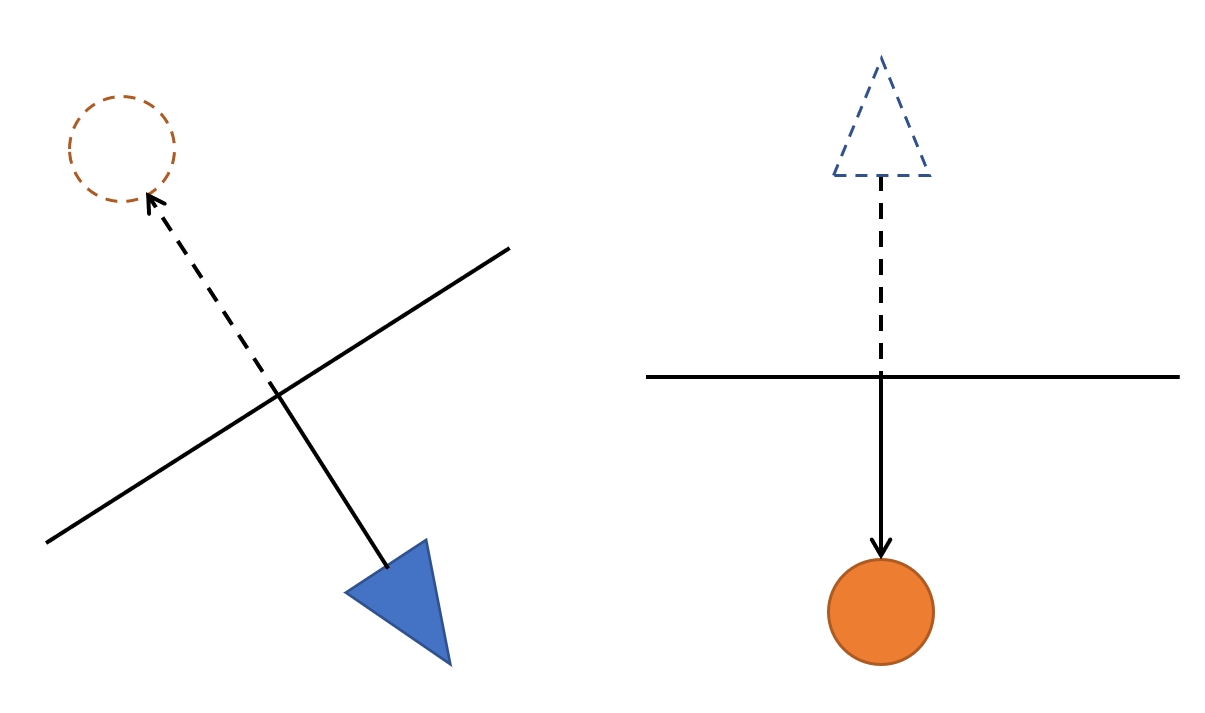
\includegraphics[width=\linewidth]{images/camera_matrices.png}
%	\caption{Portal Camera}
%	\label{fig:cameramatrices}
%\end{figure}

%Figure~\ref{fig:cameramatrices} shows two portal endpoints. The blue triangle represents the camera and the orange circle represents an objects. The dotted blue triangle represents the portal view camera.



\subsection{Recursive Portal Matrices}
\label{section:recursivecameramatrices}
The previous section explained how to calculate the camera matrices for each portal for \textit{recursion 1}. For \textit{recursion 2} the camera's viewpoint must be transformed twice by two sequential applied \glspl{teleportationmatrix}. This needs to be done for every permutation of two portals. For \textit{recursion 3} this is done for every permutation of three portals and so forth. These different permutations of matrices form a tree. The root is the current \gls{cameramatrix}. The matrix of child node n is equal to its parent matrix multiplied by portal n's \gls{teleportationmatrix}. The tree is filled level by level, each level reusing the calculations of the previous level.




The tree of camera matrices is stored in an array. The indices can be found the following way:

\begin{itemize}
	\item $ n^{th} child = current index * portalcount + 1 + n$
	\item $ parent = \lfloor(current index-1)/portal count\rfloor $
\end{itemize}



%%$c_n .. nth child index$
%%$p .. parent index$
%%$i ... curent index$
%%$t ... portal count$

\begin{figure}[h]
	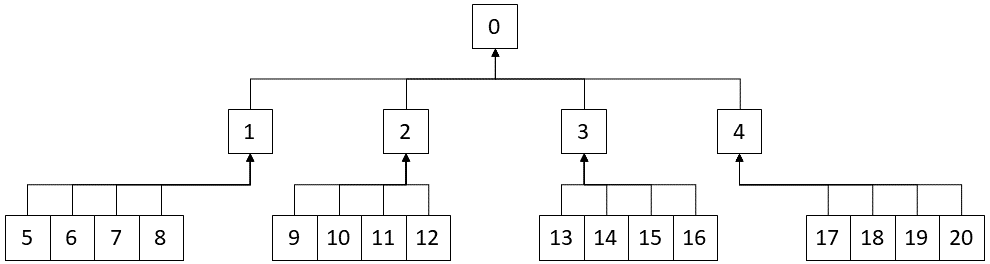
\includegraphics[width=\linewidth]{images/cameraindices.png}
	\caption{Camera Indices}
	\label{fig:cameraindices}
\end{figure}

Figure~\ref{fig:cameraindices} shows the indices for four portals, with two iterations. For example, to find the view matrix of portal 0, seen through portal 1, we would access the array at index 9. Note that the size of the tree scales exponentially, with the \gls{recursioncount}, as all possible permutations of portals need to be covered. When the calculation of the tree is finished, every matrix in the tree is inverted.


\subsection{Dual Depth Buffer}

When drawing the scene from the portal's view, care must be taken to not draw objects that are between the camera and other endpoint. In previous works this is often referred to as clipping \cite{lowe:2005:technique}.
\begin{figure}[h]
	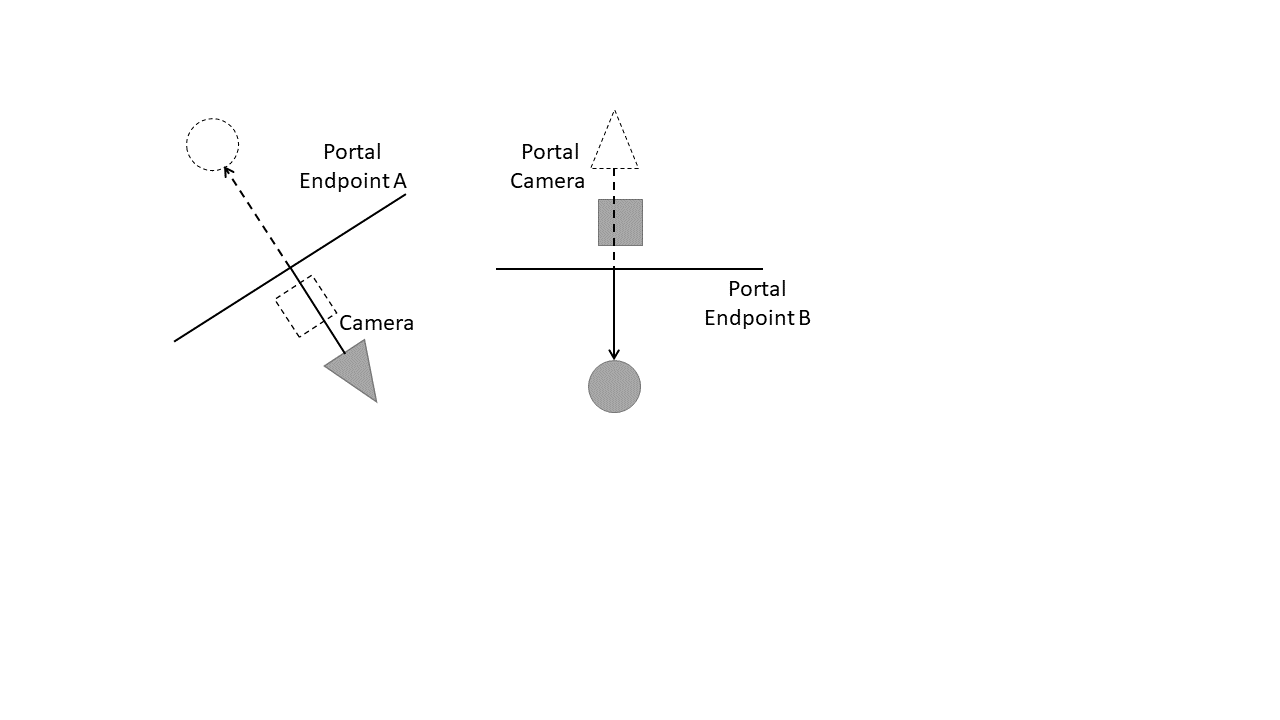
\includegraphics[width=\linewidth]{images/bananajuce.png}
	\caption{Object between portal camera and portal endpoint}
	\label{fig:bananajuce}
\end{figure}

Figure~\ref{fig:bananajuce} shows such an example. Without additional techniques the square would be drawn. One possibility would be the use of clip planes. However, this limits a portal's shape to planes. Another solution, which allows for arbitrary portal shapes, is to use two depth buffers or dual depth buffer: a \gls{neardepthbuffer} and a \gls{fardepthbuffer}. The \gls{fardepthbuffer} is used to discard fragments with a greater depth value. The \gls{neardepthbuffer} discards fragments with a lesser depth value. When rendering a portal, its depth is also rendered to the near buffer. The box's depth values from figure~\ref{fig:bananajuce} are closer than the \gls{neardepthbuffer} values and the box's fragments are discarded \cite{lowe:2005:technique, ropinski:2004:real}.

In this implementation the hardware supported depth buffer is used as the \gls{fardepthbuffer}. For the \gls{neardepthbuffer} two buffers in form of colour textures are used, a \gls{readnearbuffer} and a \gls{writenearbuffer}. This way an old \gls{neardepthbuffer}'s values can be used, while writing new \gls{neardepthbuffer} values. In the fragment shader, the fragment's depth value is compared to the \gls{readnearbuffer}. If it is smaller it is manually discarded, with a discard statement in the shader. Whenever the portals are drawn, they do not only write the \gls{fardepthbuffer} via depth test, but also write to the \gls{writenearbuffer} via colour output. When the prototype transitions to the next recursion, the \gls{writenearbuffer} and \gls{readnearbuffer} are swapped.

Dual buffering the near buffer avoids problems with an edge case: Portal A could occlude portal B and portal B is drawn first. With only one near buffer, portal B would set the near buffer to its depth values. The fragments of portal A would be discarded, instead of occluding portal B.

The \gls{readnearbuffer} is an input attachment and the \gls{writenearbuffer} is a colour attachment. In recursion 0, no \gls{readnearbuffer} test is used.

\subsection{Portal near Z fighting}
\label{section:portalzfighting}
When rendering the contents of one endpoint of a portal pair, the other endpoint would be rendered directly at the same location. They would have the exact same depth value. The other endpoint's fragments would sometimes be discarded by the near buffer and sometimes not. This leads to a special case of Z fighting. To avoid this the winding order of a fragment is stored in the near buffer. When the fragment's depth value and the \gls{readnearbuffer} value are nearly equal and winding order is the same, the fragment is discarded. This is done by increasing the comparison value by some small amount or percentage when winding orders are the same.

For the prototype the depth values range from 0 to 1 and does not use negative values. This property enables storing the winding order as the sign of the near buffer. Positive depth values indicate front facing primitives and negative depth values indicate back facing primitives. Near depth comparison is done with the absolute value of the buffer.

\subsection{Stencil Values and compare masks}
\label{section:stencilcomparemasks}

As the prototype uses the breadth-first approach, it cannot use the stencil increment and decrement technique described in other works \cite{schmalstieg:1999:sewing, lowe:2003:fragment, lecture:portalProblems}. Directly setting the stencil value can be achieved by setting a reference value and using the replace stencil operation. However, the stencil reference is also used for the comparison. This means that the same value for is used comparison as well as writing. This can be achieved with the stencil compare mask and by prepending stencil values.

\begin{figure}[h]
	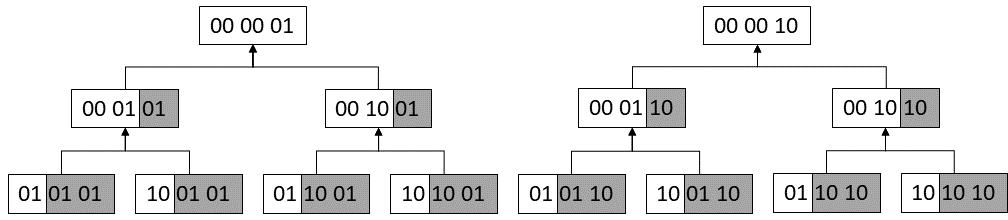
\includegraphics[width=\linewidth]{images/stencilvalues2.png}
	\caption{Compare Mask and Stencil Values}
	\label{fig:stencilvalues}
\end{figure}

Figure~\ref{fig:stencilvalues} shows this process with two portals and 6 bits. The grey part is used for comparisons, while the whole value is used to write. The comparison mask of \textit{recursion 0} masks out all bits. For \textit{recursion 0}, the stencil test is always successful. For two portals, \textit{recursion 1} masks out all but the last two bits. Notice that the last two bits of \textit{recursion 1}'s stencil values are the same as their respective parent values. It is important that the stencil values start with 1 and not with 0, otherwise they would not distinguishable from their parent values.

This also means that the range of values is one less than representable by the number of bits. This is very significant, as the portals come in pairs. Scenes with two and four portals each require one more bit than normally needed. Since the stencil buffer usually only has eight bits, this limits the number of recursions considerably.



\section{Initial Implementation}
\label{section:intialimplementation}
This section describes the first iteration of the prototype. It uses the specified techniques described in section~\ref{section:portaldrawing} and focuses on how those are implemented.


\subsection{Render Pass Setup}
\label{section:renderpasssetup}

The implementation uses just one render pass with multiple subpasses. This allows for the use of input attachments and potentially enables the \gls{gpu} driver to optimize. For example, many images are only needed within the render pass and do not need to be transferred anywhere else.

\begin{figure}[h]
	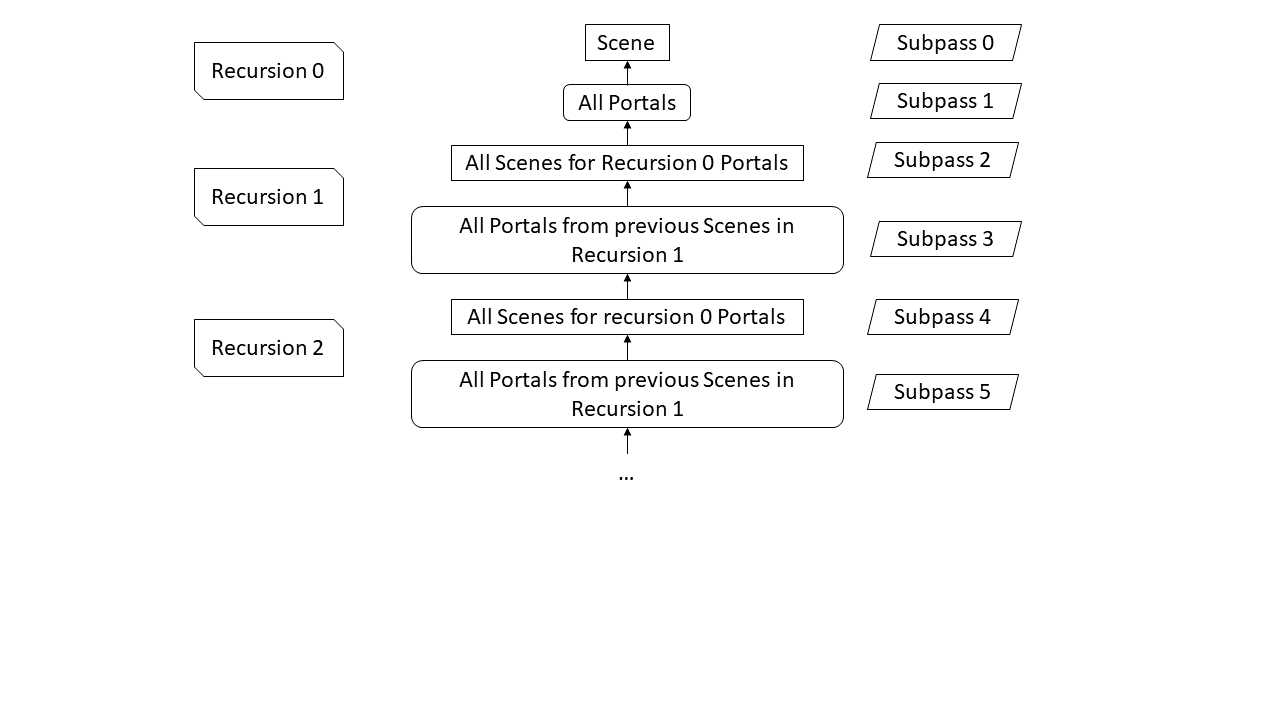
\includegraphics[width=\linewidth]{images/renderpasses.png}
	\caption{Subpasses and work done}
	\label{fig:renderpasses}
\end{figure}


Figure~\ref{fig:renderpasses} shows the subpasses, which recursion they belong to and what work is done. Notice that compared to figure~\ref{fig:rendertree} all object and portal draws are batched together. Every even subpass is responsible for drawing objects, while in every odd subpass the portals are drawn. The subpass index divided by two equals the recursion index. 

\begin{figure}[h]
	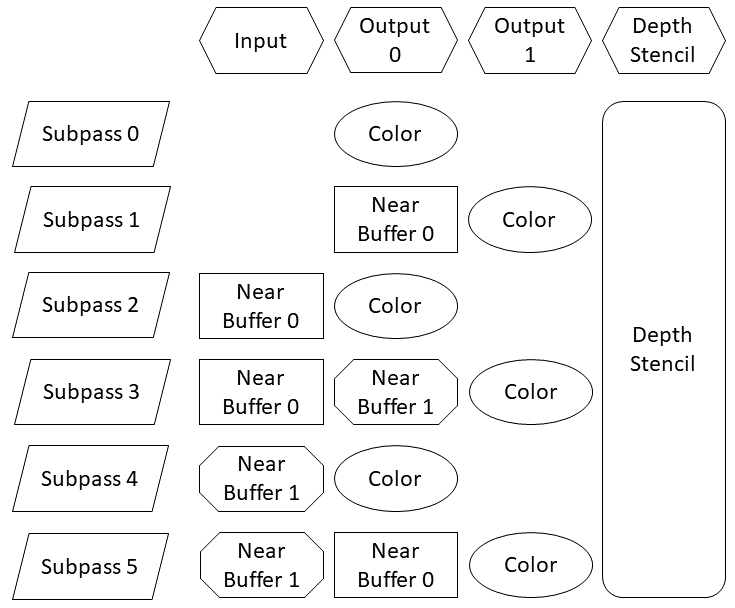
\includegraphics[width=\linewidth]{images/attachmentsetup.png}
	\caption{Attachment Setup}
	\label{fig:attachments}
\end{figure}

Figure~\ref{fig:attachments} illustrates the attachments of the individual subpasses for two recursions. Odd subpasses write into the near buffer, which is used as input for the following two subpasses.  Note that output 1 is not really necessary as portals do not need to write colour. However, for this implementation it was kept for debugging purposes. The last subpass does not need to write to the near buffer, as there are not later subpasses which could use it. It is kept for debugging purposes too. The depth stencil attachment is never changed. The colour and depthstencil attachments are cleared at the beginning of the render pass with VK\_ATTACHMENT\_LOAD\_OP\_CLEAR. Both near buffers use VK\_ATTACHMENT\_LOAD\_OP\_DONT\_CARE. The stencil test ensures that they are only accessed at locations where portals have previously written a value. Each subpass has set a dependency in the fragment shader on the previous subpass' output. The depth part of the depth stencil buffer is cleared after each recursion.


\subsection{Graphic Pipelines}
When rendering multiple scenes one after each other, as well as when rendering a different portal, the stencil reference needs to be changed. There are two ways to solve this problem: either using multiple pipelines or using dynamic pipeline state. For the prototype dynamic pipeline state was used, as the number of graphic pipelines needed would scale super-linearly with the number of portals and recursions. Dynamic state seemed much easier to manage in comparison.

However, the subpass index cannot be dynamic state. Thus, even with dynamic stencil references, there must be at least the same number of graphic pipelines as there are subpasses. If more than one shader is used for rendering scene objects or portals, additional graphic pipelines are needed. Each additional shader increases the number of graphic pipelines by half of the number of subpass, as it is either only used for portal rendering or only for scene rendering. Since there already are different pipelines for the subpasses, each of them can have a different stencil compare mask (see section~\ref{section:stencilcomparemasks}). There is no need for dynamic stencil compare masks.

Graphic pipelines for both scene and portal drawing, have face culling disabled. Portals do not have to be watertight and scene objects might be transformed in a way that changes their winding order. If it is ensured that there are no teleportation matrices that could change the winding order, face culling can be enabled for scene objects. For this implementation it was chosen to support these kinds of teleportation matrices.

The individual graphic pipelines for drawing the scene differ by subpass index and stencil compare mask. This is also true for the graphic pipelines used for portal drawing. Additionally, \textit{subpass 0} has the stencil test completely disabled, while \textit{subpass 1} uses an always succeeding test with VK\_STENCIL\_OP\_REPLACE. Other even subpasses use the stencil compare op VK\_COMPARE\_OP\_EQUAL with VK\_STENCIL\_OP\_KEEP for all depthstencil test results. Odd subpasses use VK\_COMPARE\_OP\_EQUAL with VK\_STENCIL\_OP\_REPLACE when both tests succeed and  VK\_STENCIL\_OP\_KEEP otherwise.

\subsection{Shaders}
Vulkan requires the SPIR-V format. The shaders are written using \gls{glsl} and are compiled using the \gls{glsl} Validator (glslangValidator.exe) from LunarG's Vulkan SDK. All fragment shaders contain a manual check with the near buffer. If it fails, the fragment is discarded using the discard statement. However, for \textit{subpass 0} and \textit{subpass 1} there is no input attachment (see figure~\ref{fig:attachments}). For those shaders the check is omitted. To prevent shader redundancies, the shader is compiled twice. One of the compilations skips the check using the preprocessor of the \gls{glsl} Validator. As previously mentioned in section~\ref{section:renderpasssetup}, the portals drawn in the last subpass do not need to store anything in the near buffer. This could also be omitted using conditional compilation. All scene objects only have one colour. It is passed via push constants. Additional minimal shading is performed using diffuse-only shading with a fixed directional light.

Vertex shaders need to transform the vertices for every possible view position. The different view matrices are stored in a \gls{ubo}. The index to access the current view matrix is received via push constant. The model matrix is received also via push constant, since it changes per model and it there was still enough space in the push constant. The perspective matrix is passed via \gls{ubo}, as it never changes. Even if it would change this would be at most once per frame. The vertex shaders for all objects and portals respectively. No conditional compilation is needed.


The shaders are automatically recompiled after a change, using Visual Studio's Custom Build Tool feature. This enables fast iteration times and avoids errors due to forgetting to compile.

\subsection{Pre draw steps}

In this implementations, old command buffers are reused, by resetting their command pool. However, it could be possible that these commands are still being executed. Furthermore, buffers might also be in use and writing them could be dangerous. First, a fence is used to wait until it is safe to reuse the resources.

Then, the camera matrices and perspective matrix are calculated. Both \glspl{ubo} use host visible memory, so the result is written to them via memory mapping. Since their memory is also host coherent, no explicit flushes are needed.
Next, the index for next image to be rendered is acquired. A semaphore is passed, which can be waited on before submitting the command buffer until the image is available. Otherwise, it could be possible to write to the image, that is currently displayed on the screen.
Finally, the command pool reset and the corresponding command buffer is ready for recording.

\subsection{Recording the Command Buffer}

In this section all functions calls are member functions of the command buffer, as the Vulkan C++ \gls{api} is used. These commands are formatted in \textbf{bold}. In the Vulkan C \gls{api} these commands are not member function. Instead they are free functions with their name prefixed by \textit{vkCmd} and taking the command buffer as their first parameter.

First, \textbf{begin} called with a parameter to indicate that the command buffer is used for a one-time submit. Then the render pass is begun with \textbf{beginRenderPass}.

%Instanced drawing is not used so instance count is 1 and first instance is 0 for \textbf{drawIndexed} calls.

Subpass 0 does not use the stencil buffer, so no reference needs to be set. Before drawing the objects \textbf{bindIndexBuffer} and \textbf{bindVertexBuffer} are called. All object vertices reside in the same buffer, so this only needs to be done once. Then for every object \textbf{pushConstants} is called to set the push constants for that object, followed by \textbf{drawIndexed} to draw the object. 

First, to change to \textit{subpass 1}, \textbf{nextSubpass} is called. Next, similar to \textit{subpass 0}, \textbf{bindIndexBuffer} and \textbf{bindVertexBuffer} is called. After that, for each portal the corresponding stencil value (see section~\ref{section:stencilcomparemasks}) is set dynamically with \textbf{setStencilReference}. Finally, \textbf{pushConstants} is called followed by \textbf{drawIndexed}.

Subsequent even subpasses are similar to \textit{subpass 0}, but all objects are drawn multiple times. At the begin of drawing all objects one time, \textbf{setStencilReference} is called with corresponding stencil value used in the previous subpass. Each scene is drawn with a different \gls{cameramatrix} id, which is specified via push constant. 

Subsequent odd subpasses are similar to \textit{subpass 1}, but all portals are drawn multiple times. Each portal uses a different stencil reference.  At the begin of drawing all portals one time, the stencil compare mask is set dynamically with \textbf{setStencilCompareMask}. Similar to the objects, each draw of all portals uses different \gls{cameramatrix} id specified via push constant. 

In total all objects and all portals are drawn for each possible permutation of portals. The number of draws for each of them is equal to the size of the view matrix array.


\section{Dynamic Portal Rendering}
One downside of the initial portal rendering strategy was its hard limit of total portals in the scene. It did not matter whether a portal was visible or not, it was always drawn and used up values in the stencil buffer. For two recursions, only 15 or less portals were allowed to exist in the scene. For three recursions only 7 or less, and for four recursions only 3 portals were possible. For this reason, a new method was derived which is limited by the visible portal count instead of the total portal count. 

When drawing a portal, it uses a stencil value depending on the number of visible portals drawn before it, instead of using a fixed value. However, this also means that the right camera index cannot be known before submitting.


\subsection{View Matrix Selection}
\label{section:viewmatrixselection}
Except for \textit{subpass 0} and \textit{subpass 1}, it is not possible to know which camera index to access, since this depends on what portals were drawn previously. This problem is solved with an indirection.

\begin{figure}[h]
	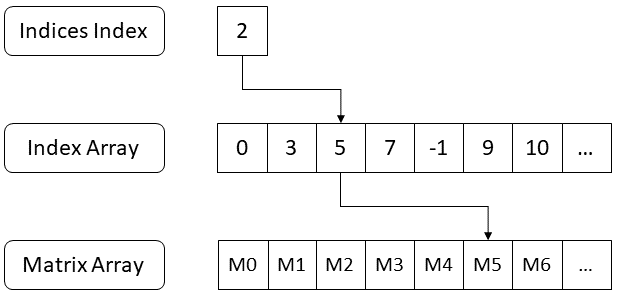
\includegraphics[width=\linewidth]{images/viewmatrixindirection.png}
	\caption{View Matrix Indirection}
	\label{fig:viewmatrixindirection}
\end{figure}

Figure~\ref{fig:viewmatrixindirection} shows an example how this works. Instead of receiving the index for the view matrix, an \textit{indices index} is received. The \textit{indices index} is used to access an element in an \gls{indexarray}. This element's value is the actual index, which is then used to find the correct view matrix in the \textit{matrix array}.

Sometimes there are less visible portals than the maximum count. This cannot be known before submitting the command buffer. The draw commands for elements with invalid portals are still recorded in the command buffer. This implementation uses a special value -1 in the \gls{indexarray} to indicate such a case. It is an invalid index. The value of the view matrix index is the same for every vertex shader invocation of a mesh, as it depends on a push constant value. When encountering an invalid index as view matrix index, the vertex shader sets \textit{gl\_Position} to a fixed position. All vertices of an object will have the same position. All its triangles become degenerate and are culled \cite{khronos:vulkan:spec1.1}.

\begin{lstlisting}[caption={View Matrix Selection}, label=listing:viewmatrixselection]
// shader.vert
#version 450

...

layout(push_constant) uniform PushConstant {	
	mat4 model;
	int viewMatrixIndicesIndex
	...
} pc;

layout(set = 1, binding = 0) uniform GlobalRenderData {
	mat4 proj;
} u_grd;

layout(set = 2, binding = 0) uniform CameraMats
{
	mat4 mats[maxCameraMatCount];
} u_cMats;

layout(set = 4, binding = 0) buffer ViewMatIndices {
	int vIndices[];
} vi;

layout(location = 0) in vec3 inPosition;

const int invalidmatIndex = -1;

void main()
{
	int viewMatIndex = pc.viewMatrixIndicesIndex == 0 ? 
		0 : vi.vIndices[pc.viewMatrixIndicesIndex];
	
	if(viewMatIndex != invalidmatIndex)
	{
		gl_Position = u_grd.proj * u_cMats.mats[viewMatIndex]
		 * pc.model * vec4(inPosition, 1.0);
	}
	else
	{
		// invalid index, create degenerate triangles
		// by setting every vertex to the same value
		gl_Position = vec4(1);
	}
	...
}

\end{lstlisting}

Listing~\ref{listing:viewmatrixselection} shows the code of the vertex shader. Note that if the indices index is 0, it must be recursion 0. 0 can then be used as index for the camera matrices. This is convenient when filling the index buffer later.

\subsection{Properties of the Index Array}
\label{section:indexarrayproperties}

In the prototype the maximum visible portal count can differ for each recursion. This is useful, as in \textit{recursion 0} the draw fills the whole screen, resulting in more visible portals. The contents within portals cover much less screen-space, so it is less likely that portals can be seen within them. For each recursion the screen-space which is drawn will get even smaller. This means \textit{recursion 0} will likely need the most visible portals, while the future recursions will need less and less visible portals.

\begin{figure}[h]
	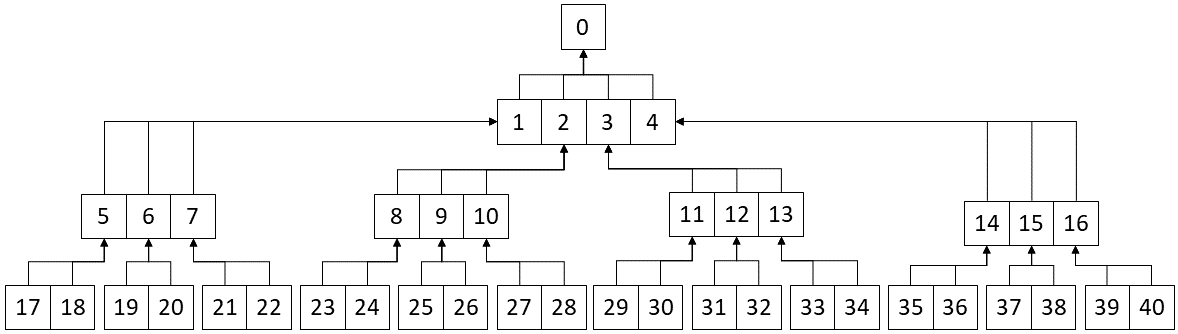
\includegraphics[width=\linewidth]{images/indexarray.png}
	\caption{Index array as tree for 4-3-2 visible portals}
	\label{fig:indexarray}
\end{figure}

The indices array is a tree within an array, similar to the view matrix array. However, due to the different number of visible portals for each recursion, the number of children differs for each tree level. Figure~\ref{fig:indexarray} illustrates the connections between the elements. The shown tree supports three recursions. The visible portal count for the first recursion is four, for the second one it is three and the third recursion one it is two. The tree has one root. Each element's child count corresponds to its level in the tree.

The following terms are used for index calculation formulas:
\begin{itemize}
	\item $L_n$ ... the n\textsuperscript{th} level,
	\item $LC_n$ ... the element count of the n\textsuperscript{th} level
	\item $LF_n$ ... the index of the first element of the n\textsuperscript{th} level
	\item $LDC_n$ ... the number of direct child nodes for each element in the n\textsuperscript{th} level. 
	\item $L_nE_i$ ... the index of the i\textsuperscript{th} element in the n\textsuperscript{th} level
	\item $L_nE_iC_k$ ... the index of the k\textsuperscript{th} child of the i\textsuperscript{th} element in the n\textsuperscript{th} level 
\end{itemize}

The following formulas can be used to calculate indices:

\begin{itemize}
	\item $LC_0 = 1$
	\item $LC_n = LC_{n-1} * LDC_{n-1}$
	\item $LF_0 = 0$
	\item $LF_n = LC_{n-1} + LF_{n-1}$
	\item $L_nE_iC_k = LF_{n+1} + LDC_{n} * i + k$
\end{itemize}

For every recursion the whole corresponding level of the \gls{indexarray} tree is traversed, drawing each object and portal a total of $LC_n$ times. Using figure~\ref{fig:indexarray} as example, every object and portal in \textit{recursion 0} is drawn once. For \textit{recursion 1} and \textit{recursion 2} they are drawn 4 and 12 times respectively. Finally, for the last recursion, recursion 3, everything is drawn 24 times. In total 41 draws would be issued for each object and portal.

\subsection{Filling the Index Array}
For a correct indirection the \gls{indexarray} must be filled with correct values. Before starting to record draw commands, the \gls{indexarray} is filled with an invalid index value by calling \textbf{fillBuffer} on the command buffer, in the pre draw step. Listing~\ref{listing:indicesindexcalculation} shows the algorithm used by the fragment shader to calculate and set the individual \gls{indexarray} elements.

\begin{lstlisting}[caption={Calculating Indices Index}, label=listing:indicesindexcalculation]
// shader.vert
#version 450
...
layout(push_constant) uniform PushConstant {	
	int viewMatrixIndicesIndex;
	int maxVisiblePortalCount;
	int portalIndex;
	int maxPortalCount;
	int nextLevelStartIndex;
	int portalGroupIndex;
	...

} pc;

layout(set = 4, binding = 0) buffer ViewMatIndices {
	int vIndices[];
} vi;

void main()
{
	...
	int previousVisiblePortalCount = ...
	
	if(previousVisiblePortalCount < pc.maxVisiblePortalCount)
	{
		int currentViewMatIndex = pc.viewMatrixIndicesIndex == 0 ? 
			0 : vi.vIndices[pc.viewMatrixIndicesIndex];
		
		int firstPortalViewIndex = 1 +
			(currentViewMatIndex * pc.maxPortalCount);
		
		int currentPortalViewIndex = firstPortalViewIndex +
			pc.portalIndex;
		
		int firstViewIndicesIndex = pc.nextLevelStartIndex +
			(pc.portalGroupIndex * pc.maxVisiblePortalCount);
			
		int viewIndicesIndex = firstViewIndicesIndex +
			previousVisiblePortalCount;
			
		atomicCompSwap(vi.vIndices[viewIndicesIndex], -1, currentPortalViewIndex);
	}
	...	
}

\end{lstlisting}

For each portal's fragment shader, the previous visible portal count is calculated, which is explained in the next section. It is then compared with the maximum visible portal count. If it the previous visible portal count is higher or equal to the maximum visible portal count, the \gls{indexarray} is not written by the shader.

Otherwise the index for writing is calculated using $L_nE_iC_k = LF_{n+1} + LDC_{n} * i + k$ (see section~\ref{section:indexarrayproperties}). $LF_{n+1}$ is provided by via push constant and stays the same for the whole recursion. $LDC_{n}$ is also the maximum visible portal count, which was used for the previous check. It is provided via push constant and also stays the same for the whole recursion. $i$ is equal to the number of previous \glspl{portalset} for that recursion. This value will be referred to as the \gls{portalsetid} which is unique for each draw of a \gls{portalset} in within a recursion. It is provided via push constant. $k$ is equal to the number of previous visible portals.

Using the formula $ n\textsuperscript{th} child = current index * portalcount + 1 + portalId$ from section~\ref{section:recursivecameramatrices} the view index can be calculated. $currentindex$ was the index used in the vertex shader to access the right view matrix. To pass $portalcount$ push constants are used. $n$ is equal to a portal's \gls{portalid} and passed via push constants. Now the view index is written to the right location in the \gls{indexarray}.

Every fragment shader invocation will either write the same value or write nothing at all. If nothing was written to an \gls{indexarray} element, it will have its initial invalid index value. For the last portal iteration a visible portal count of 0 is passed. This is an indicator that it is the last recursion. This prevents the portals from writing past the end of the \gls{indexarray}.

\subsection{Previous Visible Portal Count Algorithm}
\label{section:visibleportalcount}
A portal is visible if at least one fragment of it was drawn. One common way of finding out whether fragments were drawn are occlusion queries. Reading back the result of an occlusion query to the \gls{cpu} was deemed too slow. Although Vulkan also supports copying the result to a buffer by calling \textbf{copyQueryPoolResults} on a command buffer, this is only possible outside of a render pass. For this reason, a different way of finding the visible portal portals was derived.

The algorithm uses a \gls{helperarray} with integer elements and each drawn \gls{portalset} exclusively owns a range within it. No other group may read from or write to that range. The first index of the range is called \gls{firsthelperindex}. The size of the range is equal to the \gls{portalcount}. Each portal in a group has an element within range, where it has exclusive write access. It is called \gls{currenthelperelement}. The index to that element is called \gls{currenthelperindex}. Before starting to draw each element of the \gls{helperarray} is set to 0.

\begin{lstlisting}[caption={Calculate Previous Visible Portals}, label=listing:previousvisibleportals]
// portal.frag
#version 450
#extension GL_ARB_shader_stencil_export : enable

...
layout(push_constant) uniform PushConstant {	
	int maxVisiblePortalCount;
	int portalIndex;
	...
} pc;

layout(set = 5, binding = 0) buffer PortalIndexHelper {
	int indices[];
} pih;

void main()
{
	...
	int previousVisiblePortalCount = 0;
	int currentHelperIndex = pc.firstHelperIndex + pc.portalIndex;
	
	// stop at currentHelperIndex as we are not allowed to read it
	// and the following elements were not written yet
	for(int i = pc.firstHelperIndex; i < currentHelperIndex; ++i)
	{
		previousVisiblePortalCount += (pih.indices[i]) == 0 ? 0 : 1;
	}
	
	if(previousVisiblePortalCount < pc.maxVisiblePortalCount)
	{
		atomicCompSwap(pih.indices[i], 0, previousVisiblePortalCount);
		...
	}
	...
}
\end{lstlisting}

Listing~\ref{listing:previousvisibleportals} shows the fragment shader algorithm. Each portal's fragment shader iterates from the \gls{firsthelperindex} to \gls{currenthelperindex} excluded. These indices are used to access elements of the \gls{helperarray}.  The counter is incremented, each time that element is not zero. This count is equal to the number of previous visible portals and can be used for future calculations. Before drawing the next portal, a pipeline barrier is inserted, so that the writes of current portal's fragment shader are visible to the next portal's fragment shader.

This algorithm makes use of the following property: If the fragment shader is never invoked, it will never write a value to its \gls{currenthelperelement}. If multiple shader invocations write the same non-zero value to the \gls{currenthelperelement} there will be that value, no matter how many shader invocations have written to it.
Thus, if at least one fragment shader was invoked for the portal, there will be a non-zero value at its position. When writing to the element in one shader, other shader invocations are not influenced, as this element is never read from. There is no race condition. The iteration does not need to continue after \gls{currenthelperelement}, as these values will not have been written yet and will remain 0.

The written value may can be any non-zero value, but writing the previous visible portal count allowed for easier debugging during the creation of the prototype.

\subsection{Properties of the Helper array}
\label{section:helperarrayproperties}
The \gls{helperarray} and \gls{indexarray} have a similar structure. For each element in the \gls{indexarray}, a \gls{portalset} is drawn. During the draw of one \gls{portalset}, \gls{portalcount} elements of the \gls{helperarray} are used. For the last recursion no indices need to be calculated, as nothing will be drawn after it. Thus, the element count of the \gls{helperarray} can be calculated by multiplying the element count of the \gls{indexarray}, without its last level, with the \gls{portalcount}.

\begin{figure}[h]
	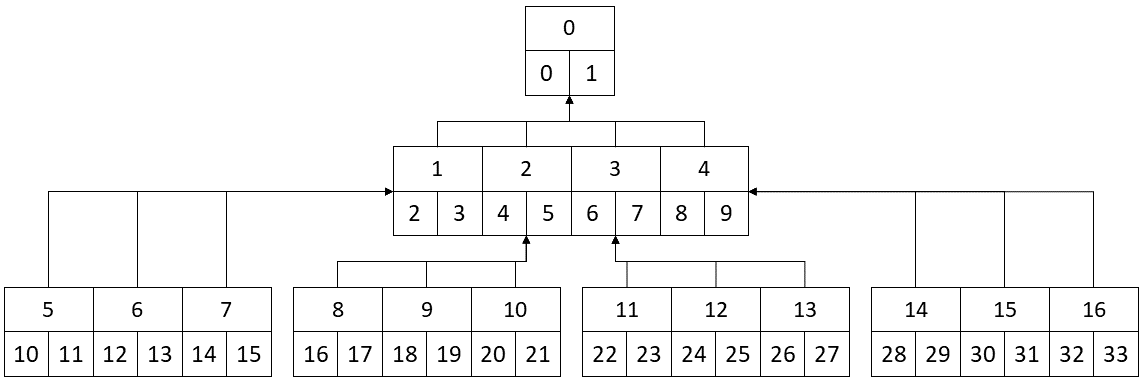
\includegraphics[width=\linewidth]{images/helperarray.png}
	\caption{Helper array as tree for 4-3-2 visible portals, with \gls{portalcount} of 2}
	\label{fig:helperarray}
\end{figure}

Figure~\ref{fig:helperarray} shows the \gls{helperarray} as tree, with a \gls{portalcount} of 2. It uses the same recursion count and visible portal count as the \gls{indexarray} of figure~\ref{fig:indexarray}. The top number in the bigger rectangle corresponds to the index helper tree for easier comparison. Notice that the first index of the elements in the bottom boxes is equal to the top number multiplied by \gls{portalcount}. This first index corresponds to the individual \textit{First Helper Indices}. The same formulas as described in section~\ref{section:indexarrayproperties} can be used to calculate those indices. They first need to be divided by the \gls{portalcount}, then used in the formula and the result multiplied by \gls{portalcount}.


\subsection{Calculating the Stencil Reference}
Before drawing, it is not known how which and how many portals are visible. The stencil reference value cannot be set dynamically while recording the command buffer. Instead the stencil reference is calculated in the shader and set via the Vulkan extension VK\_EXT\_shader\_stencil\_export. Since this is an extension this feature is not supported on every \gls{gpu}.

\begin{lstlisting}[caption={Calculate Stencil Reference in Shader}, label=listing:stencilcalculation]
// portal.frag
#version 450
#extension GL_ARB_shader_stencil_export : enable

// ...
layout(push_constant) uniform PushConstant {	
	uint parentStencilReference;
	int stencilReferenceBits;
	int maxVisiblePortalCount;
//...
} pc;

out int gl_FragStencilRefARB;

void main()
{
	...
	int previousVisiblePortalCount = ...
	
	if(previousVisiblePortalCount >= pc.maxVisiblePortalCount)
	{
		...
		uint myStencilReference = previousVisiblePortalCount + 1;
		uint stencilReference = pc.parentStencilReference 
		| myStencilReference << pc.stencilReferenceBits;
		gl_FragStencilRefARB = int(stencilReference);
	}	
	...
}
\end{lstlisting}

Listing~\ref{listing:stencilcalculation} illustrates the calculation. The current stencil reference is passed via push constants. This value changes per drawn \gls{portalset}. It corresponds to the stencil reference used by the visible portals of the previous recursion. The fragment shader calculates the number of previous visible portal and adds 1 to calculate the stencil prefix. Using 0 as stencil prefix would lead to ambiguities (see section~\ref{section:stencilcomparemasks}). That stencil prefix needs to be shifted by the number of bits used by parent stencil reference and then bitwise ORed together. Shifting is done using unsigned types to avoid potential undefined behaviour.

\subsection{Atomic Writes to Storage Buffer Objects}
In listing~\ref{listing:indicesindexcalculation} and~\ref{listing:previousvisibleportals} \textit{atomicCompSwap} was used to write to the storage buffer objects. This avoids potential problems due to race conditions. However, it needs to be investigated if these are really needed. The written values are never read during the shader invocations of one portal. Before they are read by another portal, there is always a memory and execution barrier. For the prototype the atomic operations were left in, as they did not affect performance.

\section{Dynamic Portal instance rendering}
\label{section:dynamicportalinstancerendering}
Dynamic portal rendering shifted the limit from maximum portals in a scene to maximum visible portals, while also improving performance. However, the prototype still had possibilities for improvement. All objects and portals were drawn several times for all the visible portals and recursions. Additionally, using stencil export significantly reduces the number of devices the prototype can run on. Since the depth and stencil tests are performed after the fragment shader, portal fragments that would have been discarded by stencil and depth test still counted as visible. This led to two changes in the prototype.

Initially manual stencil testing was tried out. After seeing no notable decrease in performance, the manual test replaced the old stencil test.

Another change was made to batch draws together with instanced rendering. Most changes to the code were loop transformations. Listing~\ref{listing:looptransform} shows the difference in pseudo code.

\begin{lstlisting}[caption={Pseudocode Loop Transformation}, label=listing:looptransform]
// old 
for(int i = 0; i < previousPortalCount; ++i)
{
	commandBuffer.setStencilRefrence(stencilReferences[i]);
	for(int k = 0; k < sceneObjectCount; ++k)
	{
		commandBuffer.pushConstants();
		commandBuffer.drawIndexed(sceneObjects[k], 1);
	}
}

// new
for(int i = 0; i < sceneObjectCount; ++i)
{
	commandBuffer.pushConstants();
	commandBuffer.drawIndexed(sceneObjects[i], previousPortalCount);
}
\end{lstlisting}


Calculating the stencil references can be simplified. Using the same stencil reference to compare and set the stencil buffer is no longer needed. The stencil reference value now increments by one for each instance. In fact, the stencil reference value and indices index are the same. The indices index for the first instance is passed via push constants. The shaders can calculate their current \textit{indices index} and stencil reference by adding gl\_InstanceIndex to it.

As push constants cannot change between drawing  instances of an object, all uses of the \gls{portalsetid} were replaced with gl\_InstanceIndex.

As the \gls{portalsetid} determines the \gls{firsthelperindex}, all instances of the drawn portal will use a different range in the \gls{helperarray}. They do not interfere with each other. Since there is no synchronisation needed between the instances they can all use instance drawing and have their draw loop transformed similar to the draw loop of objects. However, pipeline barriers are still needed between drawing different portals.

Changing the code to use instance drawing, resulted in a huge performance improvement. Compared to the previous version, the code was six times faster on a particular configuration. Additionally, the manual stencil test allows earlier fragment shader discards, reducing the number of false visible portals. Furthermore, the stencil export extension is no longer required, allowing the application to run on a wider range of graphic cards. Finally, the texture used for the manual stencil test allows for higher stencil values compared to a regular stencil buffer, which is limited to 8 bits. The maximum visible portal count and recursion count is no longer limited by the amount of available stencil values. Those are now only limited by computation speed.


\section{Portal Collision}
One important aspect of portals is moving objects. For this implementation teleporting. was implemented only for the camera, as a proof of concept.

\subsection{Collision Detection}
The camera is imagined as an object without volume. Each time the camera is moved a ray cast is performed from the camera's old location to its new location. The ray intersection is first performed against the portals' \glspl{aabb}. For this test, the method described by \textcite{williams:2005:efficient} was used. If that test passed, the ray is then tested against the portals mesh's triangles. The ray triangle intersection of \textcite{moller:2005:fast} was used to test for triangle intersections.


The triangles and \gls{aabb} are stored in the model space coordinates. This way only one triangle mesh and \gls{aabb} need to be stored for each model that can represent a portal. Before a ray is tested against the \gls{aabb} and triangle mesh, it needs to be transformed into model space. This is achieved by multiplying the portal's inverse model matrix with the origin and direction of the ray.

\subsection{Collision Response}

After a collision with a portal the camera needs to be moved to the correct location. The process is the same as the one used to calculate the viewpoint (see section~\ref{section:recursivecameramatrices}). However, this matrix cannot be directly applied. The camera's position and rotation are not stored as a matrix. An additional matrix was added to the camera object, called \gls{additionaltransform}.

Whenever the camera's position, rotation or \gls{cameramatrix} is needed, they are first modified by the \gls{additionaltransform}. \gls{additionaltransform} is initially equal to the identity matrix. Whenever portal collision occurs, the \gls{additionaltransform} is multiplied with portal's teleportation matrix.



\section{Camera Object Rendering}
When looking through a portal the camera should see itself, being represented by a camera model. However, if that model was rendered in \textit{recursion 0} the view would be inside that model. The implementation avoids this problem, by only conditionally drawing the camera model. In the first subpass drawing the camera is skipped. It is only drawn for subsequent passes.




\chapter{Analysis}
While section~\ref{section:implementation} covered how the prototype was built, this section will first showcase and then analyse it. Measurements will be performed, and a special kind of transformative portal will be discussed.

\section{Implementation Showcase}

A demo scene was built to test the prototype. This section demonstrates multiple recursion as well as the use of arbitrary portals.

\begin{figure}[H]
	\centering
	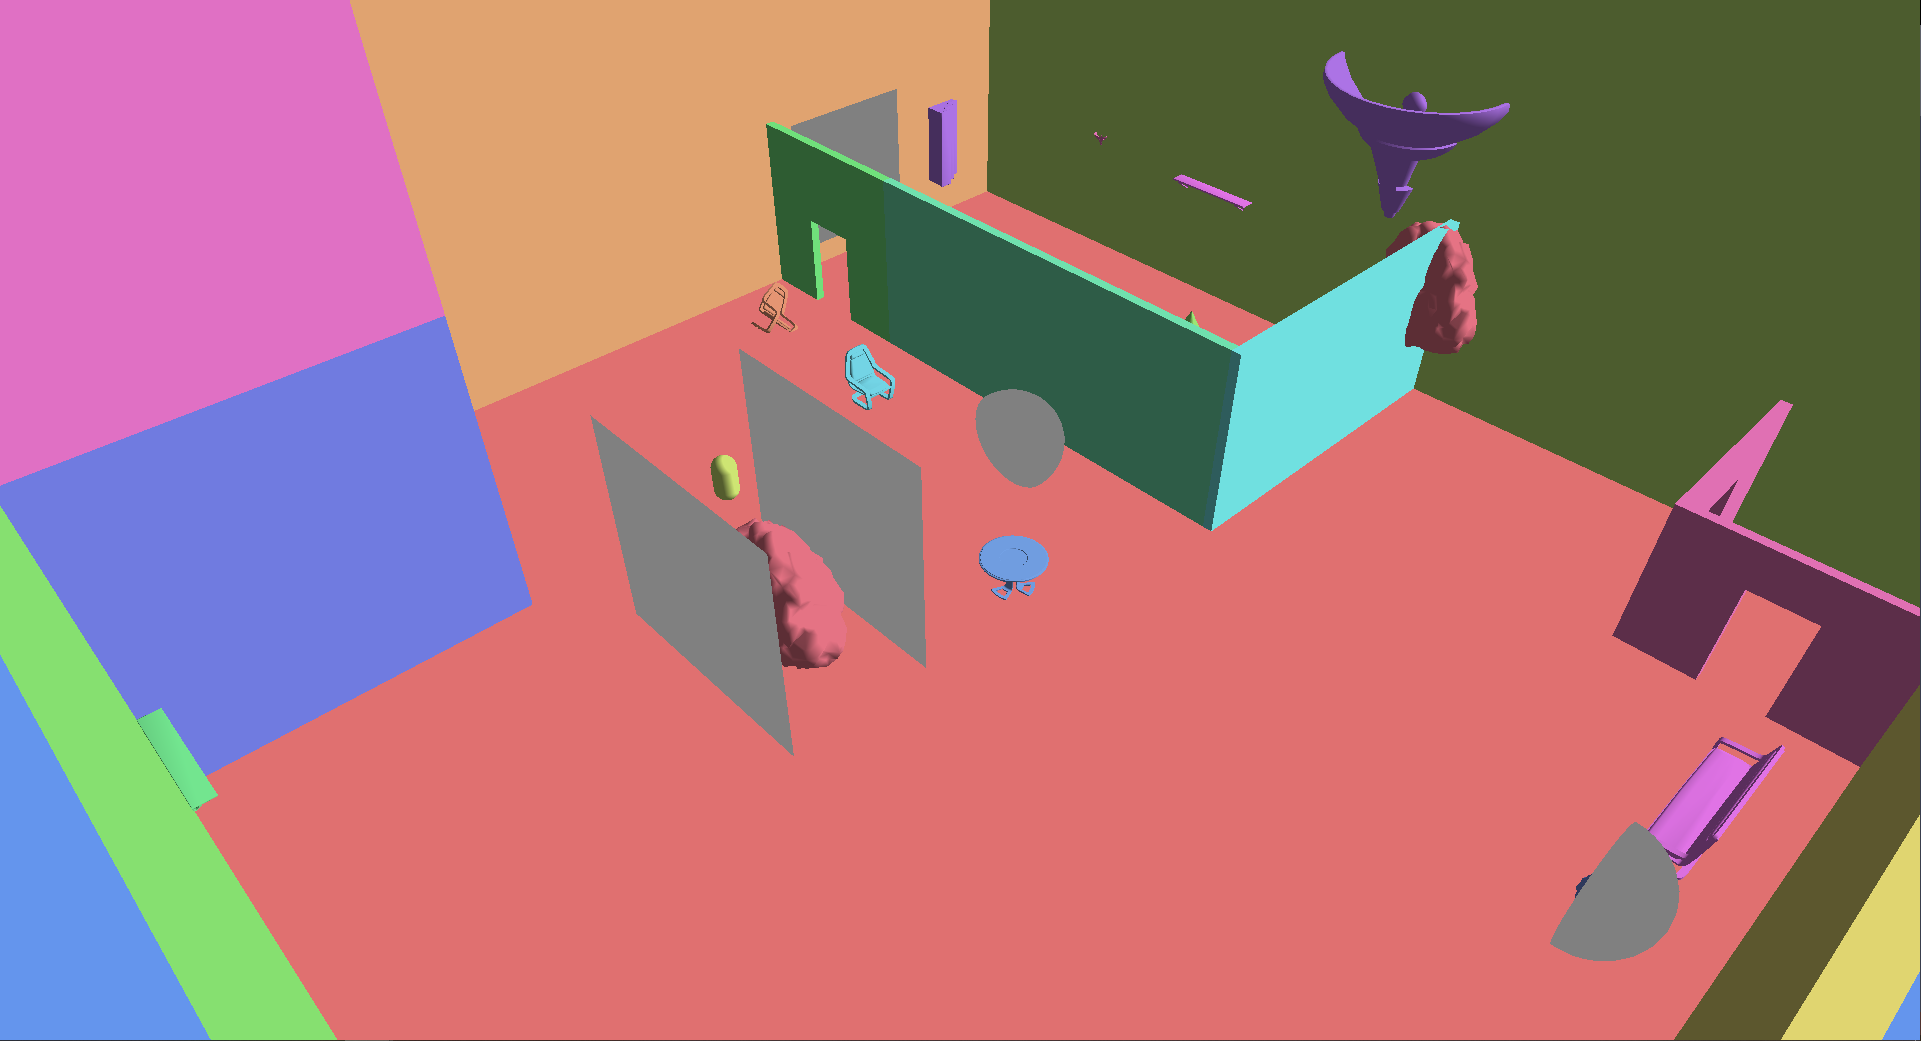
\includegraphics[width=\linewidth]{images/portals.png}
	\caption{Demo scene with no recursions}
	\label{fig:demodisabled}
\end{figure}


Figure~\ref{fig:demodisabled} shows the demo scene. The \gls{recursioncount} was to 0, essentially disabling the portals. They are displayed in grey, which is the colour indicating reaching the maximum recursion count. Note that a portal's transform and shape can be completely arbitrary.

\subsection{Recursions}

\begin{figure}[H]
	\centering
	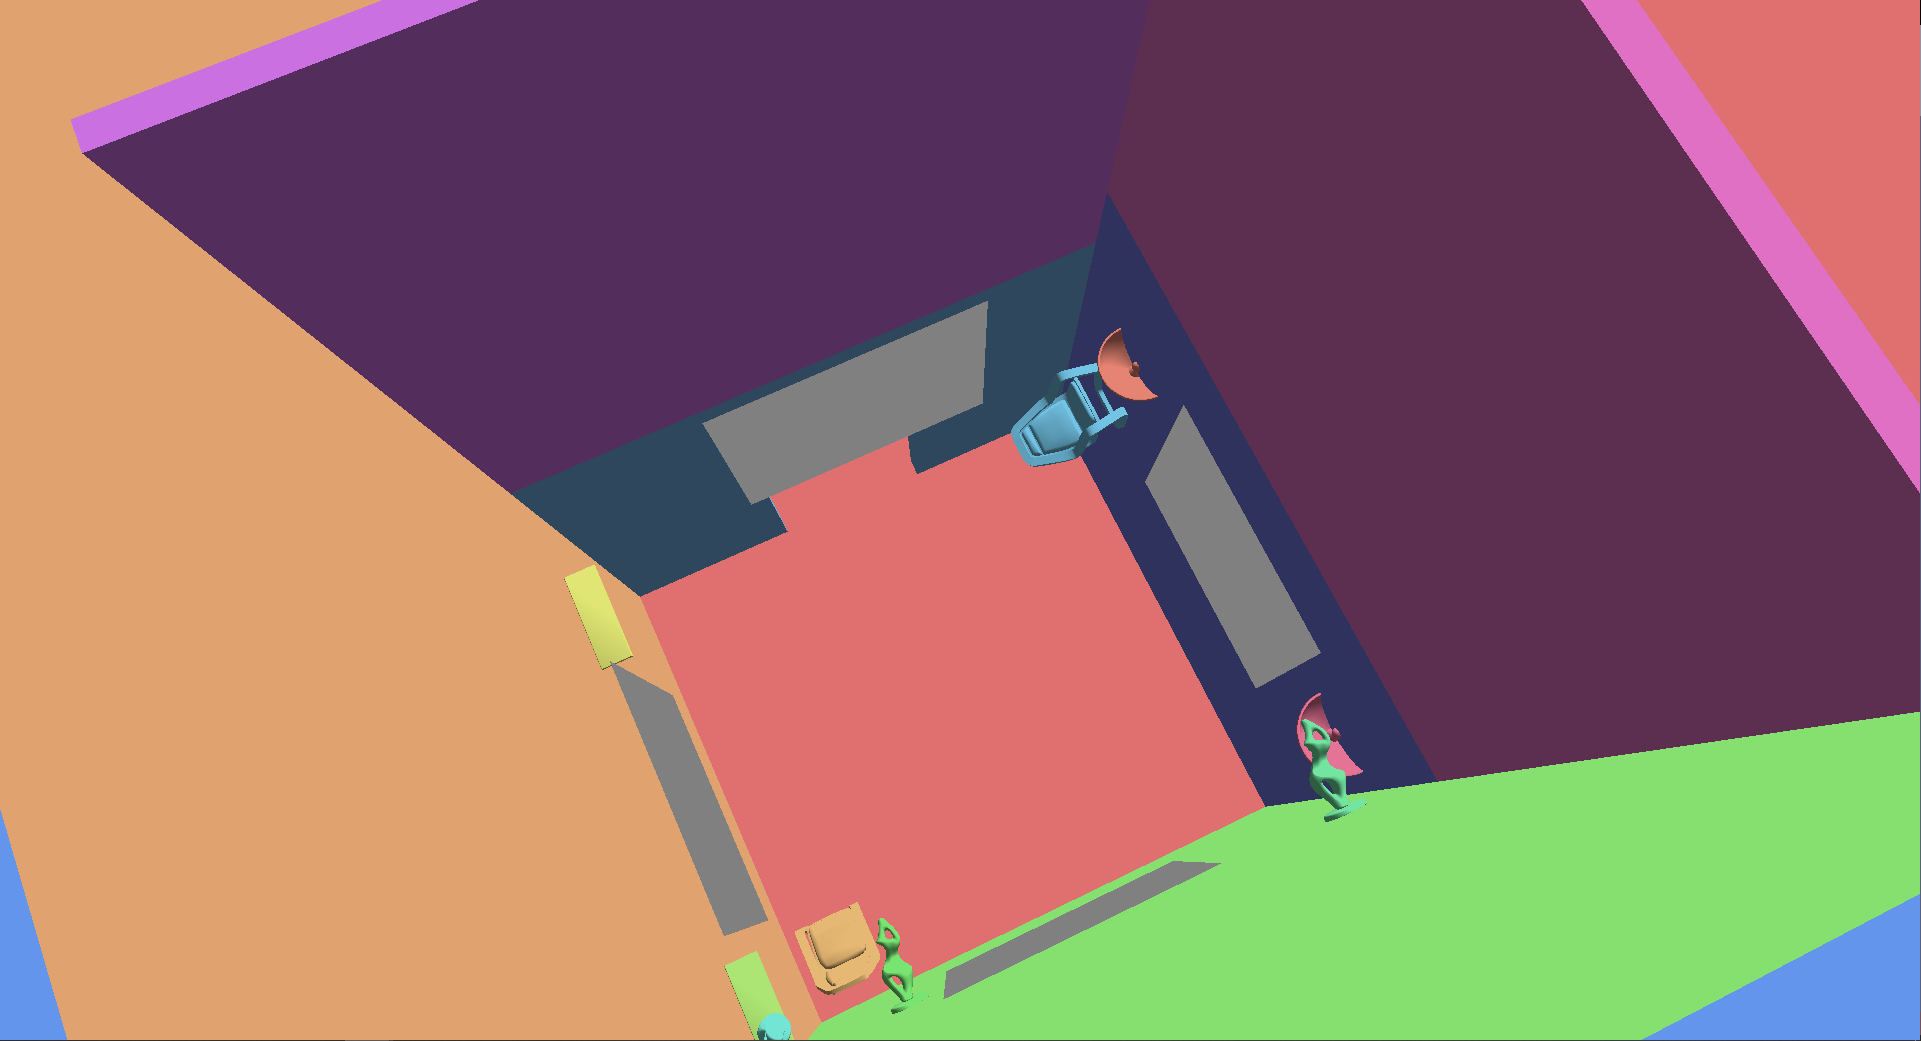
\includegraphics[width=\linewidth]{images/room.png}
	\caption{A room seen from the top, with recursion count 0}
	\label{fig:roomlayout}
\end{figure}

Figure~\ref{fig:roomlayout} shows a room within the scene from the top with disabled portals. The top and the left portals form one portal pair, while the bottom and the right portal form another portal pair.

\begin{figure}[H]
	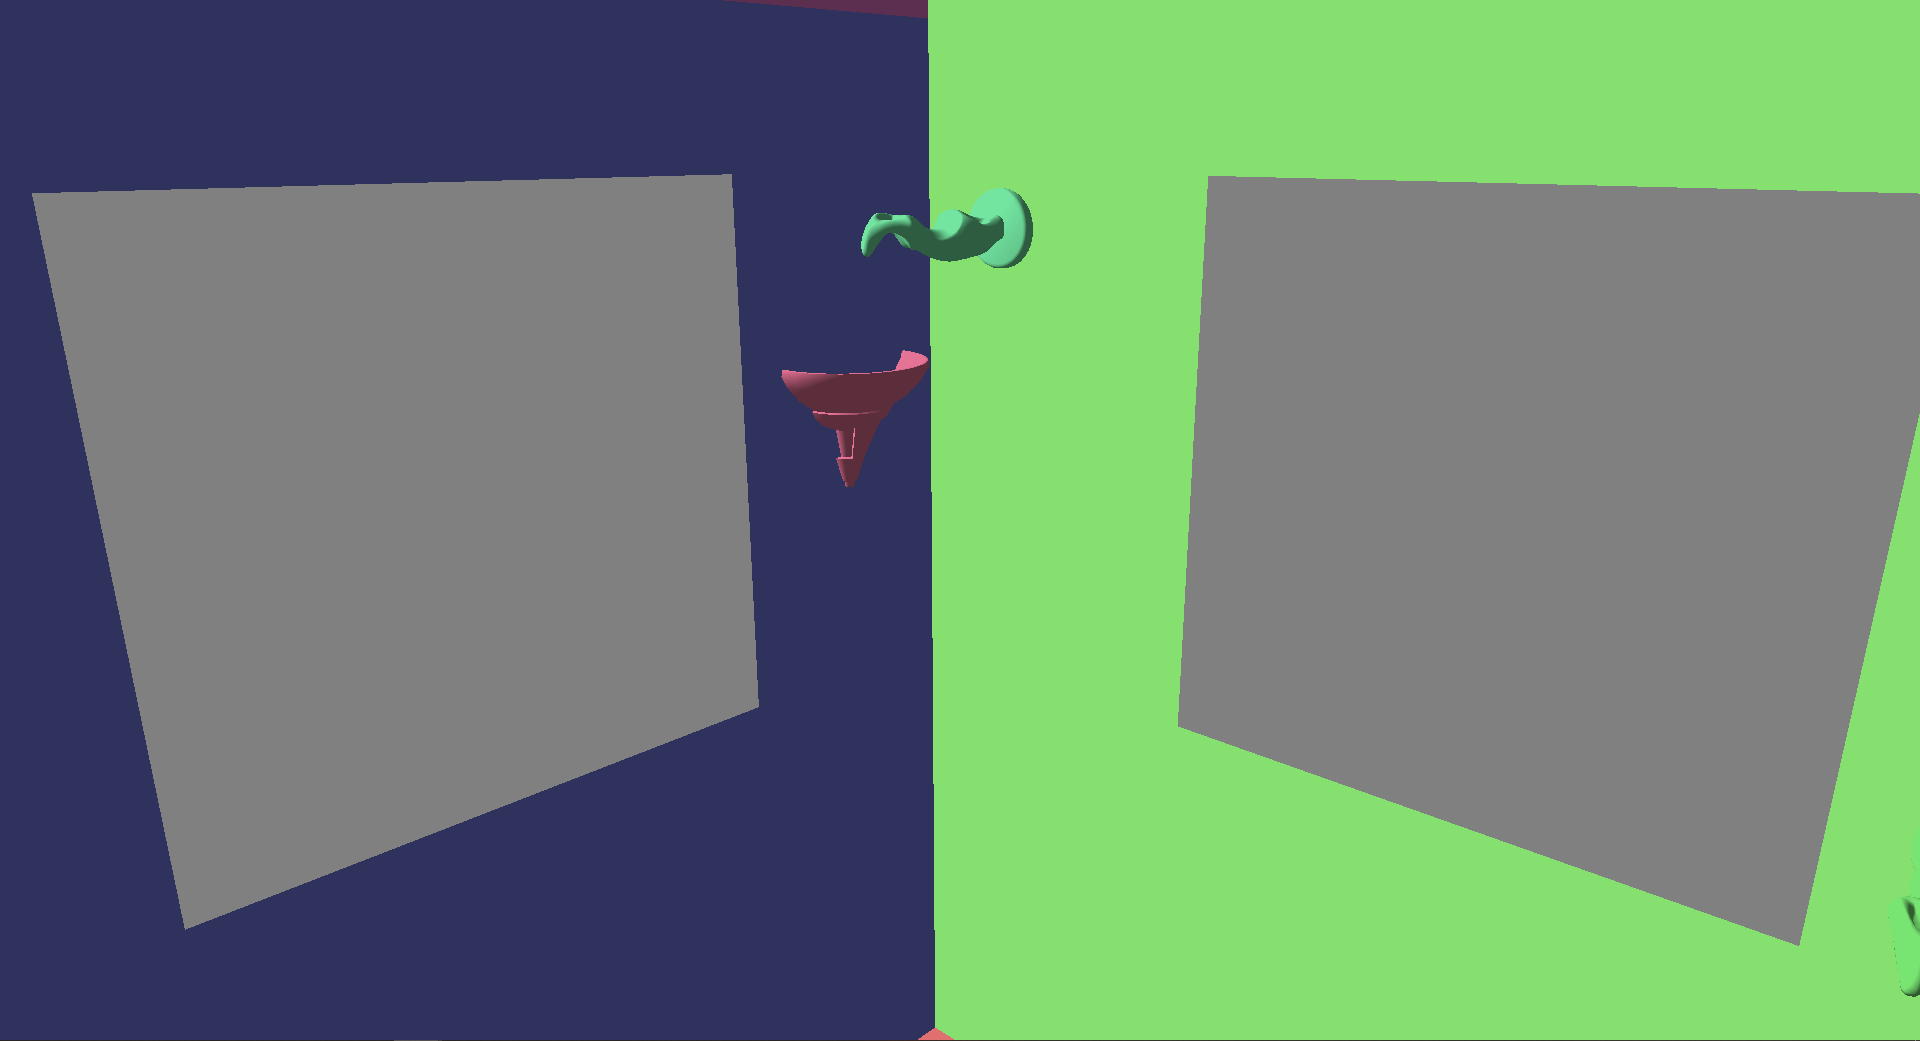
\includegraphics[width=\linewidth]{images/roomportalsr0.png}
	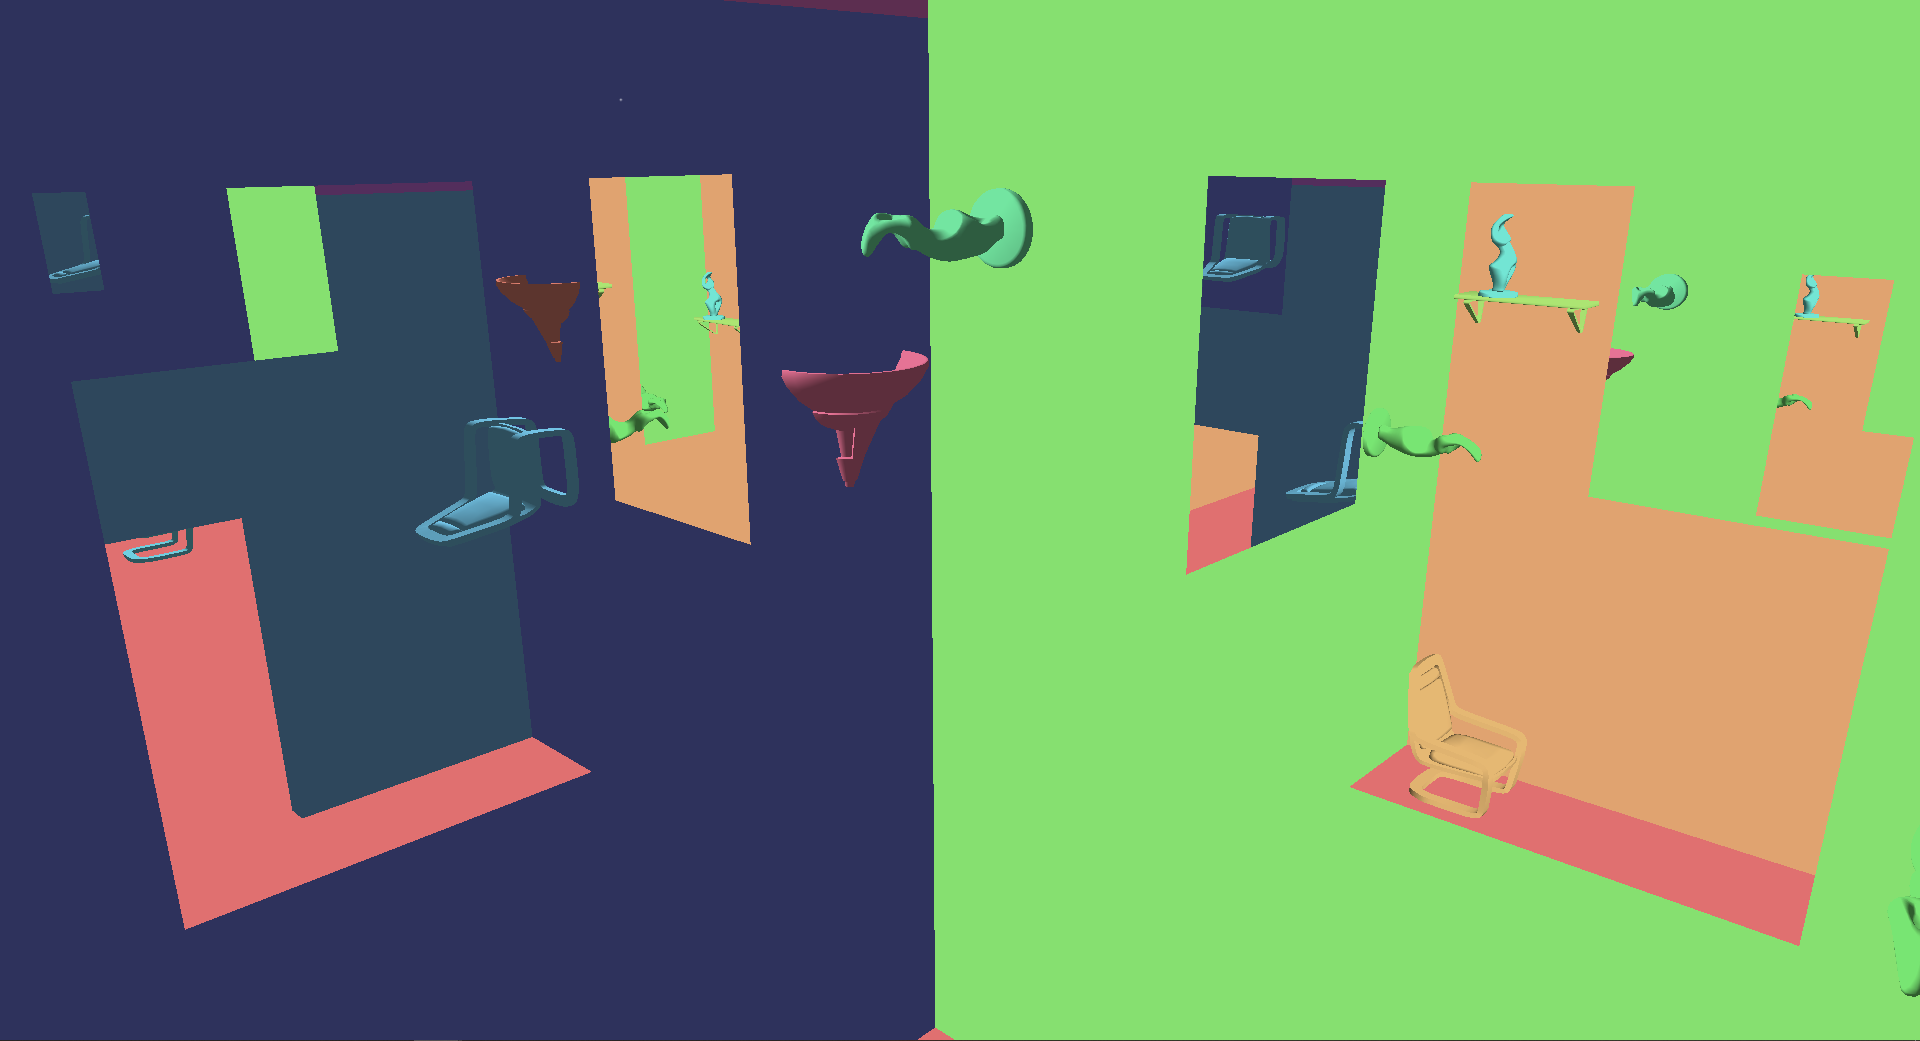
\includegraphics[width=\linewidth]{images/roomportals.png}
	\caption{Another viewpoint of the room. The top picture is with recursion count of 0, the bottom with a recursion count of 4}
	\label{fig:room}
\end{figure}


Figure~\ref{fig:room} shows the same room as figure~\ref{fig:roomlayout}, but from a different viewpoint. The top image has a \gls{recursioncount} of 0, while the bottom one has a \gls{recursioncount} of 4. Note that the orange and brighter bluish coloured walls cannot be seen without the portals. On the right side multiple recursion can be seen. The green and orange wall are alternating. This indicates that more than one portal pair is involved in the recursion.

\subsection{Non-Planar Portals}
\label{section:nonplanar}

This section showcases portals, that are defined by half-spheres. It shows that the prototype works with non-planar portals.

\begin{figure}[H]
	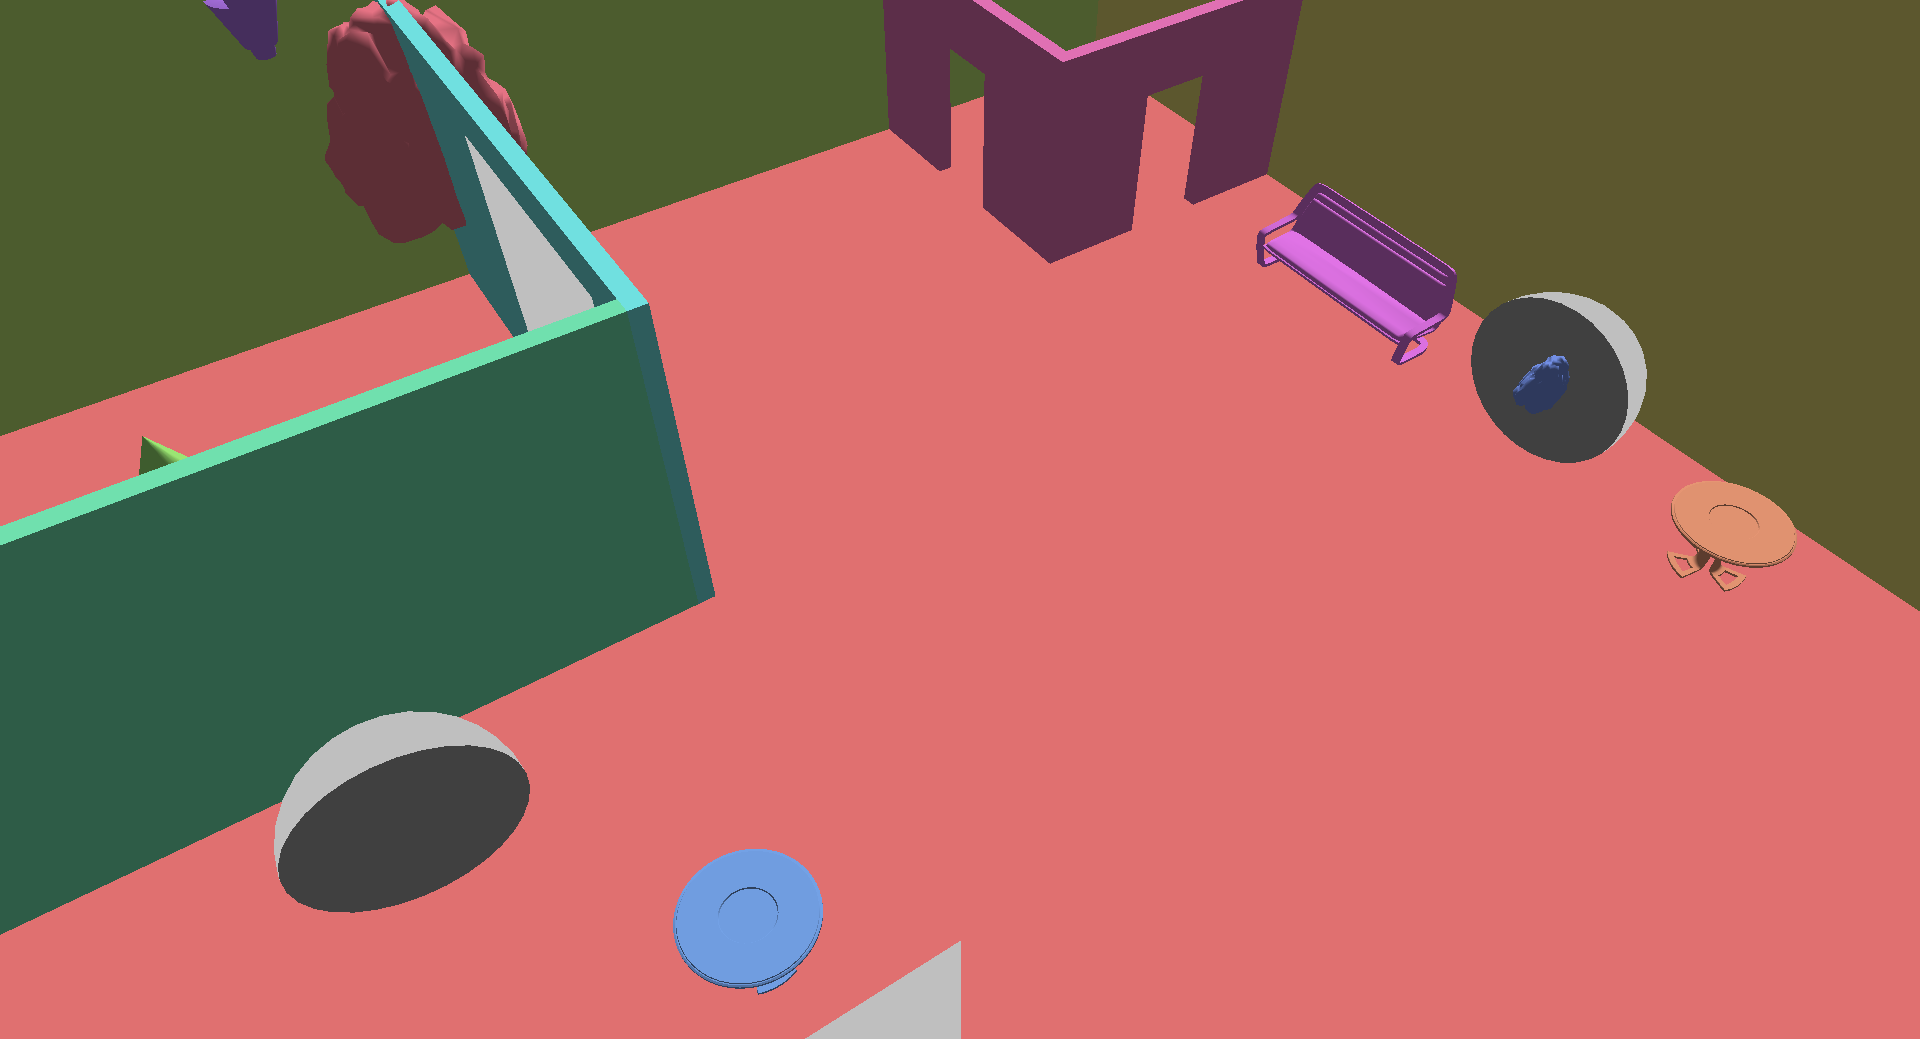
\includegraphics[width=\linewidth]{images/nonplanarlayout.png}
	\caption{The two half-sphere portals and their surroundings}
	\label{fig:nonplanarlayout}
\end{figure}

Figure~\ref{fig:nonplanarlayout} shows the two half-sphere portals and their surroundings. The half-spheres' front faces are in light grey, while their back faces are in dark grey. Notice that the blue rock on the right side is inside the half-sphere and can be seen through its opening.

\begin{figure}[H]
	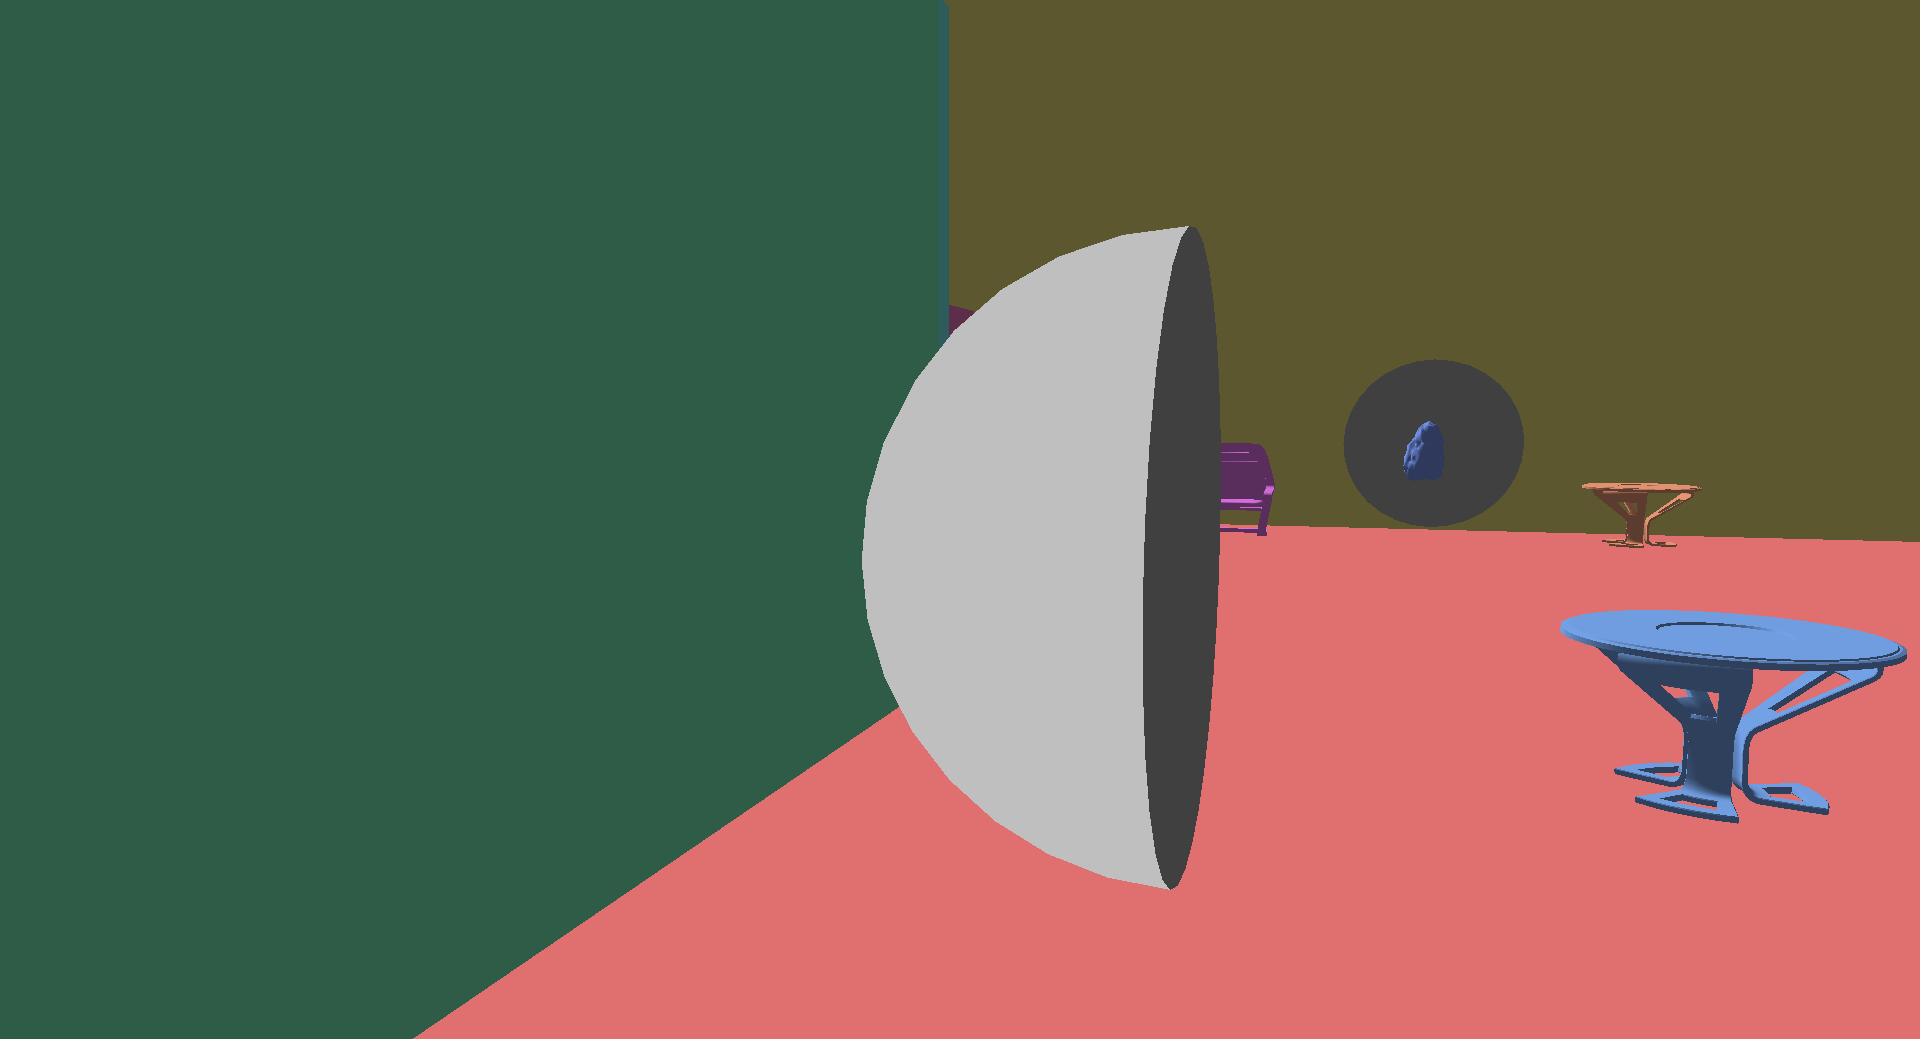
\includegraphics[width=\linewidth]{images/NonPlanarR0.png}
	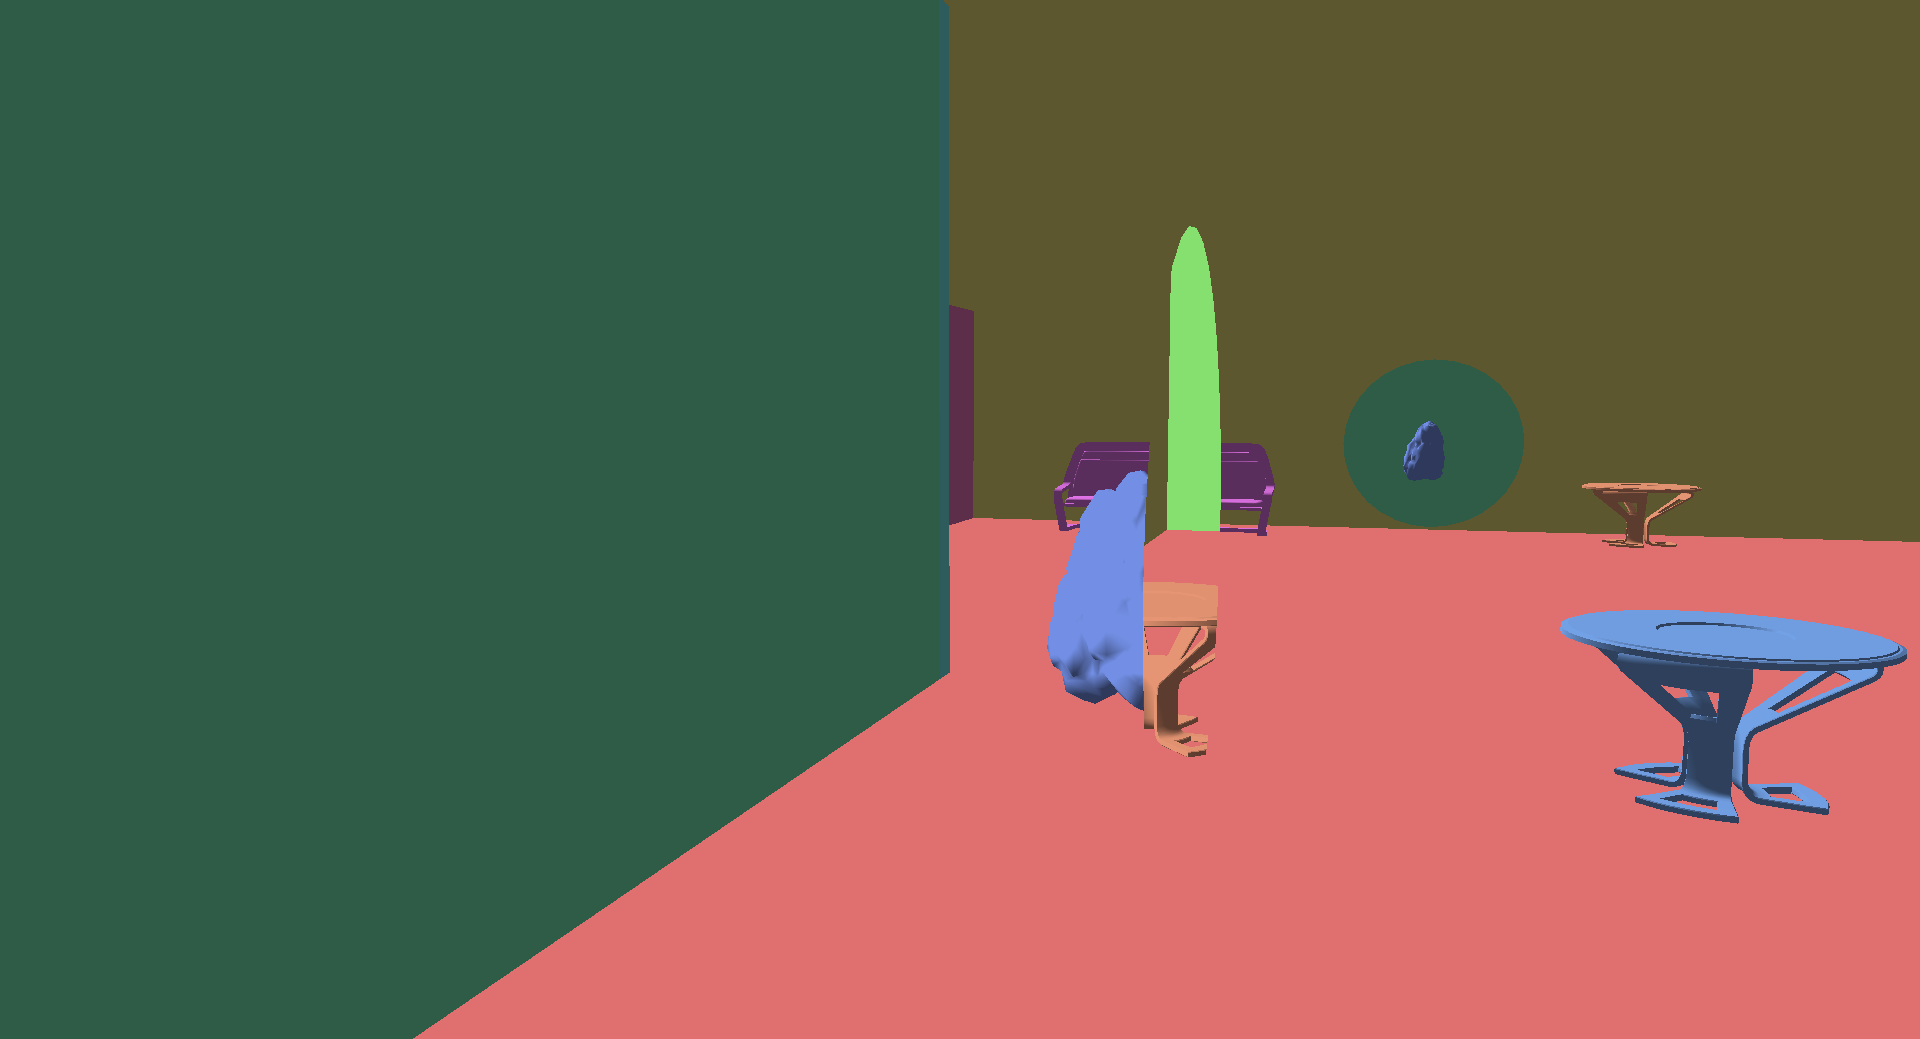
\includegraphics[width=\linewidth]{images/nonplanar.png}
	\caption{The two half-sphere portals. The top picture is with recursion count of 0, the bottom with a recursion count of 4}
	\label{fig:nonplanar}
\end{figure}

Figure~\ref{fig:nonplanar} shows the same two half-sphere portals from another viewpoint. The top picture is with a recursion count of 0, the bottom with a recursion count of 4. In this picture the light grey colour not only indicates the portals front face, but also which pixels needed two recursions for their colour in the bottom picture. At the dark grey pixels one recursion only one recursion is needed. The front half-sphere portal will be referred as \gls{endpoint} A and the back half-sphere portals as \gls{endpoint} B.

Notice that in the bottom picture more parts of the purple bench behind the \gls{endpoint} A are visible. The two portal cancel each other out. Additionally, parts of the blue rock which is inside \gls{endpoint} B can be seen. The contents of \gls{endpoint} A and B appear swapped. When looking through the hole in \gls{endpoint} A, the orange table next to \gls{endpoint} B can be seen. Inside \gls{endpoint} B a green colour can be seen, which is the same colour as the one from the wall next to \gls{endpoint} A.

\section{Implementation Performance}
\label{section:performancemeasurement}

This section covers performance measurements, to test the prototype's suitability for real time applications. Additionally, bottlenecks can be discovered, providing insights on how the prototype can be improved in the future.

\subsection{Measuring method}
All tests are run on the same machine. It runs on Microsoft Windows 10 Education (10.0.18362). It uses the AMD Ryzen 7 1700 as \gls{cpu} and the Radeon RX 570 as \gls{gpu}.

In this test measures the time taken to render one frame. This includes the time the \gls{cpu} needs to prepare the data for the \gls{gpu} (e.g. calculating camera matrices) as well as recording the command buffer. The time is measure in milliseconds using C++'s chrono library. The time is measured for 128 consecutive frames. The average, median, minimum and maximum time of the measured times are printed to the console.


The measured milliseconds differ depending on the view. Multiple viewpoints were measured. Multiple recursion counts and maximum visible portals are measured. The recursions are noted in the form X-Y-Z, where X corresponds to the maximum visible portals in recursion 0, Y to maximum visible portals in \textit{recursion 1} and so forth. For example, 8-6-4 indicates a recursion count of 3, using 8 maximum visible portals in recursion 0, 6 in \textit{recursion 1}, and 4 in recursion 2. The last recursion always has a count of 0, as nothing will be drawn inside the portals. 

\iffalse

The following configurations were tested. 
\begin{itemize}
	\item No Recursions
	\item 8-6-4-2
	\item 8-6-4
	\item 8-6
	\item 8
	\item 12-12-12-12
	\item 12-12-12
	\item 12-12
	\item 4
	\item 4-4-4-4
	\item 4-4-4
	\item 4-4
	\item 4
	
\end{itemize}
\fi

\subsection{Demo Scene Render Baseline}
The tests in this section all use the same scene. It contains 6 portal pairs which are 12 portals in total. This number is important, as it dictates how many view matrices need to be calculated.


\begin{table}[H]
	\centering
	\begin{tabular}{|l|l|l|l|l|l|l|}
		\hline
		Test Case    & Average & Median & Min   & Max   & Relative Median \\ \hline
		No Recursion & 1.03    & 0.99   & 0.98  & 1.37  & 0.99            \\ \hline
		0            & 1.57    & 1.56   & 1.55  & 1.70  & 0.57            \\ \hline
		0-0          & 2.14    & 2.14   & 2.12  & 2.19  & 0.58            \\ \hline
		0-0-0        & 2.91    & 2.91   & 2.79  & 3.00  & 0.77            \\ \hline
		0-0-0-0      & 6.51    & 6.56   & 6.01  & 6.95  & 3.65            \\ \hline
		0-0-0-0-0    & 41.75   & 41.86  & 40.75 & 44.66 & 35.30           \\ \hline        
	\end{tabular}
	\caption{Time to render a frame in milliseconds, without an object on screen and max visible portal count set to 0}
	\label{tab:baseline}
\end{table}

Table~\ref{tab:baseline} shows the render time for different recursion counts with max visible portals always set to zero in milliseconds. This represents the time that is needed to calculate the view matrices and submit the render commands with instance counts of 0. The number of render commands scales linearly with recursion count, while the number of camera matrices to generate scales super-linearly. The time to render for four and five recursions is significantly higher compared to their previous recursion. This probably indicates that the render time for these cases is dominated by the time to calculate the camera matrices and sending them to the \gls{gpu}.

\subsection{Demo Scene View Matrix Calculation}
\label{section:perfmatrixcalc}

\begin{table}[H]
	\centering
	\begin{tabular}{|l|l|l|l|l|}
		\hline
		Recursions & Average & Median  & Min     & Max     \\ \hline
		1          & 0.36    & 0.36    & 0.34    & 0.37    \\ \hline
		2          & 4.70    & 4.75    & 4.48    & 4.76    \\ \hline
		3          & 56.47   & 56.72   & 55.00   & 57.13   \\ \hline
		4          & 678.44  & 670.10  & 649.83  & 691.08  \\ \hline
		5          & 8,204.14 & 8,209.05 & 7,997.10 & 8,305.70\\ \hline
	\end{tabular}
	\caption{Time in microseconds to calculate the camera matrices for 12 portals}
	\label{tab:cameramatricecalc}
\end{table}

\begin{table}[H]
	\centering
	\begin{tabular}{|l|l|l|l|l|}
		\hline
		Recursions & Average   & Median  	& Min     	& Max        \\ \hline
		1          & 0.91      & 0.92		& 0.87    	& 0.93       \\ \hline
		2          & 11.28     & 11.34		& 11.00    	& 11.40      \\ \hline
		3          & 133.46    & 134.65		& 126.88   	& 136.69     \\ \hline
		4          & 1,565.47  & 1,568.29	& 1,510.01  & 1,642.43   \\ \hline
		5          & 18,752.38 & 18,717.63	& 1,8313.85 & 19,266.95 \\ \hline
	\end{tabular}
	\caption{Time in microseconds to calculate the view matrices for 12 portals}
	\label{tab:cameramatricecalcinverse}
\end{table}

Table~\ref{tab:cameramatricecalc} shows the time needed to calculate just the camera matrices. Note that microseconds were as the unit. Table~\ref{tab:cameramatricecalcinverse} shows the total view matrix calculation, which is first calculating the camera matrices and then inverting them. This takes roughly three times longer, compared to just calculating the matrices. Inverting makes up for approximately two thirds of the total calculation time.

However, both tables show that calculating the view matrices takes a significant portion of the base render time. With four recursions it is approximately 23\% of the total time, for five recursions approximately 44\%. 

\subsection{Demo Scene Render Performance - Empty View}


\begin{table}[H]
	\centering
	\begin{tabular}{|l|l|l|l|l|l|}
		\hline
		Test Case   & Average & Median & Min    & Max    & Relative Median \\ \hline
		8           & 1.56    & 1.53   & 1.51   & 1.95   & -0.03           \\ \hline
		8-6         & 2.09    & 2.09   & 1.99   & 2.20   & -0.05           \\ \hline
		8-6-4       & 6.80    & 6.81   & 5.90   & 7.65   & 3.9             \\ \hline
		8-6-4-2     & 16.51   & 16.48  & 14.67  & 17.79  & 9.92            \\ \hline
		12          & 1.62    & 1.59   & 1.50   & 2.14   & 0.03            \\ \hline
		12-12       & 4.47    & 4.45   & 3.64   & 5.29   & 2.31            \\ \hline
		12-12-12    & 47.63   & 47.58  & 46.35  & 49.11  & 44.67           \\ \hline
		12-12-12-12 & 559.65  & 559.57 & 557.29 & 561.59 & 553.01          \\ \hline
		4           & 1.57    & 1.53   & 1.50   & 2.23   & -0.03           \\ \hline
		4-4         & 2.15    & 2.09   & 2.05   & 2.90   & -0.05           \\ \hline
		4-4-4       & 2.76    & 2.76   & 2.59   & 2.92   & -0.15           \\ \hline
		4-4-4-4     & 9.14    & 9.15   & 7.50   & 10.94  & 2.59            \\ \hline
	\end{tabular}
	\caption{Time in milliseconds to render a scene with 12 portals without an object on screen, as well as the relative median time compared to table~\ref{tab:baseline}}
	\label{tab:rendernothing}
\end{table}


Table~\ref{tab:rendernothing} shows multiple measurements taken for rendering no visible geometry or portal. The image will correspond to the clear colour. The time is measured in milliseconds. In addition, it shows the relative median time compared to the median time of table~\ref{tab:baseline}. The relative median time is sometimes negative. This likely is due to other programs running in the background during the test.

This table indicates that not only the recursion count, but also the number of maximum visible portals matter significantly. If the visible portal count is low enough, rendering with additional recursions can still be faster than with higher visible portal counts and less recursions. Rendering all portals, in this case 12 portals, every recursion is similar to the first approach to portal rendering described in section~\ref{section:intialimplementation}. In this case only two recursions can be used for real-time applications. Otherwise the prototype would not even reach 30 \gls{fps}. This means that the maximum portal count of the initial portal rendering approach was not only limited by the stencil buffer bits. It was also limited by its performance. Being able to configure visible portals counts is significant.

Lastly, the table indicates that for this implementation the maximum recursion count is 4 for real time applications. However, with 4 recursions the scene needs to be well designed, so that the maximum visible portal count can be kept low.




%% The value of table~\ref{tab:renderrelative} plus the value of table~\ref{tab:baseline} would 


\subsection{Demo Scene Render Performance - Regular View}
\label{section:renderperformance}

Render times without any rendered object, may make for good baselines, but do not indicate how the prototype behaves in real cases. 

\begin{figure}[H]
	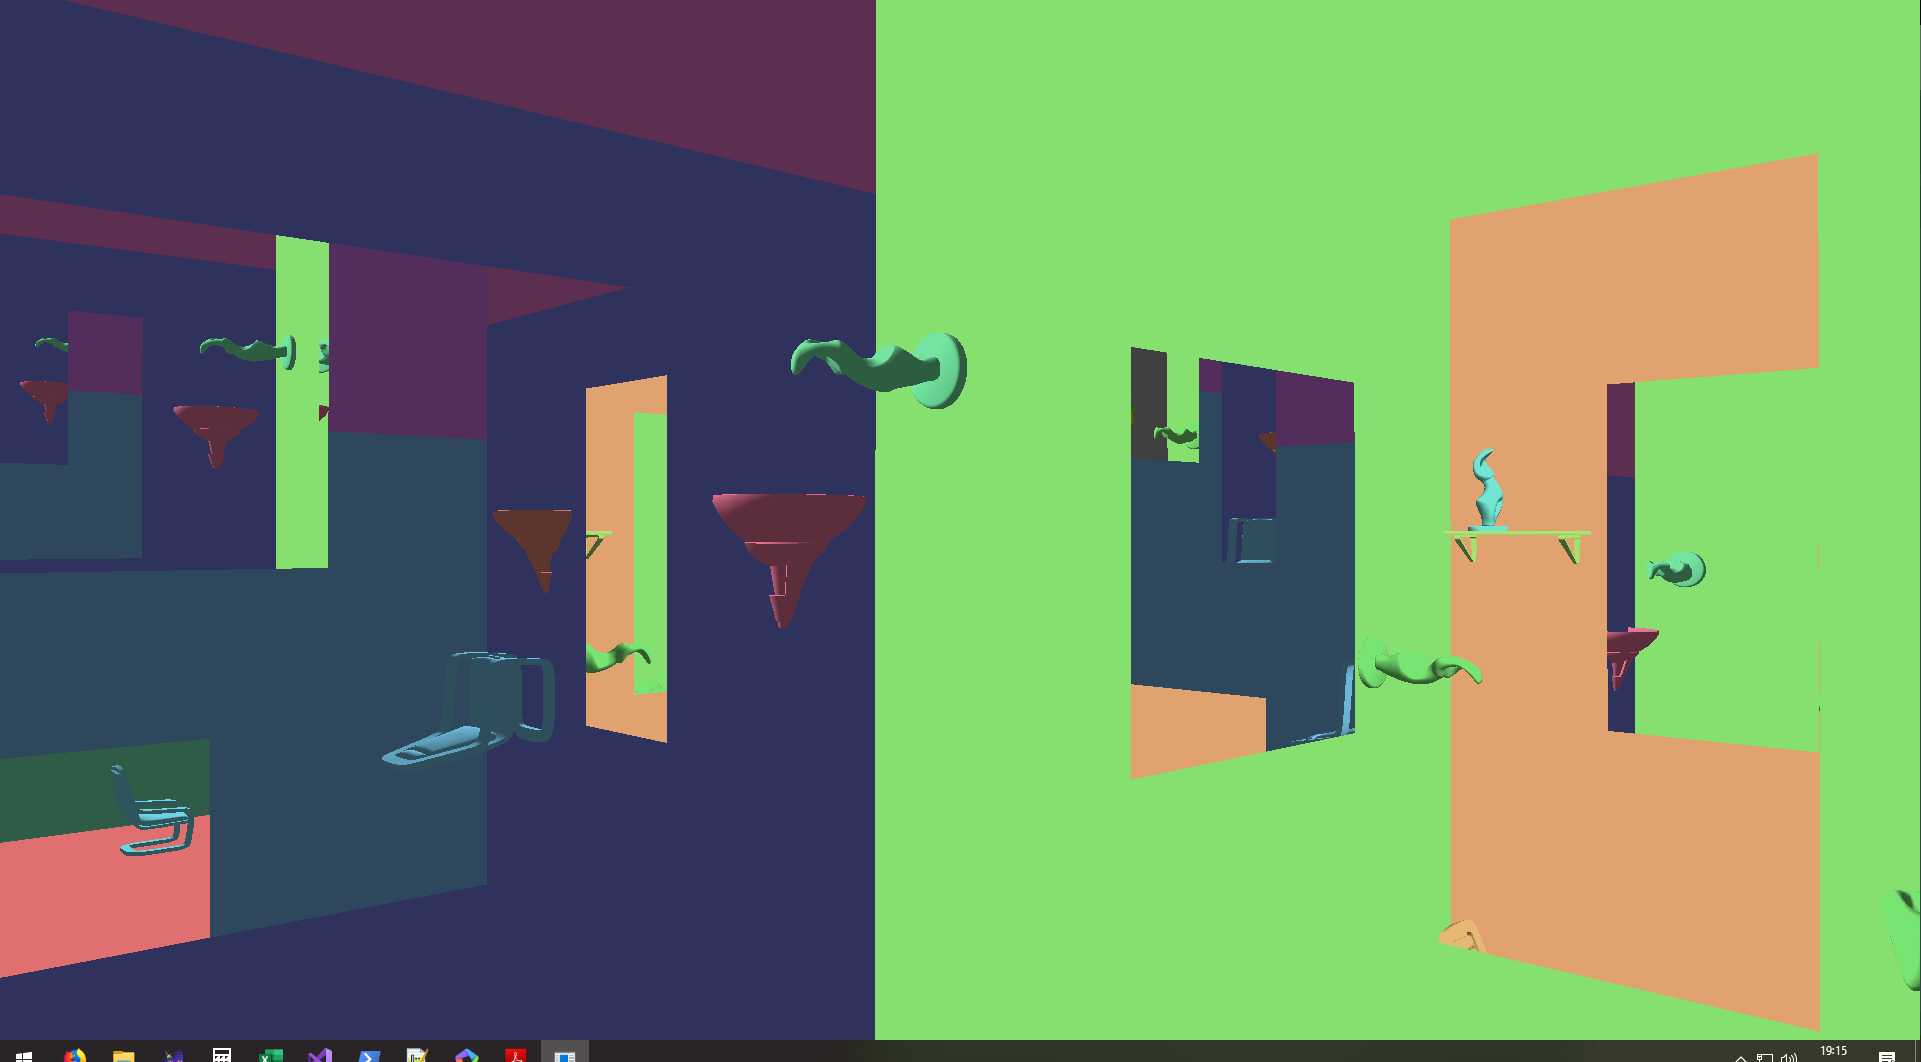
\includegraphics[width=\linewidth]{images/testsnapshot.png}
	\caption{The  viewpoint for measuring. Maximum visible portal and recursion count to produce the image was 8-6-4-2.}
	\label{fig:perfviewpoint}
\end{figure}

Figure~\ref{fig:perfviewpoint} shows the viewpoint of the following measurement. There are two visible portals and a few recursions. While scenes with many more visible portals could be constructed, this serves as a reasonable case. Note that the displayed image does not look the same for all measurements. Some test cases will only show one recursion.

\begin{table}[H]
	\centering
	\begin{tabular}{|l|l|l|l|l|l|}
		\hline
		Test Case   & Average & Median & Min    & Max    & Relative Median \\ \hline
	   %No Recursion& 1.17    & 1.16   & 1.15   & 1.33   & 0.17		   	   \\ \hline
		8           & 2.95    & 2.90   & 2.24   & 3.48   & 1.37            \\ \hline
		8-6         & 8.29    & 8.28   & 7.36   & 8.96   & 6.19            \\ \hline
		8-6-4       & 14.85   & 14.84  & 13.96  & 15.99  & 8.03            \\ \hline
		8-6-4-2     & 24.97   & 24.91  & 23.09  & 27.05  & 8.43            \\ \hline
		12          & 3.02    & 2.98   & 2.36   & 3.51   & 1.39            \\ \hline
		12-12       & 10.76   & 10.75  & 9.99   & 11.56  & 6.30            \\ \hline
		12-12-12    & 55.21   & 55.20  & 54.32  & 56.25  & 7.62            \\ \hline
		12-12-12-12 & 568.21  & 568.20 & 566.05 & 569.51 & 8.63            \\ \hline
		4           & 2.84    & 2.79   & 2.06   & 3.41   & 1.26            \\ \hline
		4-4         & 6.08    & 6.07   & 5.17   & 6.79   & 3.98            \\ \hline
		4-4-4       & 9.45    & 9.45   & 8.08   & 10.48  & 6.69            \\ \hline
		4-4-4-4     & 16.97   & 16.99  & 15.04  & 19.33  & 7.84            \\ \hline
	\end{tabular}
	\caption{Time in milliseconds to render a scene with 12 portals from Figure~\ref{fig:perfviewpoint}'s viewpoint, as well as the relative median time compared to render times without objects on the screen.}
	\label{tab:perfviewpoint}
\end{table}

Table~\ref{tab:perfviewpoint} shows the render times in milliseconds for the image shown in figure~\ref{fig:perfviewpoint}. The last column is the increase in median the render times compared to table~\ref{tab:rendernothing}, which showed no objects on the screen. The median is significantly higher, compared to table~\ref{tab:rendernothing}. This is especially true for the low recursion measurement. Their median render time increase makes up significant fractions of their total median render time. This makes sense, as the most objects are only rendered for the first recursion. For later recursions, it is less likely that an object needs to be drawn. This indicates that producing degenerate triangles for objects that do not need to be rendered (see section~\ref{section:viewmatrixselection}), improves performance. However, this also shows that the base render times from table~\ref{tab:rendernothing} are not too reliable. The actual render times depend heavily on the rendered scene. This table alone shows render times up to 4 times more than the baseline (Test Case 8-6). Care needs to be taken when building scenes. The numbers also suggest that the \gls{recursioncount} should likely be limited to 3 instead of the previous stated 4.


\section{Properties of Watertight Portals}
\label{section:watertight}
Special properties of watertight portals were found while testing the prototype. Watertight portals are portals that use a watertight mesh. When looking at a watertight portal, objects behind it will be visible. Watertight portals seem as though they do not exist. However, their contents are swapped.

\begin{figure}[h]
	\centering
	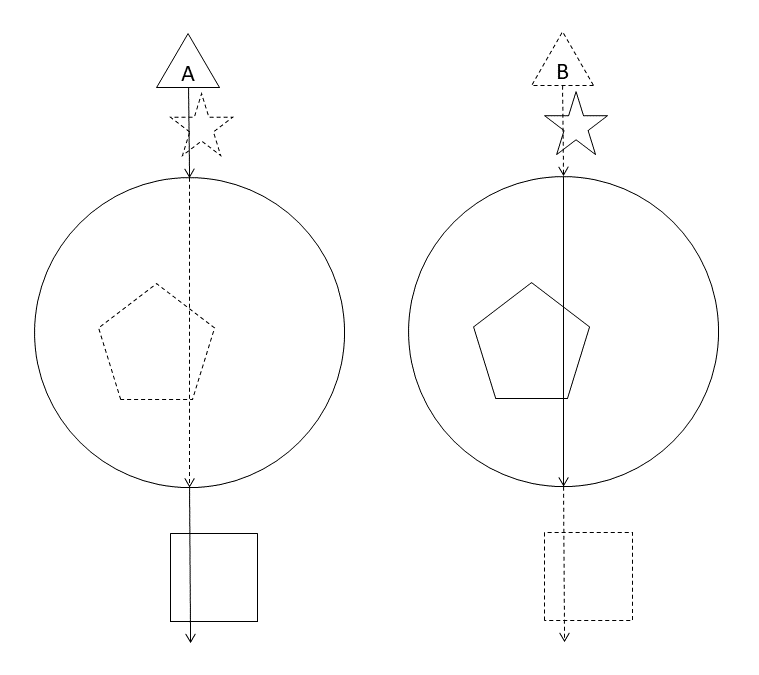
\includegraphics[width=0.8\linewidth]{images/watertight.png}
	\caption{A watertight portal pair}
	\label{fig:watertightportals}
\end{figure}

Figure~\ref{fig:watertightportals} show an example of a watertight portal pair. The two big spheres are the two endpoints of a watertight portal pair. There are two viewpoints A and B.
There are two approaches to interpret the figure, which both are valid.

The first is that A's \gls{viewray} is indicated by full stroked arrows, while B's \gls{viewray} is indicated by doted arrows. Only objects with full strokes can be seen. The \gls{viewray} teleports when passing through the portal, and teleports back when passing it again. This is how the view is rendered.

The other is that A and B's \gls{viewray} is a not teleported. When the \gls{viewray} is fully stroked only fully stroked objects are visible. When the \gls{viewray} is dotted only dotted objects are seen. This is how the view looks for the user.

In this example A can only see the pentagon and the square, while B can only see the star. Only the fully stroked objects are the actual placements of the object. Notice that it looks, as if both spaces were swapped.

When using Watertight portals, they need to be created or transformed during runtime, otherwise they just impact performance without any gain. After discovering this fact, the watertight portals were removed from the prototype's scenes.

However, this property of watertight portals could be exploited. If watertight portals are treated differently compared to regular portals, there might be some opportunities for optimization.

\subsection{Holes}
Cutting holes inside an otherwise watertight portal has some interesting properties. As previously mentioned, a watertight portal is not really detectable and only serves for switching spaces. However, when a hole is cut, the hole itself would look like a portal. The hole could be interpreted as an additional portal, which cancels out the watertight portal. But the watertight portal would not be visible to the user, so they see only that additional portal, which does not exist. This property can be seen in the half-sphere portals as shown in figure~\ref{fig:nonplanar} in section~\ref{section:nonplanar}. The dark grey area in the top image indicates the circular planar hole, which is the only part of the bottom picture which looks like a portal. The actual part of the half-sphere portal only serves as a border for the swapped space.
\chapter{Performance Improvements}
\label{section:performanceimprovements}

Section~\ref{section:performancemeasurement} measured the prototype's performance and discovered potential bottlenecks. This section will focus on how the performance could be further improved using this information. Then two additional potential performance improvements are discussed, which are not based on measurements.

\section{Preventing false Visible Portals}
\label{section:falsevisible}
The manual stencil test introduced in section~\ref{section:dynamicportalinstancerendering}, enabled stencil testing portals earlier. Portal fragments that fail the stencil test, no longer count as visible portals for the algorithm described in section~\ref{section:visibleportalcount}. However, unless it is \textit{recursion 0}, fragments that would fail the far depth test still count as visible. For subsequent recursions, the depth tests must to be performed after the shader, due to the manual stencil and near depth tests, which may discard a fragment. This can lead to false visible portals.

Table~\ref{tab:perfviewpoint} from section~\ref{section:renderperformance} has shown that there is quite a difference between rendering nothing and rendering multiple portal recursions. The less visible portals there are, the better the performance.

One way to prevent false visible portals is by running a depth pre-pass for the portals. This pass renders all portals but does nothing but write depth values. It still performs the manual tests, for stencil and near buffer. Then the portals are drawn again, with an early depth test. For this pass writes to the depth buffer can be disabled. Thus, the nearest depth values are already known and only portals that will not be occluded qualify as visible for the visible portal count algorithm.

There is also another possibility, which only needs an additional depth texture, but no pre-pass. While rendering objects a \gls{fardepthbuffer} is used, just as always. However, during the portal rendering, this depth buffer is given as input for the portal shaders. They perform an additional manual test for the far depth. Portals still use a regular depth buffer, so that portals occlude each other correctly. Although portals occluded by other portals still count as visible, portals occluded by objects do not. As the latter case is far more likely, this could reduce the number of false visible portals greatly.

\section{Camera Matrix Improvement opportunities}
In section~\ref{section:generatingviewmatrices} it was found that generating view matrices takes a considerable amount of time. In the following sections three possible improvements are discussed.

\subsection{Remove Matrix Inversions}
Currently when calculating the view matrices, first all camera matrices are calculated. Next, each of them is inverted to find the view matrices. $C_n$ is the n\textsuperscript{th} \gls{cameramatrix}, $T_n$ is the n\textsuperscript{th} teleport matrix and $V_n$ is the n\textsuperscript{th} view matrix. $C_0$ is the initial \gls{cameramatrix}. This can be written as:

$$C_n = T_{n} * C_{n-1}$$
$$V_n = (C_{n})^{-1}$$

Section~\ref{section:perfmatrixcalc} has shown that calculating the inverse of the matrices is responsible for approximately two thirds of the total calculation time. The new approach would not need to take the inverse of a matrix. Instead the view matrices can be used directly.
Combining the previous two equations yields:

$$V_n = (T_n * C_n)^{-1} = C_n^{-1} * T_n^{-1}$$

The inverse camera matrices can be substituted by their respective view matrices.
$$V_n = V_{n-1} * T_n^{-1}$$

Results from previous calculation can be reused, the same way as previously. As the inverse of \gls{endpoint} A's teleportation matrix is equal to \gls{endpoint} B's teleportation matrix, no matrix but the initial \gls{cameramatrix} needs to be inverted. If time had permitted it, this optimization would definitely be included in the prototype.

\subsection{Excluding the initial view matrix}
\label{section:noveiw}
Let $Vwv0_n$ be the view matrix for portal n, which was not multiplied with the initial view matrix. Formally:

$$V_n = V_0 * Vwv0_n$$

$Vwv0_n$ can be defined recursively as:

$$Vwv0_n = Vwv0_{n-1} * T_n^{-1}$$

The advantage of leaving out $V_0$ from the multiplication is that, if all $T$ are constant all $Vwv0$ will be constant as well. These matrices would only need to be calculated once, instead of every frame. The final calculation to get the real view matrix can be done in the shader. This does not need to be a matrix multiplication, as it the view matrix is used only once in the shader for calculation a vertex's position. The two matrices can be multiplied consecutively with the vertex position, requiring less multiplications.

An array of these matrices could reside in \gls{gpu} local memory, as they do not need to be changed. Even for scenes with moving portals, this could be a useful optimization, as only the parts that depend on the moved portal need to be recalculated. However, whether this improves performance for a specific implementation needs to be tested.

\subsection{Calculating on the GPU}
Instead of calculating the view matrices on the \gls{cpu}, they could also be calculated on the \gls{gpu}.
This saves the \gls{gpu} bandwidth, as only the \glspl{teleportationmatrix}  and the camera's \gls{viewmatrix} need to be transferred, instead of an array of every possible permutation of portals. Additionally, the indirection described in section~\ref{section:viewmatrixselection} would not be needed anymore and could be removed. After the previous visible portal calculation, the \gls{viewmatrix} can be calculated and written to the correct location. Lastly, access is faster as the matrices are in \gls{gpu} local memory.

The total number of calculated matrices might be more or less on the \gls{gpu} compared to calculating it on the \gls{cpu}. This depends on the number of portals on the scene, the number recursion and visible portal counts, as well as screen resolution. 

For example, for a scene containing 12 portals 22,620 matrices are needed. This is the number of matrix multiplications that would be done on the \gls{cpu}. For visible portal counts of 8-6-4-2, only 632 matrices are needed at most for rendering. Most likely the number will be significantly lower. When only 4 of 8 portals are visible in \textit{recursion 0} at most half the previous stated number of matrices are be needed. When combined with the optimizations described in section~\ref{section:falsevisible} even less matrices are needed. However, the \gls{gpu} would need to calculate the matrix for each fragment of a portal. But the \gls{gpu} does this in parallel so this might not be too significant.

This approach increases the \gls{gpu} workload, while reducing \gls{cpu} load. Depending on the current bottleneck, this can be an advantage or a downside. The workload of the \gls{cpu} increase with number of portals in a scene, while the \gls{gpu} workload increases with resolution and the maximum visible portal counts. If the visible portal counts stay the same, at a certain number of portals in a scene there will be a tipping point.

Lastly, this approach cannot be used together the approach of section \ref{section:noveiw}. Which one to use depends on the nature of the scene. If the portal matrices stay (mostly) the same and there is enough buffer storage available, the other approach is probably better suited. But for scenes with many moving portals, the matrices must be recalculated anyway, so this approach might be a better fit. 


\section{Dynamic Visible Portals count}
The visible portal count may not only be different for every recursion, it could even change during run time. The only change is to reserve enough space for the indices array and \gls{helperarray} as described in section~\ref{section:indexarrayproperties} and~\ref{section:helperarrayproperties} respectively. Everything else uses values that can change during run time.

For example, dynamically decreasing the visible portal count for recursion 0, while increasing it for \textit{recursion 1}. This is useful for situations where only one portal is visible, because the camera is directly in front of it.

This allows for more visible portals during \textit{recursion 1}. The number of needed stencil values used as well as the number of times the scene is rendered stays roughly the same.

Another application would be dynamically lowering the visible portal counts, if the last frame took too long to render.

\section{CPU Portal Culling}
\label{section:cullingportals}
Table~\ref{tab:rendernothing} showed that a high maximum visible portal count can increase the time to render, even if nothing is rendered. Keeping this value low could improve performance drastically. A similar approach to the one suggested by \textcite{luebke:1995:portals} could be used.

This process creates \glspl{psb} for each portal permutation, which represents a volume containing a permutation's projected view volume and space behind it. Multiple recursions are performed, which reuse the \glspl{psb} of the previous recursion, similar to the matrix array calculation of section \ref{section:generatingviewmatrices}.

For \textit{recursion 0} each portal's vertices are multiplied with the view matrix. Next, the x- and y- components of these vertices are projected. However, the z-component should be left intact, as it is useful for further calculations. Conceptionally the vertices are multiplied with the perspective matrix and then divided by their w component. Then the w gets discarded and the z coordinate is overridden with its original value.

Then an \gls{aabb} is created for the projected vertices. Next, this \gls{aabb} is intersected with the view volume's \gls{aabb} which ranges from (-1,-1,0) to (1, 1, +infinity). If the intersection's volume is zero, the portal is not visible and can be culled. Otherwise a \gls{psb} is created for the portal. It uses the intersection's values, except for the max z value. The \gls{psb}['s] max z value is always set to positive infinity, to include the space behind the intersection.

In \textit{recursion 1} a same process is repeated for each portal of the \textit{recursion 0} with a non-empty volume. Instead of multiplying with the camera's view matrix, the vertices must be multiplied by the corresponding portal's \gls{viewmatrix} before projecting. Instead of performing the intersection with the view volume, it is performed with the \gls{psb} of the corresponding portal of \textit{recursion 0}. This yields a \gls{psb} for every visible two-portal-permutation.

This is repeated \gls{recursioncount} times. Each recursion uses \glspl{psb} and \gls{viewmatrix} from the previous recursion's portal permutation.

Instead of using a portal's vertices, the vertices of its bounding volume could be used instead. This reduces the number of calculations needed, but may overestimate the \glspl{psb} resulting in more false visible portals.

With this algorithm the visible portal count for a recursion could be conservatively estimated, instead of relying on a fixed value. Furthermore, the visible portal count does not need to be the same for a whole recursion. Each rendered \gls{portalset} could use a different max visible portal count, instead of all using the highest count. This could improve performance even further.

One thing that must be noted is that the way view indices and stencil values are calculated must fundamentally change when implementing this approach. This might also mean passing additional push constants.

Culling portals does not make the dynamic calculation of actual visible portals obsolete. Portals may still be occluded by scene objects. Producing degenerate triangles for objects drawn inside occluded portals can still improve performance as table~\ref{tab:perfviewpoint} has shown.

\section{Portal Frustum Primitive Clipping}
\label{section:portalprimitiveclipping}

When drawing \textit{recursion 1} and onward, only a small part of the scene will be drawn. Although the near buffer allows for correct drawing, unneeded fragments are still generated. One good way of reducing the produced fragments is by allowing fewer triangles to be passed to the rasterizer. 

One way to achieve this is by decreasing the clip volume. Usually the view frustum is used as clip volume for primitive clipping. However, a portal fills only a part of the screen. The primitives could be clipped to this much smaller volume. This volume is referred to as \gls{portalfrustrum}. The \glspl{psb} introduced in section~\ref{section:cullingportals} can be used to calculate the frustum. The \gls{psb} must be available in the vertex shader. The individual clip distances are calculated via subtractions in the vertex shader. Note that while the z-component can be directly used, the x- and y-component must be in the same space as the ones of the \gls{psb}. Either the \gls{psb} is transformed into view space, using the vertex's z-component. Or the vertex's x- and y-components are projected into screen-space. The only difference between those two possibilities is that the clip distances are scaled by the z-component, which should not matter for the primitive clipping \cite{khronos:vulkan:spec1.1}. The faster variant would need to be found via testing. The built-in clip planes for the usual view volume can also be disabled, as the \gls{portalfrustrum} is a subspace of it.

\section{CPU Portal Frustum Culling}
\label{section:portalfrustumculling}
The results from section~\ref{section:cullingportals} can be reused to perform a variant of frustum culling. There are multiple ways to do this. One would be to unproject and transform the \glspl{psb} to create world space portal frusta. Then commonly used frustum culling can be performed.

Frustum culling can also happen in view space with its own advantages and disadvantages. The actual test is simpler, as \glspl{aabb} can be used. However, the bounding box must first be transformed into the perspective coordinate system \cite{assarsson:2000:optimized}.


This test can be done against the \glspl{psb} directly. To reduce the number of points that need to be transformed, a bounding sphere can be used. However, this works only if all scaling is uniform. The centre of the bounding sphere is first transformed into camera space. Then a minimal \gls{aabb} can be built around the sphere. Initially only the \gls{aabb}['s] z-dimension tested against the \gls{psb}. This is valid, as the z-dimension of the \gls{psb} is in camera space. If the test fails, the object can be culled and no further testing is needed. Otherwise the x- and y-dimensions need to be tested. For these the coordinate systems for \gls{aabb} and \gls{psb} must match, as described in section~\ref{section:portalprimitiveclipping}. Which approach is better needs to be investigated. This section will describe transforming \gls{psb} into camera space. 

\begin{figure}[h]
	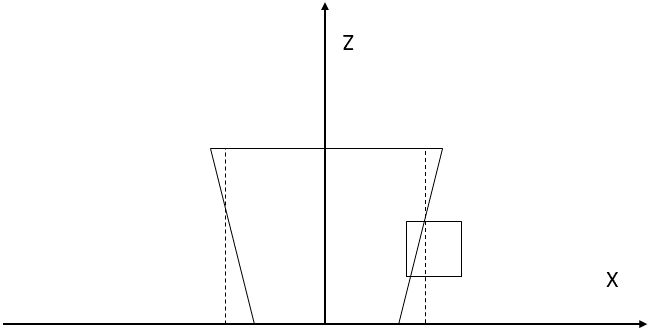
\includegraphics[width=\linewidth]{images/frustumbox.png}
	\caption{Top view of the culling processes. The trapeze represents the portal frustum. The square represent the bounding box of the object. The dotted rectangle can be used instead of the portal frustum for the culling. }
	\label{fig:frustumbox}
\end{figure}

Figure~\ref{fig:frustumbox} shows the portal frustum in camera space as well as the \gls{aabb} of the object. Instead of testing against the frustum, the test is performed against the dotted rectangle, which is also an \gls{aabb}. It is constructed by unprojecting the \gls{psb}['s] x- and y-components using the object's \gls{aabb}'s far z-component, as this is the point where the frustum is the biggest, while still being in the object's \gls{aabb}'s z-range. Only x- and y-components need to be tested against this box, as the z-component was tested already.


The instance count of the object when rendered should correspond to the number of times the test succeeded. However, the gl\_InstanceIndex cannot be used directly anymore to find the correct view matrix and stencil value. Additional information must be passed to the vertex shader. For example, an array of stencil values/view matrix accessed via gl\_InstanceIndex.

\section{Draw Indirect}
Instead of using \textit{drawIndexed}, an implementation could use \textit{drawIndexedIndirect}. This way only a single draw command is needed to render all objects multiple times. Additionally, a portal's fragment shaders could manipulate the values in the draw indirect buffer. If less portals than the maximum visible \gls{portalcount} is visible, there can be fewer instances. Similar to the approach of section~\ref{section:cullingportals} the downside is that \textit{gl\_InstanceIndex} cannot be used directly anymore in the shaders, and the real value must be obtained via buffer writes and reads. But when implemented correctly, no unneeded instances are drawn. The current implementation produces degenerate triangle instead of skipping the whole instance. It needs to be measured whether this approach improves performance. Additionally, adjusting instance counts could be difficult or not yield much benefit when this approach is combined with the approaches of section~\ref{section:cullingportals} and section~\ref{section:portalfrustumculling}.

\section{Reduce Depth Attachment Count}

In section~\ref{section:dynamicportalinstancerendering} a manual stencil buffer was introduced. This means the depthstencil attachment is now exclusively used for the \gls{fardepthbuffer}. When rendering portals, the depth values are written into the \gls{writenearbuffer}, as well as the \gls{fardepthbuffer}, which is used for the depth test. At the end of each recursion, the \gls{fardepthbuffer}'s contents are no longer needed, and it must be cleared. The values in the \gls{fardepthbuffer} and the  \gls{writenearbuffer} are almost the same. The only difference is that the \gls{fardepthbuffer} contains the depth values from rendering the objects. However, for later subpasses there is no real difference, as the manual stencil test discards fragments that would read at locations, where no portal was drawn. This means that the \gls{fardepthbuffer} can be used as the next \gls{readnearbuffer}. The \gls{writenearbuffer} is not needed anymore. However, other means must then be found to detect portal front and back faces, as described in section~\ref{section:portalzfighting}.

\chapter{Visual Improvements}
Performance is not the only area where the prototype can be improved. Currently the prototype lacks proper support for lights, shadows and transparent objects. This section will cover how these could be implemented and what difficulties arise in the presence of transformative portals.

\section{Shadows and Lighting}
Due to time reasons, the prototype has no shadows and only one directional light was implemented. This section covers an approach that would have been used, if time had allowed. If no care is taken, visual seams can appear at portal locations. For instance, shadows could appear cut of or appear out of nowhere in the presence of a portal.

\subsection{Portal Shadow Mapping}
One approach would be a modified version of shadow mapping. In the presence of transformative portals an occluder is not enough for an object to be considered in the shadow. Light might travel through a portal and light it indirectly.

The rendering of shadows maps uses the same approach as rendering the regular scene with multiple portal recursions. The scene is rendered from the light source's view and the depth values are stored in the shadow map. However, in addition to the depth values, the shadow map must also store the view matrix used for rendering the fragment. This should be in form of an index to save space.

When rendering the scene, the shadow test is performed. However, as it is not known whether the light travelled through a portal or lit the fragment directly. It is possible that the same fragment can be lit by the same light multiple times, using different portals. They need to be regarded as separate dynamic lights which share their shadow map. 

For each portal permutation the light could have travelled through, the corresponding teleport matrices must be applied to the light position. Then the position on the shadow map is calculated using that transformed light's position. The shadow map's matrix is compared against the matrix used to transform the light position. If they match the light could illuminated the fragment by travelling through this portal combination. The regular depth test can to be is performed using the transformed light position. If the matrices do not match the object is not lighted by this light-portal permutation but can still be lit by latter combinations.


\subsection{Lighting}
For lighting, only a directional light was implemented. With directional light it is the least noticeable when it is not handled correctly. Especially when portals are placed that the direction light is almost parallel to them.
Lighting is also difficult as it is possible that a fragment can be lit by the same light multiple times. For shadow casting lights, information from the shadow map can be used to detect from where a fragment is lit. If the object does not lie in the shadow for a portal-light combination, the lights position used for accessing the shadow map can be used for lighting calculations.

However, for lights without shadow maps, lighting seems impossible. Lighting a fragment for possible portals the light could have travelled through would create incorrect results and is computationally expensive. 


\subsection{Portals as Light Source}
\label{section:portalsaslights}
Performing doing correct lighting and shadows is expensive. Depending on the use case a potential solution would be to perform lighting and shadowing as though portals did not exist. To hide the seams at portal locations, the portals could behave as a very bright point light. Fragments would appear almost fully lit and shadows would fade out near portals. All fragments close to the portals would be lit the same and not seams would be visible.

However, this has the downside that the location of portals is very visible. If this is not desired the scene must be designed in a way that there are always lights near portals or only use one directional light without shadows and no other light sources.


\section{Transparent Objects}
Transparent objects are not supported in the prototype, but there is nothing that would stop implementing them. They would be rendered very similar to regular approaches: First, everything opaque is rendered, including all portal recursions. After that, the transparent objects are drawn back to front, starting from the last recursion and ending with the initial recursion \cite{lecture:portalProblems}.

However, the far and near depth as well as stencil information of all recursions must be available. This could be done by saving each buffer, instead of reusing and clearing them. Another approach to restore the stencil and \gls{fardepthbuffer} for the previous recursion. This would work similar to SEAM sealing of \textcite{schmalstieg:1999:sewing}. The latter approach would need less textures but more computations.

\chapter{Portal Capability Improvements}
While the portal in the prototype are already functional, they are lacking in a few areas. Improving the capabilities of portals broadens the spectrum of portal applications. The following sections discuss possible portal capability improvements.


\section{Portal Physics}
\label{section:portalphysics}
The implementation currently only supports collision for the camera. Depending on the use case for portals, portal physics are needed. There are several problems that must be solved to allow for realistic portal physics.

\subsection{Portal Edges}
Portals that are not completely placed on solid objects either must have collision on their edges or allow slicing objects into pieces.

\begin{figure}[h]
	\centering
	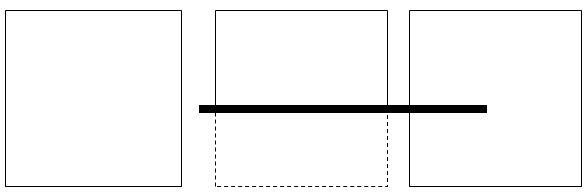
\includegraphics[width=\linewidth]{images/edgecollision.png}
	\caption{A box represent an object, while the thick line represents a planar portal. It is not clear what should happen to the right object}
	\label{fig:edgecollision}
\end{figure}

Figure~\ref{fig:edgecollision} illustrates the possible problem: The left object passes the portal, the middle object goes through the portal, with the dotted part being present at another location. However, it is not clear what should happen to the right object. This case could be prevented via collision on the portal edge. Another solution is to slice the box on the portal's edge so that one part travels through the portal, while the other passes it. Watertight portals do not have edges, so this problem cannot occur for them.

\subsection{Halfway through Objects}
For an object with a volume it is possible that only a part of it travelled through the portal (see figure~\ref{fig:edgecollision}). The two parts of the object must exist in two different locations. However, duplicating the object is not enough. It must also be insured that an object piercing a portal from the front, cannot be seen or interacted with from the back. Additionally, the physics state must the same for both parts. Special care must be taken for the player's avatar. If the player is halfway through the portal, they should not see part of their avatar directly at their viewing location. Some of these problems can be seen in the lecture of \textcite{lecture:portalProblems}.


\section{Non-Translating Portals}
The implemented portals have two endpoints. Objects move through one endpoint, appear at the other. However, it is also possible that the portals don't move the object. In this case there is just one portal.

Entering the portal would apply an operation (e.g. multiplying by matrix), leaving it applies the inverse operation. Instead of rendering two endpoints, only one portal is rendered. Back and Front face detection needs to be used to decide which operation to apply.

This works only for operations which do not move the position of an object. One exception would be a rotation. However, the portal shape must look the same after applying the rotation to it. E.g. a sphere could allow for any rotation. A cube only for rotation in intervals of 90 degrees. Inverting or the scale of an object would another case.



\subsection{Arbitrary Operations}

In the prototype the portals only apply transformative operations in using matrices. Non-translating portals could also allow completely arbitrary operations.

A portal's operation could change render parameters. These parameters can be stored similar to storing the view matrices. One example, inspired by \textcite{borst:2009:real}, would to mark pixels when one parameter has a specific value. Later in a post process the marked pixels could be modified, e.g. with image warping effects. Another example, inspired by magic lenses would be a parameter to conditionally render objects. This would allow the creation of parallel world, which can share some of their objects.

Inspired by the works of \textcite{ryall:2005:temporal} as well as \textcite{tiesel:2009:composable}, another very interesting form of a non-translating portal would be a temporal portal. Instead of moving objects through space it moves them through time. However, even more care than described in section~\ref{section:portalphysics} must be taken, such as objects colliding with its past self, changing the presence by changing the past etc.


%\section{Form changing portals ?}
%{multiple portals, represented by one mesh}
%{portals as mathematical function, implicit surfaces }

%\section{Change portal connections ?}



\section{World Wrapping}
World wrapping enables infinite worlds, which repeat themselves. When an object moves outside one end of the wrapped world it is teleported to the opposite end. It is possible to implement world wrapping using the prototype's transformative portals. However, portals used for world wrapping have special properties: They can be represented by infinite planes and the scene exists only inside those planes. No object is outside these planes. This means the problem described by figure~\ref{fig:bananajuce} cannot occur.

This allows for special optimizations: The stencil test is not needed, as the only repeated scene will be drawn at that location. The near buffer is also not needed, as the multiple scenes cannot overlap each other. This means drawing the actual portals is not necessary. All world instance can be drawn at once, using instanced drawing, with each world instance using the corresponding view matrix.

However, if portals are already present it is probably better to just define big portal planes. Otherwise, the process that was just described needs to be used also for each world that is drawn for a portal.


\chapter{Conclusion}

%\section{Implementation summary}

Previous works use a depth-first approach to render transformative portals. This thesis presents another approach using breadth-first. Additionally, it supports arbitrary portals defined by triangle meshes. While arbitrary portals are becoming more common, they are not supported everywhere.

On the authors machine, the prototype performed quite well. Scenes with ten or more portals ran smoothly. However, in most settings the \gls{recursioncount} cannot be higher than four. Higher recursion counts took increasingly much longer to render exceeding the maximum time available for real time applications.



The implementation used many techniques found in previous works to render transformative portals. However, two key improvements were implemented, which the author has not yet seen in other works.

The first is the visible portal count algorithm. It to performs an operation during the fragment shader which is similar to an occlusion query. This allowed for a higher number of portals in a scene, as long as only a limited number of them were visible. While this could be used in depth-first portal rendering, the author has not yet seen something similar implemented.

The second is the use of instanced drawing, which is probably one of the biggest benefits of breadth-first portal rendering. While instanced drawing is commonly seen, the author has not yet seen its use in the context of transformative portals. Instanced drawing helped to improve performance by drastically reducing the number of operations sent to the \gls{gpu}, which improved the overall performance significantly. No thorough measurements for comparison were made, but after adding instanced drawing, the time to render was only a sixth of the time before. 

Furthermore, the prototype was created using only a single render pass, with multiple subpasses. This potentially allows the \gls{gpu} to optimize. The number of subpasses needed scales linearly to the \gls{recursioncount}. However, this thesis only proved that breadth-first is a viable approach, which allows for improvement opportunities exclusive to it. No measurements were performed to test whether depth- or breadth-first performs better in different situations.

One downside of instanced drawing is that the regular stencil test cannot be used. As the reference value cannot be changed between instances, stencil testing and discarding fragments was performed in the fragment shader. This prohibited using early fragment tests. This was not seen as much of a downside, as the dual depth buffer also required also required manual testing and discarding, prohibiting early fragment tests anyway. However, for applications that do not need to use a dual depth buffer, this can be considered a downside. Furthermore, the use of manual test requires inserting them in every shader, which is inconvenient.

Another problem is that the prototype still has a limit for the maximum  number portals in a scene. This is because the \glspl{viewmatrix} are calculated for every portal combination, even if that \gls{viewmatrix} is needed for rendering. However, this problem should be relatively easy to fix in future. Many optimisations discussed in section~\ref{section:performanceimprovements} could either speed up the calculation or reduce the needed matrix count considerably.

An interesting discovery were portals which are defined by watertight meshes. They are not very useful as static portals, but when modified dynamically they could allow for effects such as swapping or rotating subspaces. Additionally, the holes of almost watertight portals behave and look like a portal for the user, while the actual portal seems not to be present. But in reality, the opposite is true.


\section{Possible Improvements}

While the current version of the prototype already has some use cases, there are still many possibilities for improvement. However, not every improvement opportunity is useful for every application. Three directions were identified.

In the visual area, the prototype can be improved by supporting more than a single directional light for shading as well as adding shadows. Depending on the application these may be implemented in a less exact way to improve performance. The resulting artefacts can be hidden with well placed light sources. Additionally, support for transparent objects can be added.

The portal's capabilities can be improved. Non-translating portals, portals with more than just transform changes and physical portals are not included in the prototype. Such improvements increase the range of use cases for portals in games or similar applications.

Lastly, the performance can be improved. Not all performance opportunities are equal. The most performance is likely to be gained by using culling techniques. Performing visibility culling on portals (see section~\ref{section:cullingportals}) seems to be the most important one its calculations can be reused for the other culling techniques. Another important opportunity is to improve the calculation of the view matrices by removing the need for matrix inversion. This seems to provide some gain for almost no work and is strongly recommended.

The introduction of visibility culling might have strong impact on the prototype and some choices need to be revisited. Unless extra steps are taken to prevent false visible portals (see section~\ref{section:falsevisible}) the dynamic calculation of visible portals would become almost obsolete. In such a case the extra work introduced via indirections and synchronisation might not be worthwhile.

Additionally, there are some possibilities that would require changes in the graphics \gls{api}.

At the moment it is not possible to allow early fragment testing, as manual checks against the near buffer need to be performed in the shader. However, if in the future the depth test allows the use of a near buffer, some decisions there are some improvement opportunities. It might be worthwhile to remove instanced drawing, in favour of early fragment tests. If stencil export for shaders prior to rasterization are available, instancing could still be used.

Another opportunity would be a separation of the comparison and write operations of a depth test and stencil test. If the writes only happen after a fragment shader is executed without calling discard, the comparison operation could happen early.

\section{Possible Applications}
One area where the findings of this thesis can be applied are video games. Portals may not only serve a gameplay mechanic, but can be used for other purposes as well, such as seamless transitions between scenes similar to the work of \textcite{schmalstieg:1999:sewing}. In general video games only use sparingly number of portals. The breadth-first approach might offer better performance, allowing for higher \glspl{portalcount}. As previously stated, it needs to be tested whether this approach actually improves performance.

Mirrors are portal variants that are much more common than transformative portals. The techniques described in this thesis can be applied to them as well. In addition, mirrors are often plane shaped. The near buffer could be replaced by user defined clip planes.


%\subsection{Improving Portal based occlusion culling}
The technique that calculates the number of previous visible portals could be adapted and used together with portal-based occlusion culling. Objects within cells are rendered using draw indirect. This allows changing the instance count of the objects and can effectively disable them. All objects within are cell are only enabled, if at least a fragment of the corresponding portal is drawn. This can be achieved by initially setting the instance count to 0 for all object. Then in a portal's fragment shader the instance count can be set to 1, which only happens if at least one fragment is drawn. With Vulkan extension such as VK\_EXT\_conditional\_rendering and VK\_NV\_representative\_fragment\_test this approach can be improved even further \cite{khronos:vulkan:spec1.1}

%Depending on available \gls{gpu} extension this approach can be further improved. When using Vulkan the extension VK\_EXT\_conditional\_rendering can be used. This removes the need for an draw indirect buffer and looping over all its elements and setting the instance count individually \cite{khronos:vulkan:spec1.1}.

%Another useful extension for this purpose are representative fragment tests. If any primitive produces one or more fragments that all pass the fragment test one or more of those fragments are chosen. All other fragments are discarded. As its only important to detect whether or not at least one fragment is visible, this can reduce the number of unnecessary fragments. The test can be enabled with GL\_NV\_representative\_fragment\_test and VK\_NV\_representative\_fragment\_test for OpenGL \cite{khronos:openGL:representative} and Vulkan\cite{khronos:vulkan:spec1.1} respectively.


%\section*{Image based portal rendering - likely does not work well}
%For each portal render its view into texture, if the view contains another portal, save the id and uv coordinates. Make a copy of the textures. Then process textures again, overwriting previously marked portals. This is done by fetching the pixel with the saved uv coords from that texture. This pixel may be a colour or could be a portal mark. Repeat this process until there are no more portal markings or when threshold is exceeded.
%Bad scaling with maxiumum portal count
%Good scaling with recursions: as drawing a portal's contents also draws its recursion contents, doubling the number of recursions with each step -> 1,2,4,8,16...
%Might look ugly, wrong perspective


%For debugging OpenGL offers debug output to obtain details about errors, performance warnings and other useful information. They can be obtained via a debug message callback or by querying them from a message log \cite{khronos:openGL:spec4.6}. In Vulkan validations layers are used for finding errors. In Vulkan \gls{api} calls can be intercepted by layers. They perform whatever operation defined by their implementation before maybe passing them to the actual function. Validation layers are layers w

%They validate the parameters, before passing them to the actual function. How errors are reported depends on the prototype of the layer.. Multiple layers can be active and are called each one sequentially before calling the actual function. \cite{khronos:vulkan:spec1.1}












